% documentclass options:
% ngerman is needed for hyphenation if the thesis contains parts written in German
% BCOR is binding correction
% if you'd rather have a one sided thesis, add `oneside' to the documentclass
\documentclass[11pt, a4paper, BCOR=10mm, english, ngerman, oneside]{scrbook}
% include all packages and define commands in setup.tex

%------------------------------------------------------------------------------
%       package includes
%------------------------------------------------------------------------------
    % font encoding is set up for pdflatex, for other environments see
    % http://tex.stackexchange.com/questions/44694/fontenc-vs-inputenc
    \usepackage[T1]{fontenc}  % 8-bit fonts, improves handling of hyphenations
    \usepackage[utf8x]{inputenc}
    % provides `old' commands for table of contents. Eases the ability to switch
    % between book and scrbook
    \usepackage{scrhack}


    % ------------------- layout, default -------------------
    % adjust the style of float's captions, separated from text to improve readabilty
    \usepackage[labelfont=bf, labelsep=colon, format=hang, textfont=singlespacing]{caption}
    \usepackage{chngcntr}  % continuous numbering of figures/tables over chapters
    \counterwithout{equation}{chapter}
    \counterwithout{figure}{chapter}
    \counterwithout{table}{chapter}

    % Uncomment the following line if you switch from scrbook to book
    % and comment the setkomafont line
    %\usepackage{titlesec}  % remove "Chapter" from the chapter title
    %\titleformat{\chapter}[hang]{\bfseries\huge}{\thechapter}{2pc}{\huge}
    \setkomafont{chapter}{\normalfont\bfseries\huge}

    \usepackage{setspace}  % Line spacing
    \onehalfspacing
    % \doublespacing  % uncomment for double spacing, e.g. for annotations in correction

    % ------------------- functional, default-------------------
    \usepackage[dvipsnames]{xcolor}  % more colors
    \usepackage{array}  % custom format per column in table - needed on the title page
    \usepackage{graphicx}  % include graphics
    \usepackage{subfig}  % divide figure, e.g. 1(a), 1(b)...
    \usepackage{amsmath}  % |
    \usepackage{amsthm}   % | math, bmatrix etc
    \usepackage{amsfonts} % |
    \usepackage{calc}  % calculate within LaTeX
    \usepackage[unicode=true,bookmarks=true,bookmarksnumbered=true,
                bookmarksopen=true,bookmarksopenlevel=1,breaklinks=false,
                pdfborder={0 0 0},backref=false,colorlinks=false]{hyperref}


    %==========================================
    % You might not need the following packages, I only included them as they
    % are needed for the example floats
    % ------------------- functional, custom -------------------
    \usepackage{algorithm,algpseudocode}
    \usepackage{bm}  % bold greek variables (boldmath)
    \usepackage{tikz}
    \usetikzlibrary{positioning}  % use: above left of, etc

    % Improves general appearance of the text
    \usepackage[protrusion=true,expansion=true, kerning]{microtype}

%------------------------------------------------------------------------------
%       (re)new commands / settings
%------------------------------------------------------------------------------
    % ----------------- referencing ----------------
    \newcommand{\secref}[1]{Section~\ref{#1}}
    \newcommand{\chapref}[1]{Chapter~\ref{#1}}
    \renewcommand{\eqref}[1]{Equation~(\ref{#1})}
    \newcommand{\figref}[1]{Figure~\ref{#1}}
    \newcommand{\tabref}[1]{Table~\ref{#1}}

    % ------------------- colors -------------------
    \definecolor{darkgreen}{rgb}{0.0, 0.5, 0.0}
    % Colors of the Albert Ludwigs University as in
    % https://www.zuv.uni-freiburg.de/service/cd/cd-manual/farbwelt
    \definecolor{UniBlue}{RGB}{0, 74, 153}
    \definecolor{UniRed}{RGB}{193, 0, 42}
    \definecolor{UniGrey}{RGB}{154, 155, 156}


    % ------------------- layout -------------------
    % prevents floating objects from being placed ahead of their section
    \let\mySection\section\renewcommand{\section}{\suppressfloats[t]\mySection}
    \let\mySubSection\subsection\renewcommand{\subsection}{\suppressfloats[t]\mySubSection}


    % ------------------- marker commands -------------------
    % ToDo command
    \newcommand{\todo}[1]{\textbf{\textcolor{red}{(TODO: #1)}}}
    \newcommand{\extend}[1]{\textbf{\textcolor{darkgreen}{(EXTEND: #1)}}}
    % Lighter color to note down quick drafts
    \newcommand{\draft}[1]{\textbf{\textcolor{NavyBlue}{(DRAFT: #1)}}}


    % ------------------- math formatting commands -------------------
    % define vectors to be bold instead of using an arrow
    \renewcommand{\vec}[1]{\mathbf{#1}}
    \newcommand{\mat}[1]{\mathbf{#1}}
    % tag equation with name
    \newcommand{\eqname}[1]{\tag*{#1}}


    % ------------------- pdf settings -------------------
    % ADAPT THIS
    \hypersetup{pdftitle={The great title!},
                pdfauthor={FirstName LastName},
                pdfsubject={Undergraduate thesis at the Albert Ludwig University of Freiburg},
                pdfkeywords={deep learning, awesome algorithm,  undergraduate thesis},
                pdfpagelayout=OneColumn, pdfnewwindow=true, pdfstartview=XYZ, plainpages=false}


    %==========================================
    % You might not need the following commands, I only included them as they
    % are needed for the example floats

    % ------------------- Tikz styles -------------------
    \tikzset{>=latex}  % arrow style


    % ------------------- algorithm ---------------------
    % Command to align comments in algorithm
    \newcommand{\alignedComment}[1]{\Comment{\parbox[t]{.35\linewidth}{#1}}}
    % define a foreach command in algorithms
    \algnewcommand\algorithmicforeach{\textbf{foreach}}
    \algdef{S}[FOR]{ForEach}[1]{\algorithmicforeach\ #1\ \algorithmicdo}


\begin{document}
    \pagestyle{empty} % no header and no page number
    % disable hyper links to remove warning "destination with same identifier"
    % this means within this section nothing can be referenced with a hyperlink
    \hypersetup{pageanchor=false}
    
    % enable/disable, depending on your chosen language
    \begin{titlepage}
\begin{center}

\newcommand{\HorizontalLine}{\rule{\linewidth}{0.3mm}}

{\Large Master Thesis}\\[2cm]


% 
\begin{spacing}{3}
    {\huge \bfseries Recommender System for } \\
    {\huge \bfseries Galaxy Tools and Workflows } \\
    {\Large \bfseries (Find similar tools and predict next tools in workflows) }\\[2cm]
\end{spacing}


{\Large Anup Kumar } \\[2cm]


\begin{tabular}[hc]{>{\Large}l >{\Large}l}
  Advisor: & Dr. Björn Grüning \\[0.3cm]
  Examiners: & Prof. Dr. Rolf Backofen, Prof. Dr. Wolfgang Hess \\[1.2cm]
\end{tabular}
\vfill  % move the following text to the bottom

\Large {
    University of Freiburg\\
    Faculty of Engineering\\
    Department of Computer Science\\
    Chair for Bioinformatics\\[1cm]
    July, 2018
    \\
}
\end{center}
\end{titlepage}

% title page back
\ \vfill \ \\  % at least one space required before vfill
\
\textbf{Writing period}            \smallskip{} \\
09.\,01.\,2018 -- 09.\,07.\,2018   \bigskip{} \\
\
\textbf{Examiners}                 \smallskip{} \\
Prof. Dr. Rolf Backofen and Prof. Dr. Wolfgang Hess               \bigskip{} \\
\
\textbf{Advisor}                   \smallskip{} \\
Dr. Björn Grüning

    
    \pagestyle{plain} % remove chapter name from top, page number at the bottom
    \frontmatter  % roman page numbers
    % official declaration from the examination office; to be sure double
% check the wording on their website
% (https://www.tf.uni-freiburg.de/studies/exams/thesis/thesis_formatting.html#erklaerung)

\chapter*{Declaration}

I hereby declare, that I am the sole author and composer of my thesis and that no other sources or learning aids, other than those listed, have been used. Furthermore, I declare that I have acknowledged the work of others by providing detailed references of said work.  \newline
I hereby also declare, that my Thesis has not been prepared for another examination
or assignment, either wholly or excerpts thereof.
\\[3\normalbaselineskip]
\begin{tabular}{p{\textwidth/2} l}
  \rule{\textwidth/3}{0.4pt}   &   \rule{\textwidth/3}{0.4pt} \\
  Place, Date                  &   Signature
\end{tabular}

    \chapter*{Acknowledgment}
Acknowledgement
    \chapter*{Abstract}
The study explores two concepts to devise a recommendation system for Galaxy. A recommendation system can apprise a Galaxy user of the latent relations that exist among the tools in terms of their functions and types. Exhibiting an array of next possible tools at each step of picking a tool while creating workflows can also be a meaningful addition to this system. 

To find similarities among tools, we need to extract information about each tool from its attributes like name, description, input and output file types and help text. We take into account these attributes one by one and compute similarity matrices. We compute three similarity matrices, one each for input and output file, name and description and help text attributes. Each row in a similarity matrix holds similarity scores of one tool against all the other tools. These similarity scores depend on the similarity measures (jaccard index and cosine similarity) used to compute the score between a pair of tools. To combine these matrices, one simple solution is to compute an average. But, assigning equal importance weight to each matrix might be sub-optimal. To find an optimal combination, we use optimization to learn importance weights for the corresponding rows for each tool in the similarity matrices. To define a loss function for optimization, we use a true similarity value based on the similarity measures. The similarity scores are positive real numbers between $0$ and $1$. We take an array of $1.0$ as the true value.

Next task analyzes workflows to predict a set of next tools at each stage of creating workflows. While creating workflows, it would be convenient to leaf through a set of next possible tools as a guide. It can assist the less experienced (Galaxy) users in creating workflows when they are unsure about which tools can further be connected. In addition, it can curtail the time taken in creating a workflow. To achieve that, we need to learn the connections among tools in order to be able to predict the next possible ones based on the previously connected tools. To preprocess the workflows to make them usable by downstream machine learning algorithms, we compute all the paths bridging the starting and end tools in all workflows. We follow a classification approach to predict the next tools and use LSTM (long short-term memory), a variant of recurrent neural networks. It performs well for learning long range, sequential and time-dependent data (tools connections) \cite{LiptonKEW15, SakSB14}. We report the accuracy as precision.


\chapter*{Zusammenfassung}

    \tableofcontents
    %\listoffigures
    %\listoftables
    %\listofalgorithms
    \hypersetup{pageanchor=true}  % re-enable hyperlinking

    \mainmatter  % Arabic page numbers
    \chapter{Introduction}\label{chap:introduction}
\section{Galaxy}
Galaxy{\footnote{\url{https://usegalaxy.eu/}}} is an open-source biological data processing and research platform. It supports numerous types of extensively used biological data formats like FASTA, FASTAQ, GFF, PDB and many more. To process these datasets, it offers tools and workflows which transform these datasets (figure 1). Each tool and workflow furnish exclusive means to process datasets. A simple example of this processing is to merge two compatible datasets to make one. Another example can be to reverse complement a sequence of 
nucleotides\footnote{\url{https://usegalaxy.eu/?tool_id=MAF_Reverse_Complement_1&version=1.0.1&__identifer=zmk9dx9ivbk}}.

\begin{figure}[h]
\begin{centering}
    {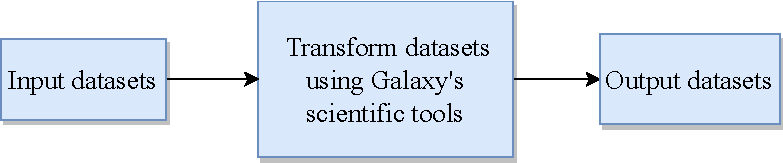
\includegraphics[scale=0.8]{figures/image_Galaxy_1.pdf}}
    \caption[Basic flow of dataset transformation]{\textbf{Dataset transformation}: The images shows a general flow of dataset transformation using Galaxy tools and workflows.}
\end{centering}
\end{figure}

A tool is a data-transforming entity. The tools are classified into multiple categories based on their functions and types. For example, the tools which manipulate text like replacing texts and selecting first lines of a dataset are grouped together under "Text Manipulation" category. These tools form the building blocks of workflows. The workflows are data processing pipelines where a set of tools are joined one after another and protrude from a tool to make branches. The connected tools should to be compatible with each other. It means that the output file types of one tool should be present in the input file types of the next tool.

\section{Galaxy tools}
A tool entails a specific function. It consumes a dataset, brings about some transformation and produces an output dataset which can be fed to other tools. It has multiple attributes which include its input and output file types, name, description, help text and so on. These attributes carry more information about a tool. When we look at the collective information about all these attributes for a set of tools, we recognize that some of them have comparable functionalities. There are tools which share affinities in their respective functions and the input and output file types they are glued to. For example, a tool "hicexplorer hicpca" \footnote{\url{https://usegalaxy.eu/?tool_id=toolshed.g2.bx.psu.edu/repos/bgruening/hicexplorer_hicpca/hicexplorer_hicpca/2.1.0&version=2.1.0&__identifer=5kcqmvb71gx}} has an output type named "bigwig". If there is a tool which also has "bigwig" as its input and/or output type, we consider there can be some similarity between these tools as they do transformations on similar types of files. In addition, we can find similar functions of tools by analyzing their "name" and "description" attributes. Let's take an example of two tools (figure 2):
 
\begin{figure}[h]
\begin{centering}
    {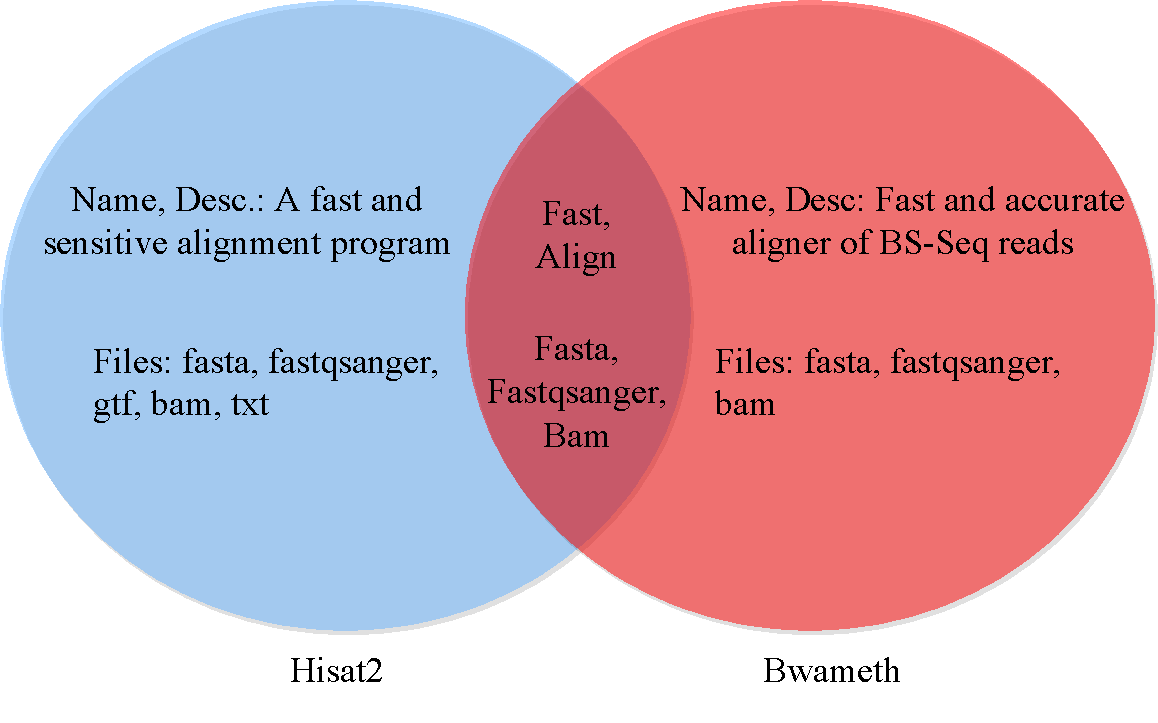
\includegraphics[scale=0.5]{figures/Venn_common_tools_info.pdf}}
    \caption[Common features of two tools using venn diagram]{\textbf{Common features of two tools using venn diagram}: The venn diagram shows the common features for two tools - linear regression and logistic regression. Based on these common features, we assess the extent of similarity between them.}
\end{centering}
\end{figure}

In figure 2, we take two tools - "linear regression" and "logistic regression" and collect their respective information from their input and output file types, name and description attributes. We can see that these tools share some features. They share a similar function of doing regression and few file types are also common. Similarly, if we extrapolate this notion of finding similar features among all the tools, we hope to find a set of similar tools for each tool. Also, it is possible that we end up with an empty set of similar tools for a tool.

\section{Motivation}
From figure 2, we see that there can be tools which share characteristics. Galaxy has thousands of tools having a diverse set of functions. Moreover, new tools keep getting added to the older set of tools. From a user's perspective, it is hard to keep knowledge about so many tools. It is important to make a user aware of the presence of new tools added. If there is a model which dispenses a clue that there is a set of say $n$ tools which are similar to a tool, it would give more options to a user for her/his data processing. 

\begin{figure}[h]
\begin{centering}
    {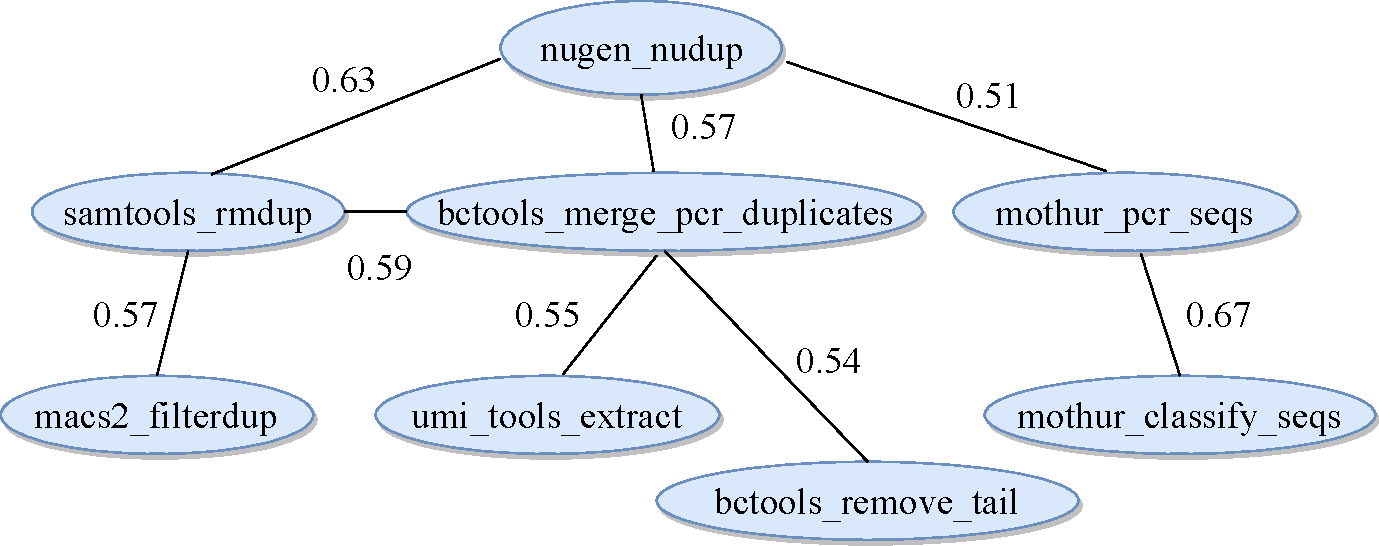
\includegraphics[scale=0.6]{figures/tools_sim_know_graph.pdf}}
    \caption[Similarity knowledge graph]{\textbf{Similarity knowledge graph}: The graph defines a network of relationship among the tools using the similarity scores between a pair of nodes (tools). The real numbers on an edge is the relation strength between two nodes.}
\end{centering}
\end{figure}

To elaborate it more, let's take an example of a tool "nugen nudup" \footnote{\url{ https://toolshed.g2.bx.psu.edu/repository?repository_id=4f614394b93677e3 }}. It is used to find and remove PCR duplicates. The similar tools for it can be "samtools rmdup" and "bctools merge pcr duplicates" which work on related concepts. These similar tools would further have their respective set of similar tools thereby making a network of related entities (tools). This "knowledge network" can help a user find multiple ways to process her/his data and exhibits "connectedness" among tools. The strength of this relation may vary from being small to large. To ascertain that, this study learns a continuous representation of the relation strength. Figure 2 shows how this knowledge graph can evolve. First, we find similar tools for "nugen nudup" and connect them to their source tool specifying the similarity values as real numbers at the edges. These similar tools further have their own sets of similar tools and so on.


    \chapter{Approach}\label{chap:approach}
In this section, we provide a layout of our approach to find similar tools. It includes procedures to extract and clean tools data, learn vectors for each tool, find similarity (correlation) matrices and optimize the combination of these matrices to estimate a final similarity matrix (figure 4). 
\section{Extract tools data}    
As Galaxy is an open-source project, the repositories of tools are stored at GitHub\footnote{One example:\url{https://github.com/galaxyproject/tools-iuc/tree/master/tools}}. In these tool repositories, the xml files which start a "tool" tag belong to a tool. We read all of these xml files, extract information from a few of the tool attributes and collect them in a tabular file. This tabular file contains the information about all the tools.

\begin{figure}[h]
\begin{centering}
    {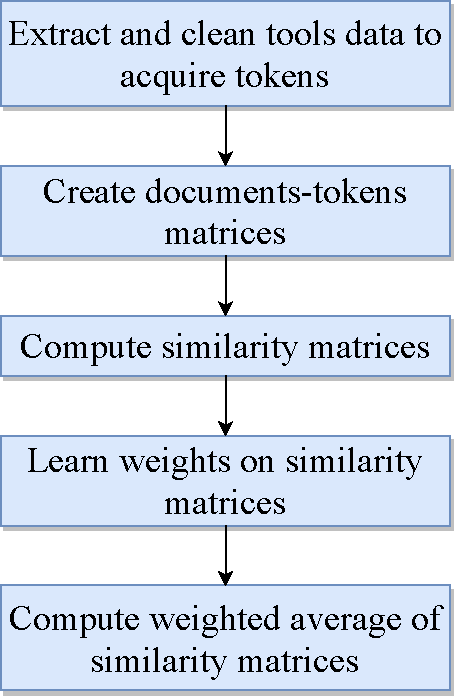
\includegraphics[scale=0.7]{figures/tool_sim_flow.pdf}}
    \caption[Sequence of steps to find similar tools]{\textbf{Sequence of steps to find similar tools}: The flowchart shows a series of steps used to establish similarity among tools using approaches from natural language processing to compute text similarity scores and optimization to combine optimally.}
\end{centering}
\end{figure}
    
\subsection{Select tools attributes}
A tool has multiple attributes like input and output file types, help text, name, description, citations and more. But all of these attributes are not important and do not generally identify a tool exclusively. To collect distinguishing information about a tool, we consider only these attributes:
\begin{itemize}
	\item Input and output file types
	\item Name and description
	\item Help text
\end{itemize}
Moreover, we combine the input and output file types and name and description respectively as they are of similar nature. These combined attributes give complete information about a tool's file types (input and output types) and its functionality (name and description). Further, we take help text attribute as well which is larger in size compared to the previous two. It can also be empty for some tools. Apart from being large in size, it is noisy. It provides more information about the usage of a tool. Generally in the first few lines, it gives a detailed explanation of a tool's functions. Further, it explains how the input data should be supplied to a tool or how an input data looks like. Much of the information contained by this attribute is not important to clearly distinguish a tool. Hence, we decide to use only the first few lines ($4$ lines) of text present in help text attribute of a tool which illustrates its core functionality. The rest of the information in help text is discarded. The decision to select only the first $4$ lines is empirical.

\subsection{Clean tools data}
\subsubsection{Remove duplicates and stopwords}
    The collected data for tools is raw as it contains lots of commonplace and duplicate items which do not add value. These items should be removed to get $tokens$ which are unique and useful. For example, a tool "bamleftalign" has input files as "bam" and "fasta" and output file as "bam". While combining these file types, we discard the repeated ones. In this case, we consider the file types as "bam" and "fasta". The other attributes we deal with are different from the file types. The files types are already in the form of $tokens$. But, in the attributes like name and description and help text, the words come from English and the explanation contains complete or partially complete sentences. Hence, to process this information, we need strategies that are prevalent in natural language processing\footnote{\url{https://www.ncbi.nlm.nih.gov/pmc/articles/PMC3168328/}}. The sentences we write in English contain many words and has different parts. These parts include subject, object, preposition, interjection, verbs, adjectives, adverbs, articles and many others. For our processing, we need only those tokens (words) which categorize a tool uniquely and do away with multiple parts of speech present in the sentences. For example, a tool named $tophat$ has a name and description as "TopHat for Illumina Find splice junctions using RNA-seq data". The words like "for", "using" and "data" do not give much value as they can be present for many other tools. These words are called as "stopwords"\footnote{\url{https://www.ranks.nl/stopwords}} and we selectively discard them. In addition, we remove numbers and convert all the tokens to lower case.
 
\subsubsection{Use stemming}
After removing duplicates and stopwords, our data is clean and contain tokens which uniquely identify corresponding tools. When we frame sentences, we follow grammar which constrains us to use different forms of the same word in varying contexts. For example, a word "regress" can be used in multiple forms as "regresses" or "regression" or "regressed". They share the same root and point towards the same concept. If many tools use this word in varying forms, it is beneficial to converge all the different forms of a word to one basic form. This process is called stemming\footnote{\url{https://nlp.stanford.edu/IR-book/html/htmledition/stemming-and-lemmatization-1.html}}. We use NLTK\footnote{\url{http://www.nltk.org/}} package for stemming. It enables us to reduce the size to tokens while keeping the meaning of these tokens same across all the tools.

\begin{figure}[h]
\begin{centering}
    {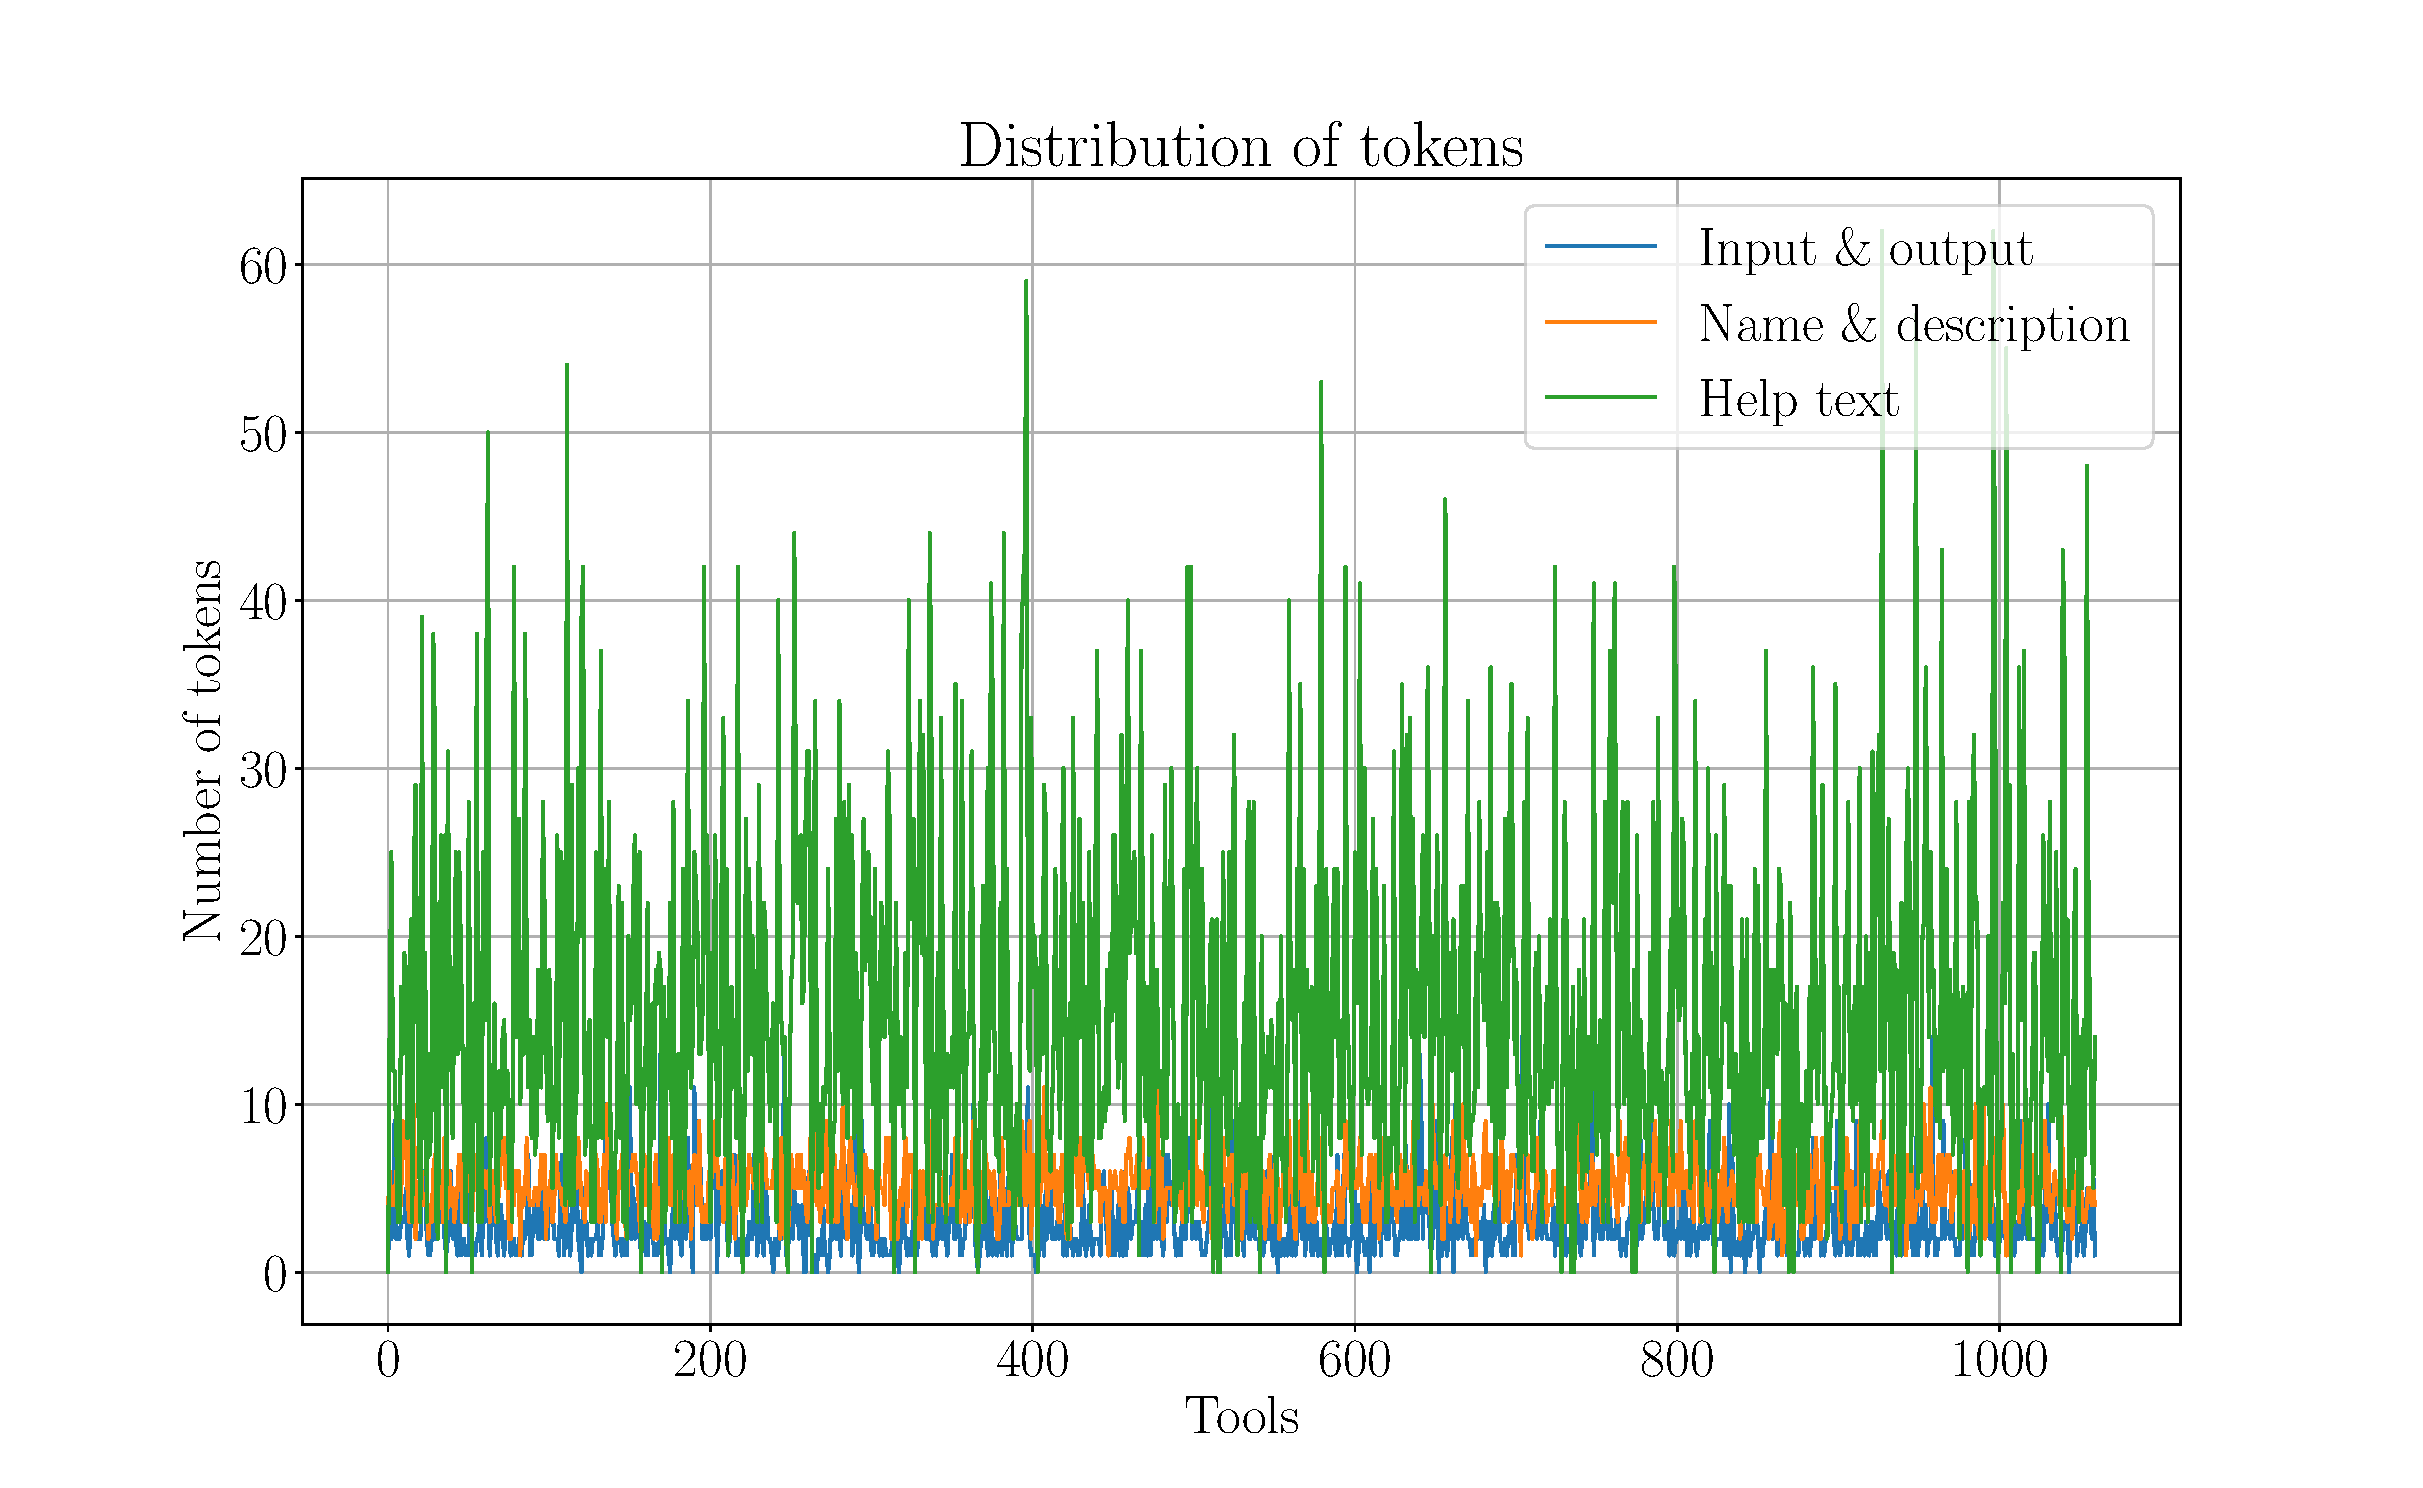
\includegraphics[scale=0.4]{figures/Tokens_dist.pdf}}
    \caption[Distribution of tokens for all the attributes of tools]{\textbf{Distribution of tokens (words) for all the attributes of tools}: The plot shows a distribution of tokens for input and output file types, name and description and help text attributes of tools. The help text attribute contains more number of tokens compared to the other two. The input and output file types attribute contains a lower number of tokens compared to the other two attributes. }
\end{centering}
\end{figure}

\begin{figure}[h]
\begin{centering}
    {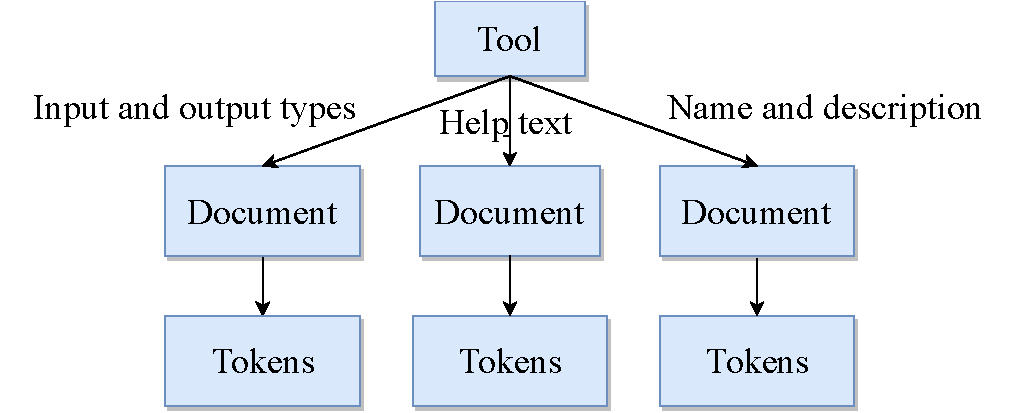
\includegraphics[scale=0.7]{figures/tool-document-tokens.pdf}}
    \caption[Tool, document and tokens]{\textbf{Relationship between a tool, its documents and their tokens}: The image shows that a tool has three documents corresponding to each attribute and each document contains tokens. For all the tools, we have documents equal to the number of tools for each attribute. The number of tokens in each document varies. Minimum number of tokens for any document can be 0.}
\end{centering}
\end{figure}

\subsubsection{Learn relevance for words}
From now on, we use a term "token" for each word. For example, a tool's name contains "regress, perform" as a set of tokens (words). After discarding duplicate tokens, stopwords and using stemmed words, we have a set of meaningful tokens for all the three attributes - input and output file types, name and description and help text. We call these sets as "documents" (figure 6). The tokens present in these documents do not carry equal importance. Some tokens are more relevant to a document and some not so relevant. We need to find out importance factors for all tokens in a document. Using these factors, we can arrange them in big, sparse documents-tokens matrix. In these matrices, each row represents a document and each column belongs to one token. To compute these importance factors, we use BM25 (bestmatch25) \cite{Robertson:2009:PRF:1704809.1704810}. Let's associate some variables to be used in explaining this algorithm.

\begin{itemize}
	\item Token frequency\footnote{\url{https://nlp.stanford.edu/IR-book/pdf/06vect.pdf}} ($tf$)
	\item Inverted document frequency ($idf$)
	\item Average document length ($|D|_{avg}$)
	\item Number of documents ($N$)
	\item Size of a document ($|D|$)
\end{itemize}
    
Token frequency ($tf$) specifies the count of a token's occurrence in a document. If a token "regress" appears twice in a document, its $tf$ is $2$. This can also be understood as a weight given to this term. Inverted document frequency for a token is defined as:

\begin{equation}
idf = \log \frac{N}{df}
\end{equation}
 
where $df$ is the count of the documents in which this token is present and $N$ is the total number of documents. If we randomly sample a document, then the probability of this token to be present in this document is $ p_i = \frac{df}{N} $. From information theory, we can say that the information contained by this event is $ - \log p_i $. The entity $idf$ is higher when a token appears in a lesser number of documents. It means that this token is a good candidate for representing that document and thereby, possesses a higher power to distinguish between documents. The tokens which appear in many documents are not good representatives as they tend to be commonplace. Average document length ($|D|_{avg}$) is the average number tokens for all the documents. Size of a document ($|D|$) is the count of all the tokens for that document. 

\begin{equation}
\alpha = (1-b) + \frac{b \cdot |D|}{|D|_{avg}}
\end{equation}

\begin{equation}
tf^* = tf \cdot \frac{k+1}{k \cdot \alpha + tf}
\end{equation}

\begin{equation}
BM25_{score} =tf^* \cdot idf
\end{equation}

where $k$ and $b$ are hyperparameters. Using the equation $4$, we compute the relevance score for each token in all the documents. Table 1 shows scores for a few documents where the tokens are present with their respective BM25 scores. In this way, we arrange document-tokens matrix for all the attributes of tools. For input and output file types, these matrix entries will have only two value, $1$ if a token is present for a document and $0$ if not. For other attributes, relevance scores are positive real numbers. This method of representing documents with their tokens is called vector space model as each document represents a vector of tokens.

\begin{table}[ht]
\begin{center}
    \begin{tabular}{|l|l|l|l|l|l|}
        \hline
        Documents/tokens   & regress & linear & gap & mapper & perform \\ \hline
        LinearRegression   & 5.22 & 4.1 & 0.0 & 0.0  & 3.84 \\ \hline
        LogisticRegression & 3.54 & 0.0 & 0.0 & 0.0  & 2.61 \\ \hline
        Tophat2            & 0.0  & 0.0 & 1.2 & 1.47 & 0.0 \\ \hline
        Hisat              & 0.0  & 0.0 & 0.0 & 0.0  & 0.0 \\ \hline
    \end{tabular}
    \end{center}
    \caption[A sparse documents-tokens matrix]{\textbf{A sparse documents-tokens matrix}: This table shows a matrix of tools (documents) arranged along the rows and tokens along the columns. Each value in the matrix is a weight (relevance-factor) assigned to a token for a document. This matrix is sparse containing mostly zeros as the number of tokens is significantly large compared to the number of tokens present in a document. This table shows a sample of how actual documents-tokens matrix would look like.}
    \label{tab:accuracy}
\end{table}

Figure 7 shows a heatmap for documents-tokens matrices that belong to name and description and help text attributes. We can see that these plots are sparse. Each entry in these matrices contains BM25 score for each token in a document. This representation tells us which tokens are better representatives and which are not. But, they do not tell us anything about the co-occurrence of tokens in a document. It tells us that a token is important for a document if the BM25 score is higher but it does not tell us anything about its relation to other tokens. Due to this limitation, it does not acknowledge the presence of "concepts" or "context" hidden in a document. A concept in a document can be realised when we see the relation among a few words. To illustrate this idea, let's take an example of three words - "New York City". These three words mean little or point to different things if we look at them separately. But, if we see them together, it points towards a concept. The BM25 model lacks the ability to find the correlation among tokens. To learn the hidden concepts within documents and find correlation among multiple tokens, we explore two ideas:
\begin{itemize}
\item Latent Semantic Indexing/Analysis\footnote{\url{http://lsa.colorado.edu/papers/dp1.LSAintro.pdf}}
\item Paragraph Vectors
\end{itemize}

Using these approaches, we learn dense, multi-dimensional vector for each document instead of sparse vectors. 

\begin{figure}[h]
\begin{centering}
    {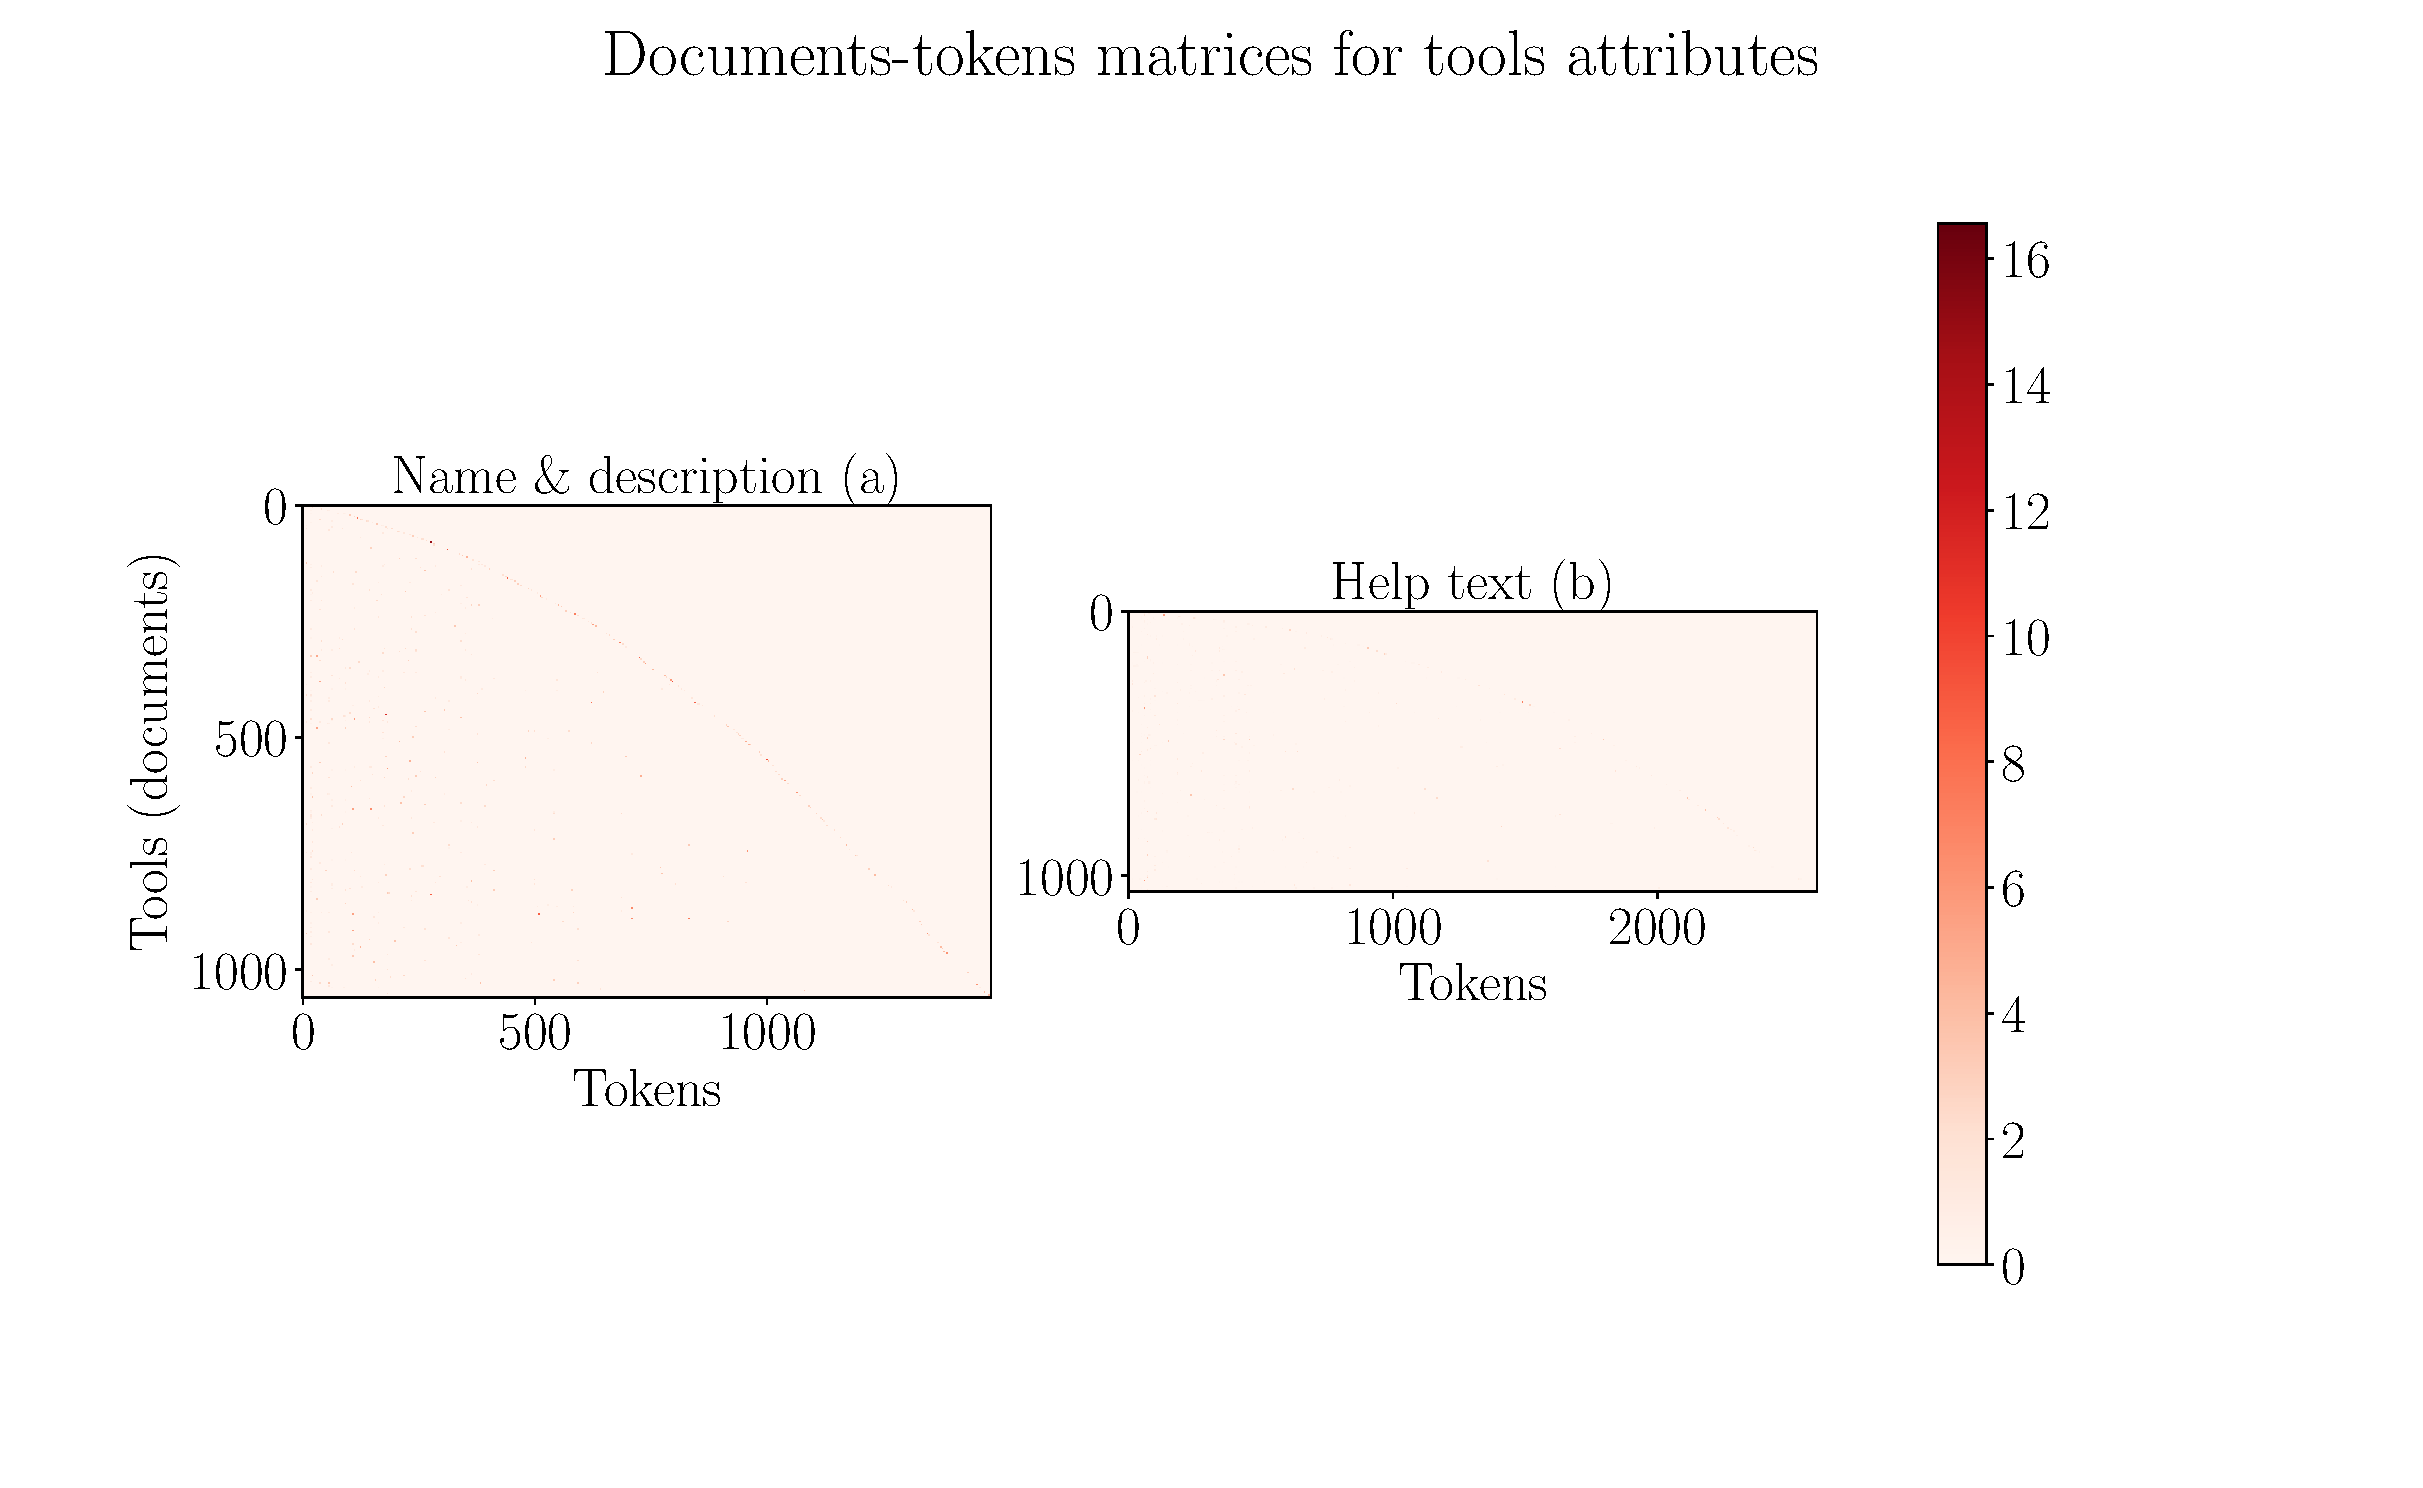
\includegraphics[scale=0.4]{figures/Document_tokens_full_rank.pdf}}
    \caption[Heatmap for documents-tokens matrices]{\textbf{Heatmap for documents-tokens matrices}: The plot shows a heatmap of documents-tokens matrices for name and description and help text attributes. We see that the matrices are sparse containing only few darker spots. The help text matrix is more sparse than name and description matrix as the former contains more number of tokens. We exclude the documents-tokens matrix of input and output file types because we do not intend to find concepts among file types. For the other two matrices, we estimate their dense, lower-rank approximations.}
\end{centering}
\end{figure}

\section{Learn dense vector for a document}
\subsection{Latent semantic indexing}
    It is a mathematical way to learn the hidden (latent) concepts in documents by computing a low-rank representation of a documents-tokens matrix \cite{Foltz1996, Shapiro2000, Landauer1998}. This low-rank matrix is dense (figure 12). We use singular value decomposition ($SVD$) for this decomposition. The optimal rank to which a matrix needs to be decomposed to get the best approximation of the full-rank matrix is empirical in nature. We choose ranks from higher to lower for decomposition and consequently the sum of singular values also decreases with the rank. This decomposition follows the equation:
    
    \begin{equation}
    X_{n \times m} = U_{n \times n} \cdot S_{n \times m} \cdot V_{m \times m}^T
    \end{equation}
    
    where $n$ is the number of documents and $m$ is the number of tokens. $S$ is a diagonal matrix containing the singular values in descending order. It contains the weights of the concepts present in the documents-tokens matrix. The matrices $U$ and $V$ and orthogonal matrices and satisfy:
    
    \begin{equation}
    U^T \cdot U = I_{n \times n}
    \end{equation}
    \begin{equation}
    V^T \cdot V = I_{m \times m}
    \end{equation}
    
\begin{figure}[h]
\begin{centering}
    {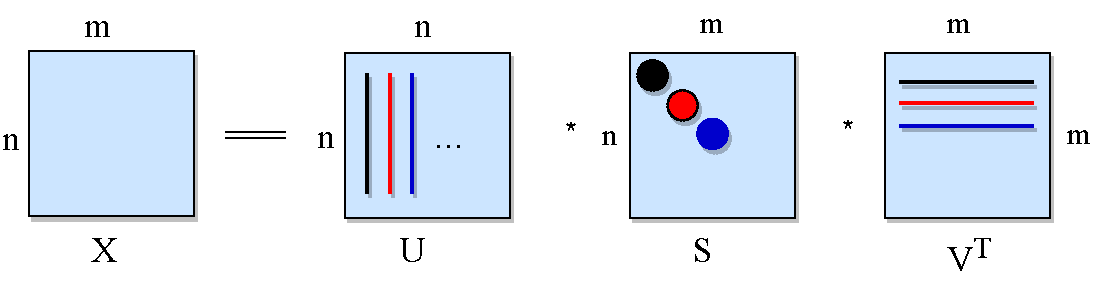
\includegraphics[scale=0.7]{figures/usv.pdf}}
    \caption[Pictorial representation of singular value decomposition]{\textbf{Singular value decomposition}: The image shows that how a matrix is decomposed using singular value decomposition. A matrix $X$ is decomposed into three matrices, $U$, $S$ and $V$. The $k$ ($<m$) most important dimensions are kept and the rest are discarded. The value of $k$ is empirical and can be estimated using optimization taking Frobenius norm as an error function.}
\end{centering}
\end{figure}

Figure 8 explains\footnote{\url{http://theory.stanford.edu/~tim/s15/l/l9.pdf}} how the $SVD$ of a matrix is carried out. The matrix $U$ contains information about how the tokens, arranged along the columns, are mapped to concepts. The matrix $V$ stores information about how the concepts are mapped to documents arranged along the rows.

\subsubsection{Low-rank approximation}
The low-rank approximation of a matrix is important to discard the features which are non-repeating. These features with low scaling factors represent noise and by discarding these unimportant features, we can collect the latent relations present in the documents-tokens matrices. We have seen that our documents-tokens matrices suffer from sparsity and exhibit no relation among tokens. The low-rank approximation deals with these issues. The resulting matrices are dense and contain top singular values (which are higher in magnitude). The singular values which are small (the last entries of the $S$ matrix along the diagonal) are discarded \cite{DBLP:journals/corr/Yang15b}. The low-rank approximation $X_k$ ($k<m$) is computed as:
    \begin{equation}
    X_{n \times m} = U_{k} \cdot S_{k} \cdot V_{k}^T
    \end{equation}
    where $U_{k}$ is the first $k$ columns of $U$, $V_{k}$ is the first $k$ rows and $S$ is the first $k$ singular values. $k$ is an empirical parameter. $X_k$ is called as the rank-k approximation of the full-rank matrix $X$. Figure 10 shows how the rank varies with the sum of singular values for documents-tokens matrices for all the attributes. Figure 11 shows how the fraction of the sum of singular values vary with the fraction of ranks of documents-tokens matrices for all the attributes. The percentage rank is $k \div K$ where $1 <= k <= K$ and $K$ is the original (full) rank of a matrix. By taking fractions, we bring all the three plots from figure 10 into one plot. From figure 11, we can say that if we reduce the ranks of matrices to $70\%$ of the full-rank, we can still capture $\approx 90\%$ of the sum of singular values. The reduction to half of the full-rank achieves $\approx 80\%$ of the sum of singular values. We show the variation for input and output file types in figure 10 and 11 but we do not reduce its rank. That is for completeness.

\begin{figure}[h]
\begin{centering}
    {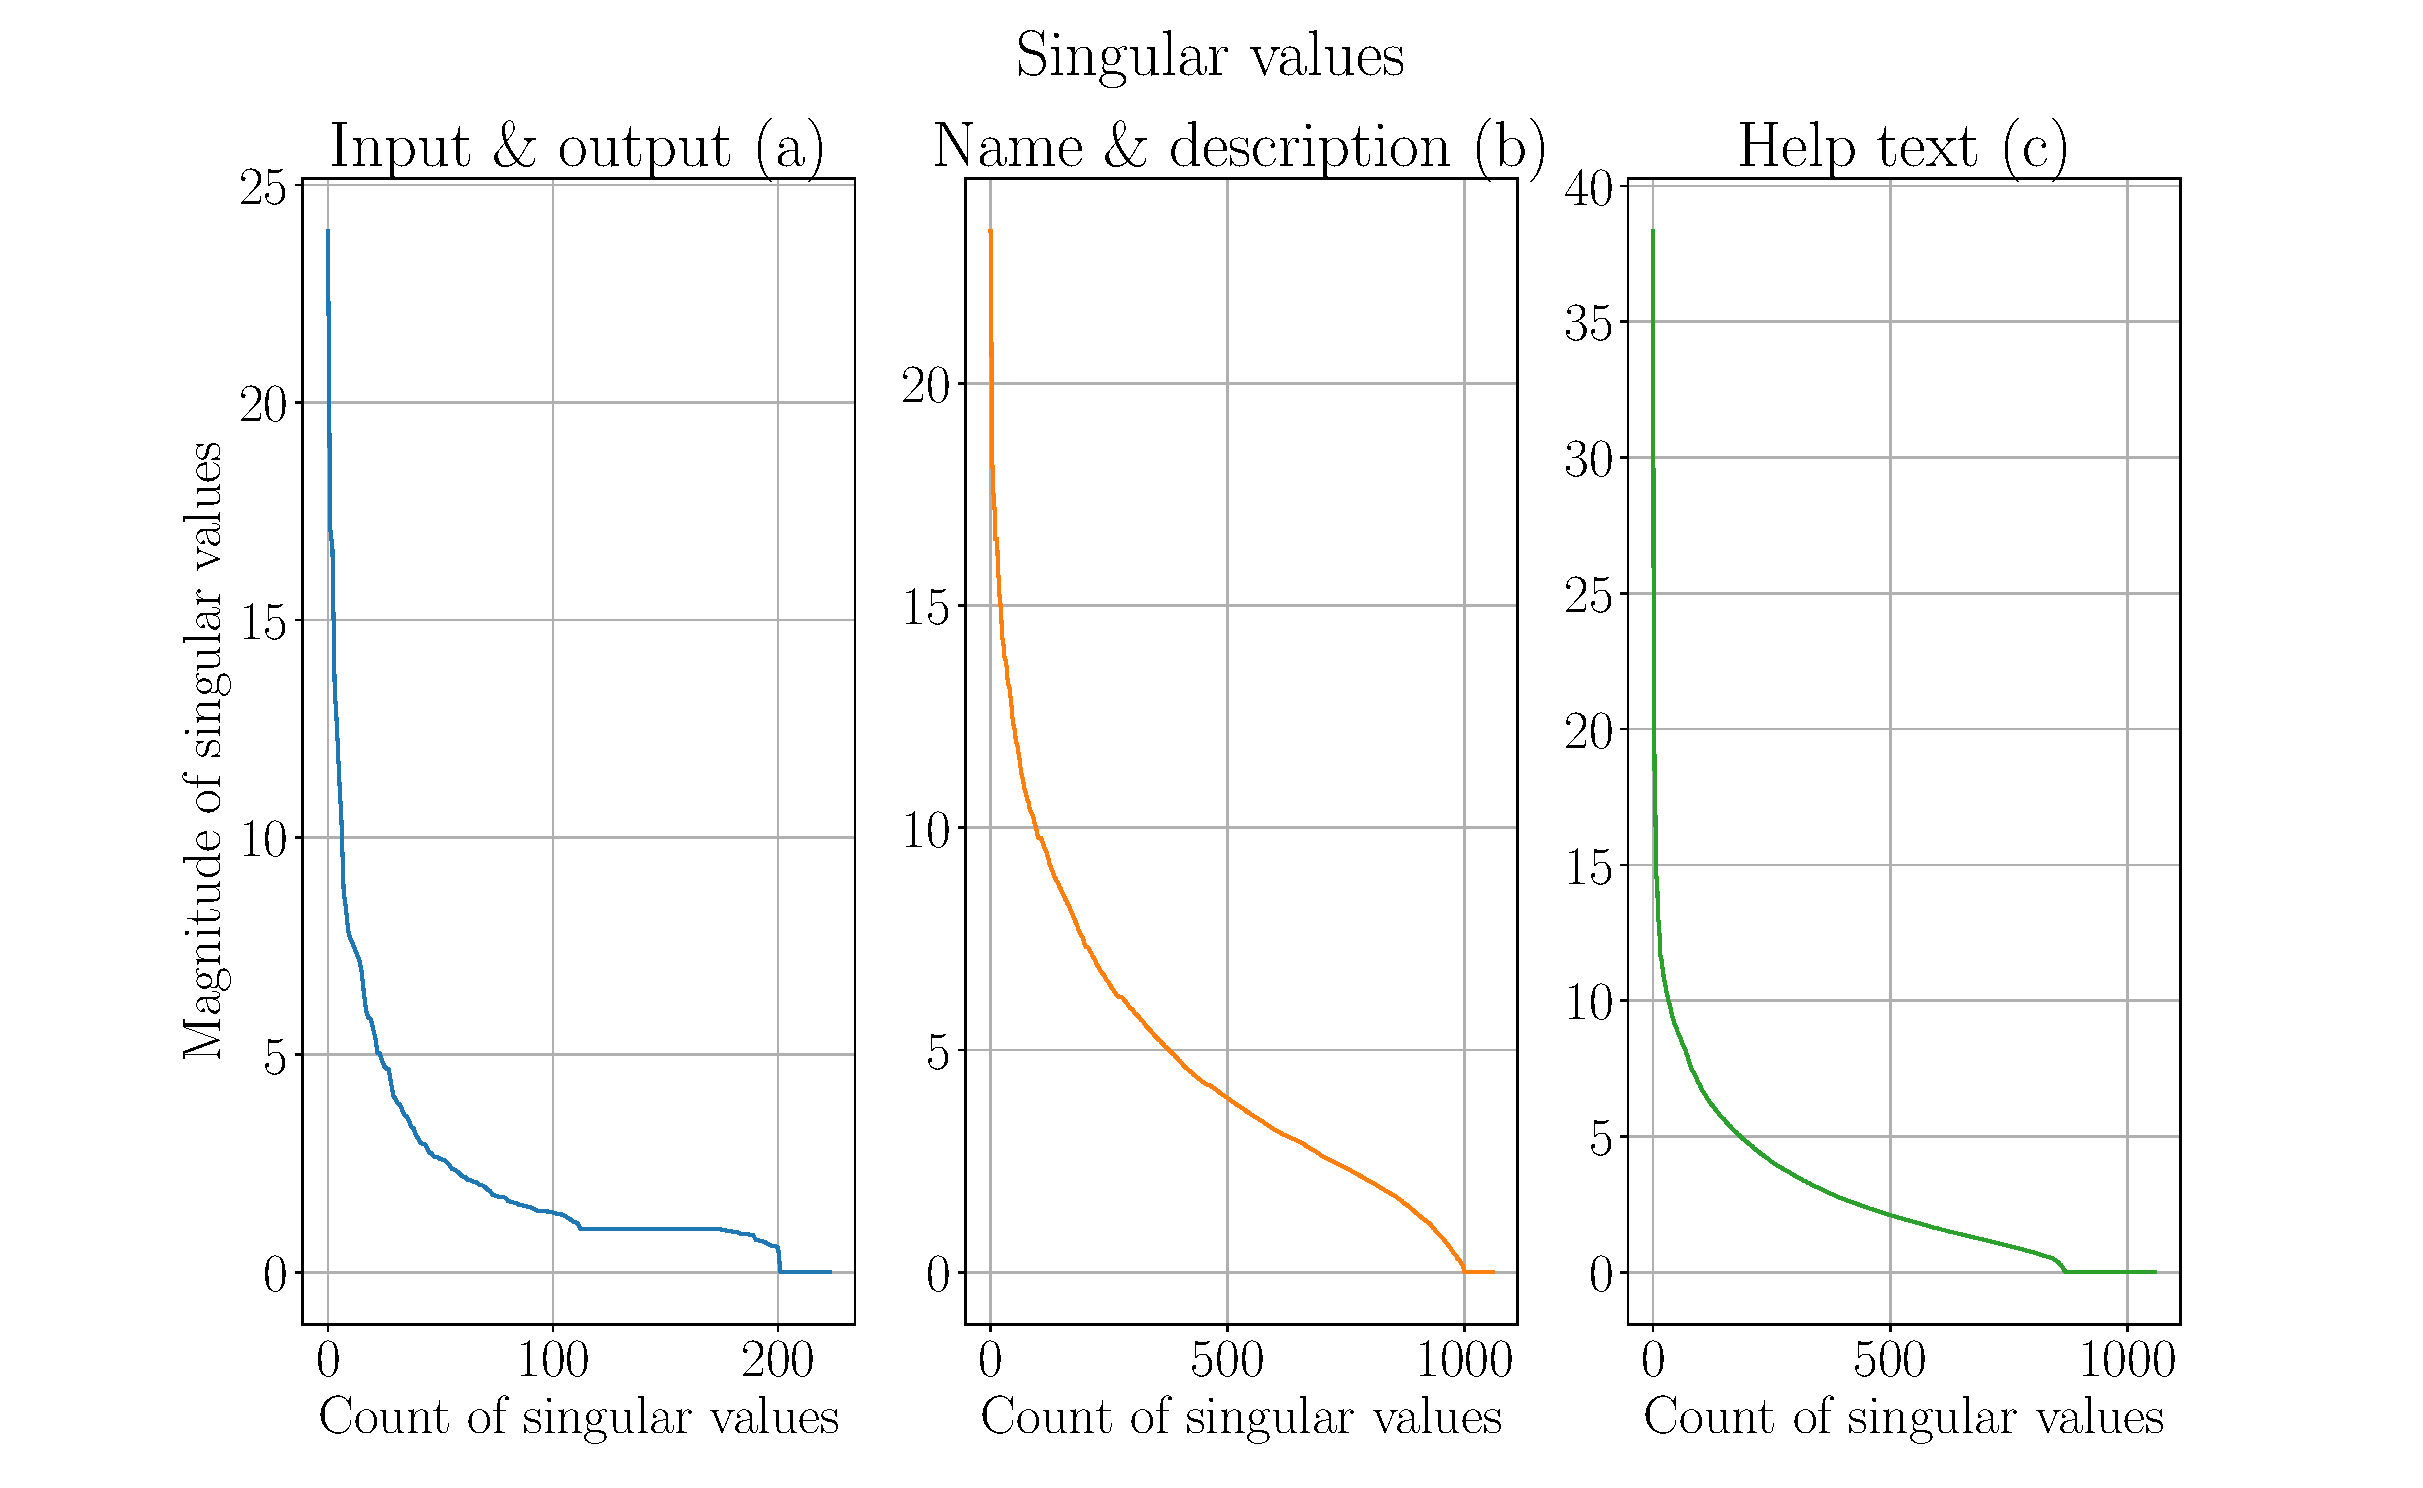
\includegraphics[scale=0.35]{figures/Singular_values.pdf}}
    \caption[Singular values of documents-tokens matrices]{\textbf{Singular values of the documents-tokens matrices}: The plot shows singular values computed using singular value decomposition (equation 5). The diagonal matrix $S$ contains these singular values sorted in descending order. We can see that in (a), (b) and (c) that very few singular values have higher mangnitude and most of the singular values are smaller.}
\end{centering}
\end{figure}

\begin{figure}[h]
\begin{centering}
    {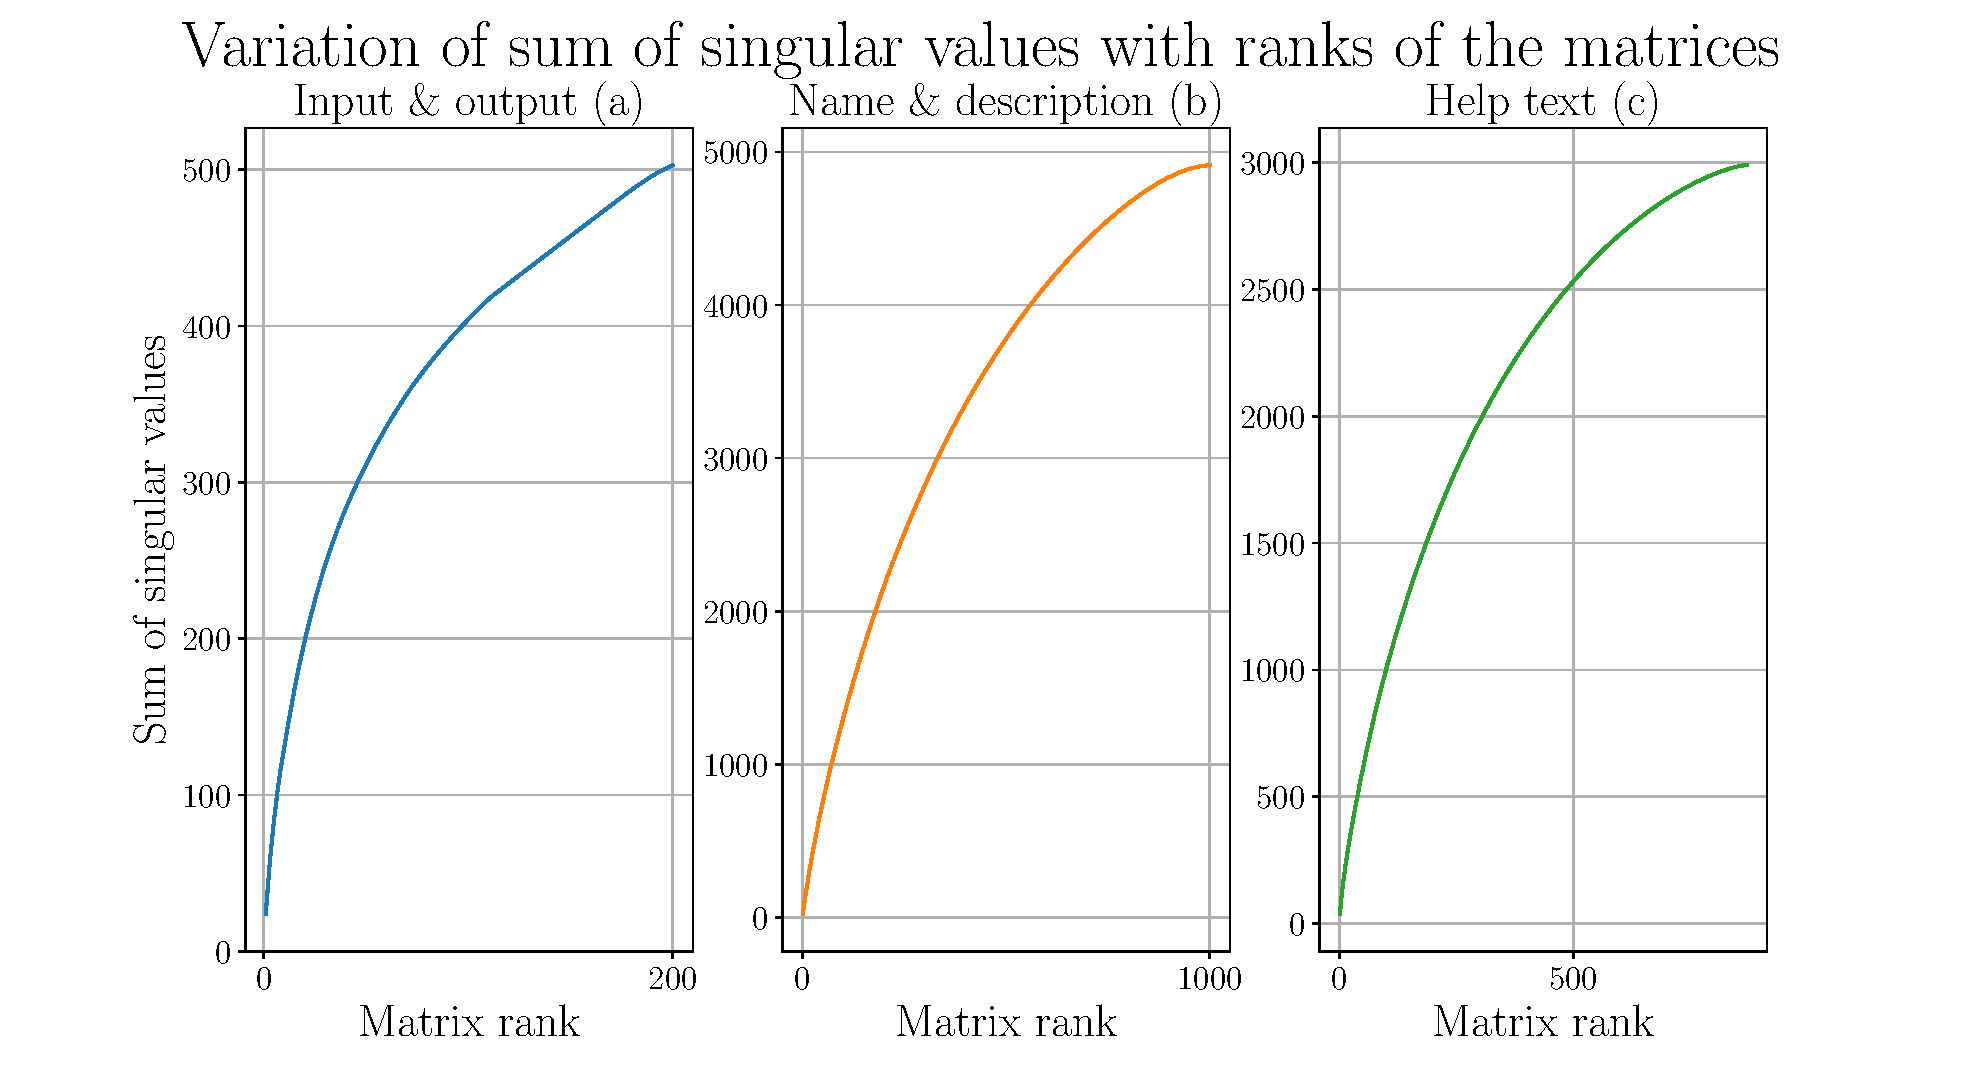
\includegraphics[scale=0.45]{figures/Sum_singular_ranks.pdf}}
    \caption[Singular values of documents-tokens matrices with their respective ranks]{\textbf{Sum of singular values with matrix rank}: The plot shows an easier way to see how the sum of singular values varies with a documents-tokens matrix rank for the three attributes. Here the (a), (b) and (c) show separately this variation as the ranks of these matrices and sum of singular values differ.}
\end{centering}
\end{figure}

\begin{figure}[h]
\begin{centering}
    {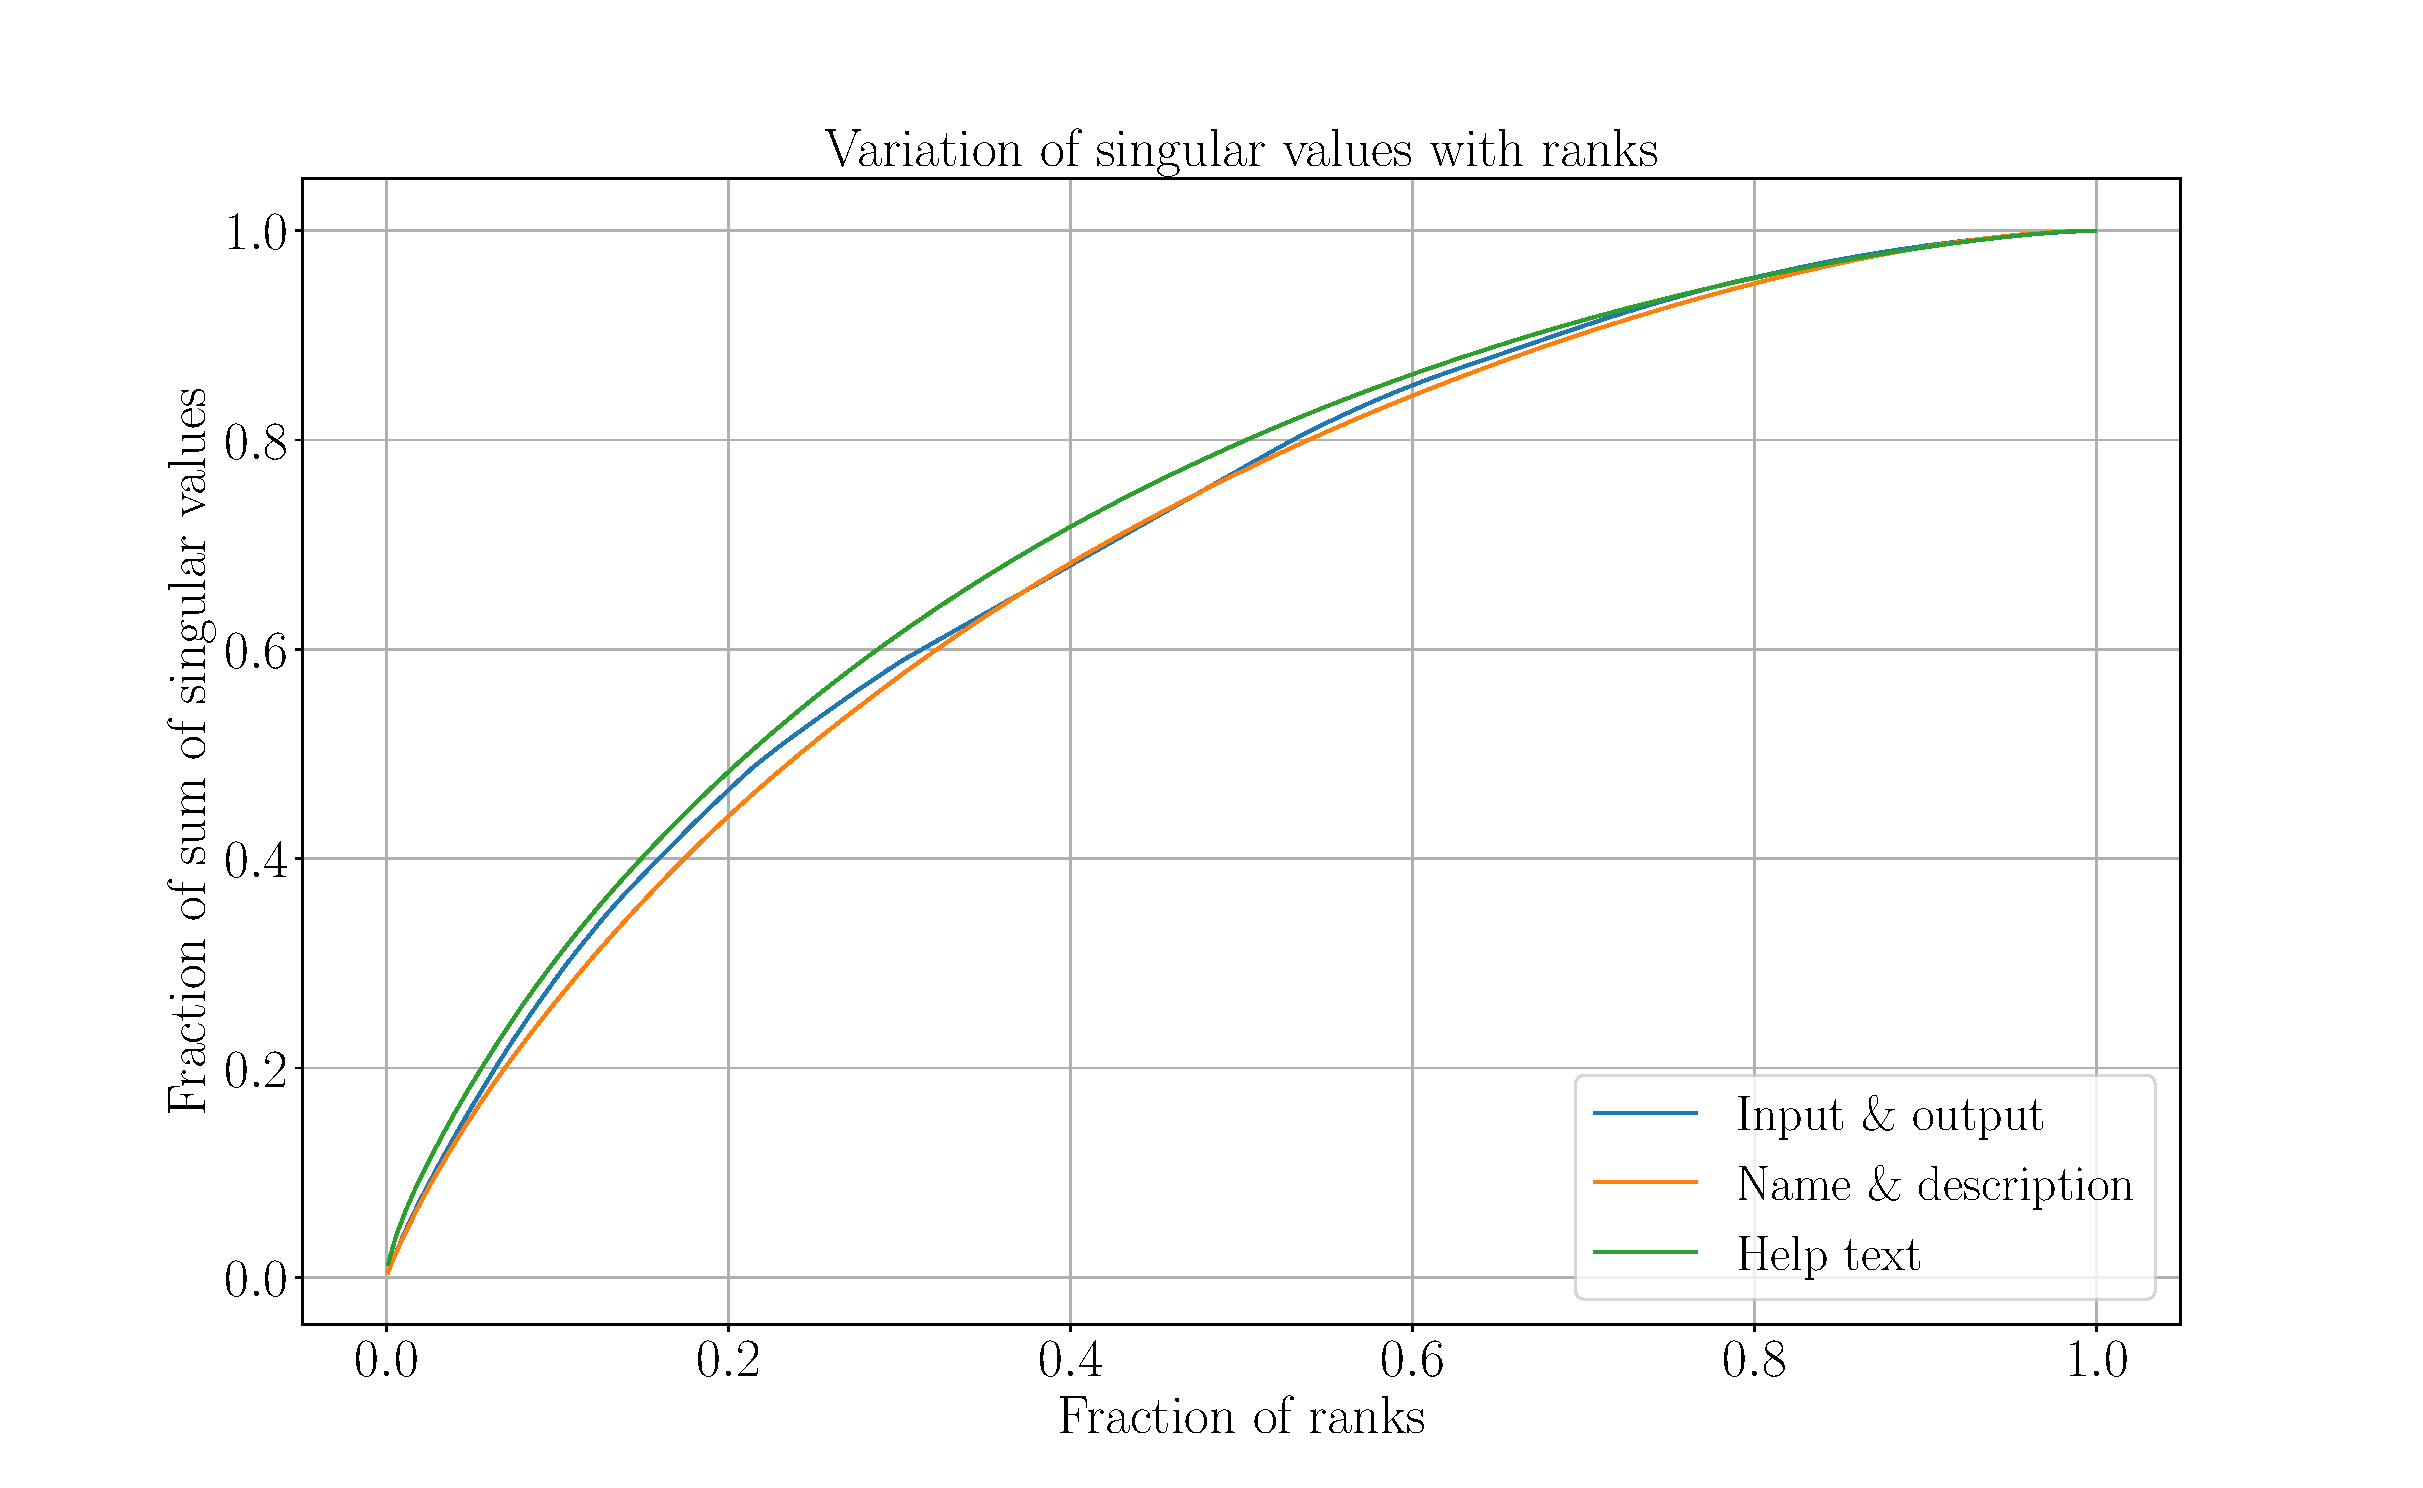
\includegraphics[scale=0.4]{figures/Fraction_ranks_singular_values.pdf}}
    \caption[The variation of fraction of ranks of documents-tokens matrices with the fraction of sum of singular values]{\textbf{The variation of fraction of ranks of documents-tokens matrices with the fraction of sum of singular values}: This plot merges the results of the figure 10 into one plot. As the ranks of document-term matrices and sum of singular values vary, we convert them to respective percentages. $rank_{fraction} = \frac{k}{N}$ where $k$ is the reduced rank and $N$ is the full-rank of a matrix For example $0.2$ on the rank axis (x-axis) means $20\%$ of the original rank of a matrix. Similarly, y-axis shows the fraction of the sum of all singular values $ sum_{fraction} = \frac{\sum_{i=1}^k}{\sum_{i=1}^K}$ where $K$ is the number of all singular values.}
\end{centering}
\end{figure}

We reduce the rank of the original documents-tokens matrices and compute the dense and low-rank approximations. Figure 12 shows the low-rank matrices for name and description and help text attributes. To compute this, we use only $5\%$ of the full-rank. We can compare it with figure 7 and verify that it is more dense than figure 7. In these low-rank matrices, we get dense vector representations for documents along the rows. In each matrix, each row contains a vector for one document. Using these documents vectors, we can compute the correlation or similarity using a similarity measure. There are multiple similarity measures which can be used like euclidean distance, cosine similarity, manhattan distance, jaccard index and many more. In our case, we use cosine angle similarity for name and description and help text and jaccard index for input and output file types to compute the correlation between vectors. We get a positive real number between $0.0$ and $1.0$ as similarity score between a pair of vectors specifying how similar they are. The higher the score, higher is the similarity. Computing this similarity for all the documents gives us a similarity matrix $S_{n \times n}$ where $n$ is the number of documents (tools). This square, symmetric matrix is called as similarity or correlation matrix. We compute three such matrices, each corresponding to one attribute (input and output file types, name and description and help text).
  
\begin{figure}[h]
\begin{centering}
    {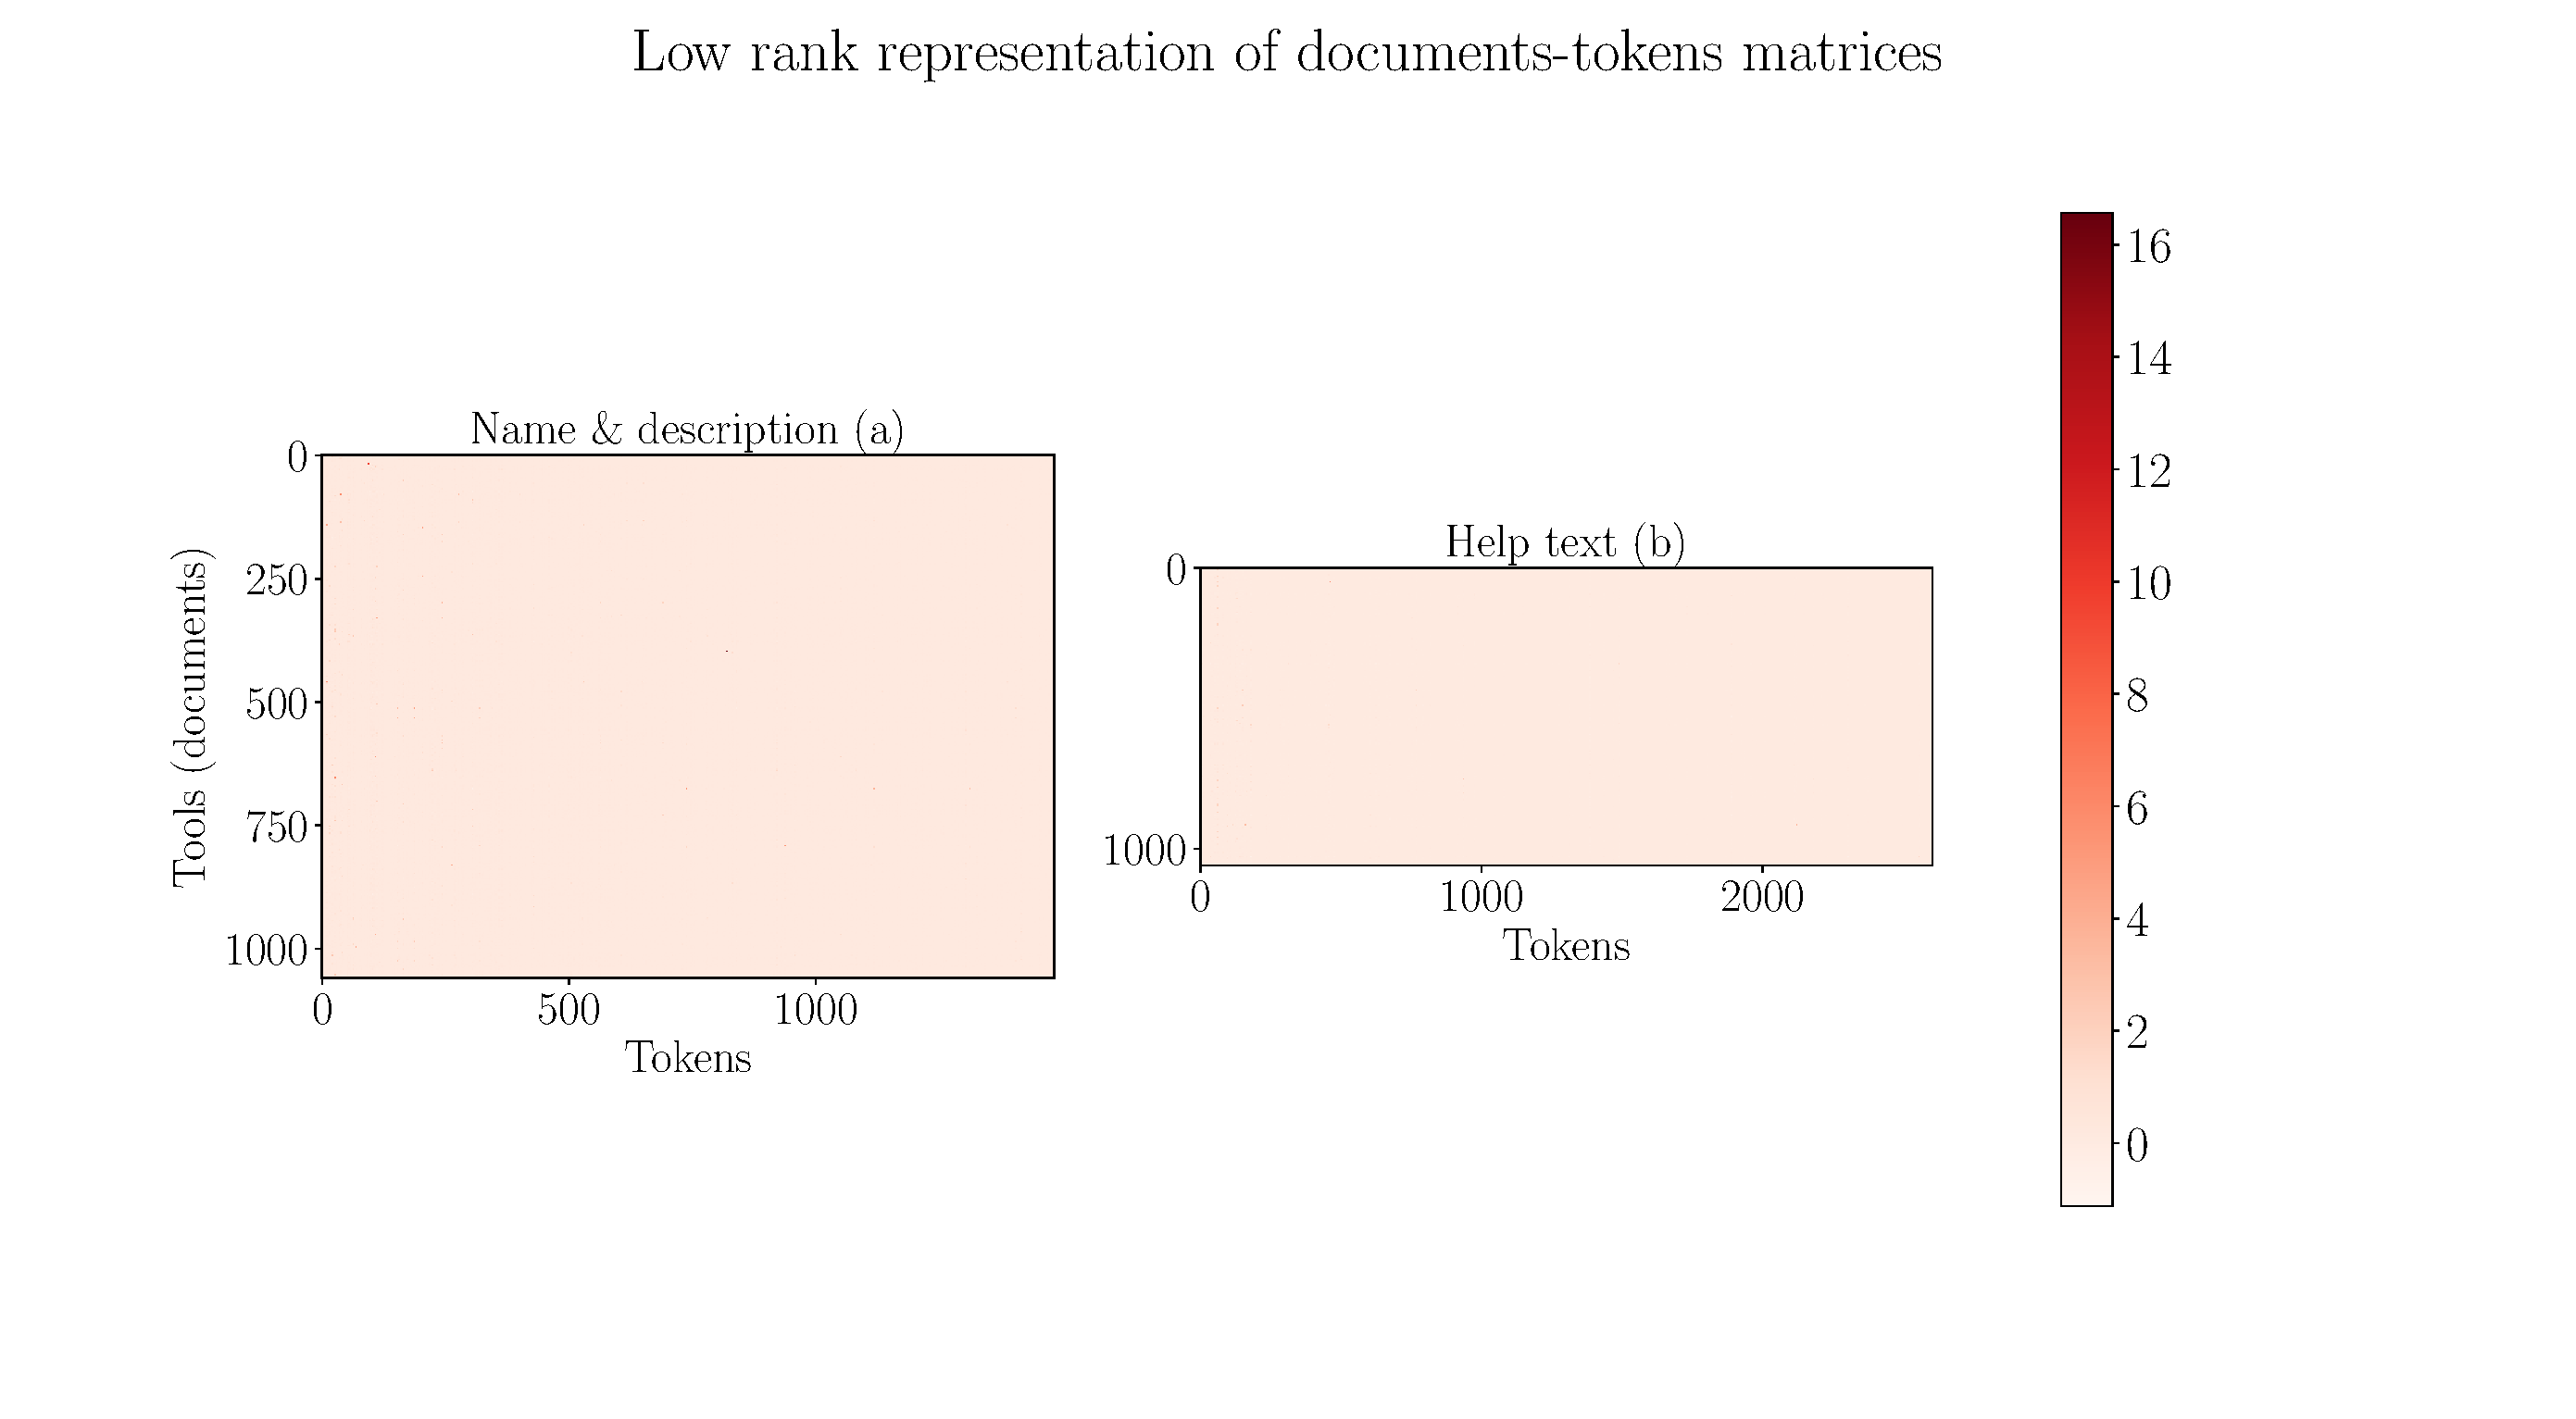
\includegraphics[scale=0.35]{figures/Document_tokens_low_rank.pdf}}
    \caption[Low-rank representations of documents-tokens matrices]{\textbf{Low-rank representations of documents-tokens matrices}: The heatmap shows the low-rank ($5\%$ of full-rank) representations of documents-tokens matrices for name and description and help text. These matrices are more dense compared to figure 7 which shows these matrices corresponding to the full-rank representations.}
\end{centering}
\end{figure}

\subsection{Paragraph vectors}
Using latent semantic indexing (LSI), we learned dense vectors to represent each document. It learns better vector representations for documents compared to using full-rank documents-tokens matrices. One main limitation is to assess the quantity by which we need to lower the rank of a matrix in order to find the optimal results. There are ways to find the optimal reduced rank by optimizing the Frobenius norm but it is not simple. We would see in the analysis section that the similar tools for a tool are more dominated by the scores shared by the input and output file types. Due to this issue, the tools which are similar in their functions do not get pushed up in the ranking ladder. To avoid these limitations, we use an approach known as $doc2vec$ (document to vector) \cite{DBLP:journals/corr/LeM14}. It learns a dense, fixed-size vectors for each document using neural networks. These vectors are unique in a way that captures the semantics present in the documents. The documents which share similar context are represented by similar vectors. When we compute cosine distance between these vectors sharing similar context, we get a higher number (closer to 1.0). It allows the documents to have variable lengths.


\subsubsection{Approach}
Paragraph vectors approach learns vector representations for all the words present in a set of documents. The words which are used in a similar context have similar vectors. For example, words like "data" and "dataset" which are used, in general, in similar contexts have are represented by vectors that are close. The vector representations of words in a document are learnt by maximizing the following equation:

\begin{equation}
\frac{1}{T} \cdot \sum_{t=k}^{T-k} \log p(w_t|w_{t-k,...,t+k})
\end{equation}

where $T$ is the total number of words in a document, $k$ is the window size. We take a few words which make a context and using this context we try to predict each word. The probability $p$ is computed using a softmax classifier and backpropagation is used to compute the gradient and the vectors are optimized using stochastic gradient descent. To learn paragraph vectors, in addition to using words vectors, paragraph vectors are also used to learn the probability of the next words in a context. The paragraph and word vectors are averaged or concatenated to make a classifier which predicts next words in a context. There are two ways how to choose a context.

\begin{itemize}
\item Distributed memory: In this approach of learning paragraph vectors, fixed length window of words are chosen and paragraph and word vectors are used to predict the words in this context. The words vectors are shared across all the paragraphs (documents) and paragraph vector is unique to each paragraph.

\begin{figure}[h]
\begin{centering}
    {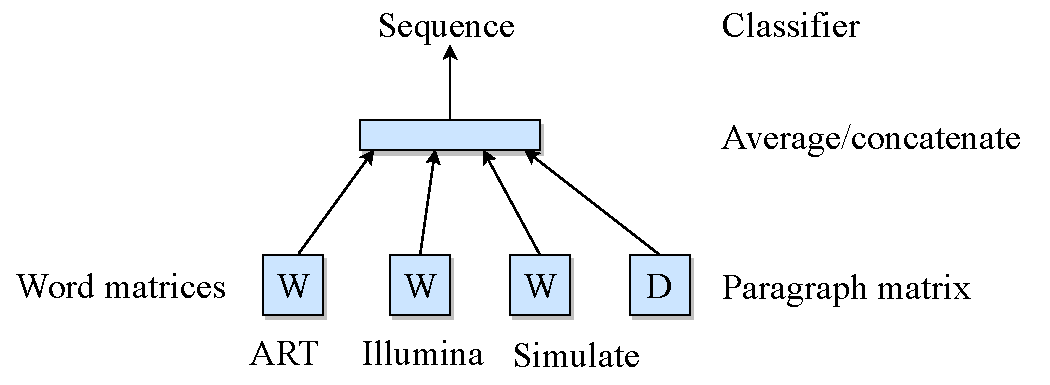
\includegraphics[scale=0.7]{figures/dm_pv.pdf}}
    \caption[Distributed memory approach for paragraph vectors]{\textbf{Distributed memory approach for paragraph vectors}: This image shows a mechanism for learning paragraph (document) vectors. $W$ is a word matrix where each word is represented by a vector. $D$ is a paragraph matrix where each paragraph (document) is represented by a vector. The word vectors are shared across all paragraphs (documents) but not the paragraph vectors. The three words "Art", "Illumina" and "Simulate" represent a context. The average or concatenated words and paragraph vectors are used to predict the "Sequence" word.}
\end{centering}
\end{figure}

\item Distributed bag of words: In this approach, words are randomly extracted from the paragraphs and from this set of words, a word is chosen randomly and predicted using the paragraph vectors. No order is followed in choosing words.
\end{itemize}

\begin{figure}[h]
\begin{centering}
    {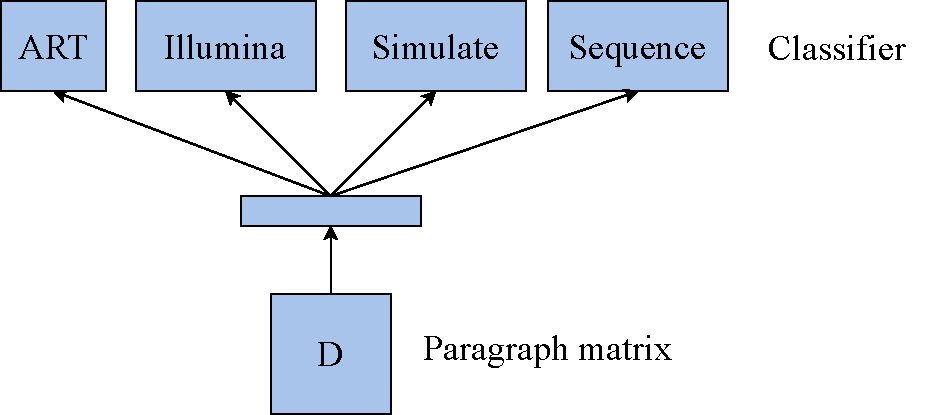
\includegraphics[scale=0.7]{figures/dbow_pv.pdf}}
    \caption[Distributed bag-of-words approach for paragraph vectors]{\textbf{Distributed bag-of-words approach for paragraph vectors}: This image shows how only paragraph vectors are learned by predicting a random word chosen from a randomly selected set of words. In this approach, the order of the words does not matter.}
\end{centering}
\end{figure}

The figures 13 and 14 are inspired from the original work - 
Distributed Representations of Sentences and Document\footnote{\label{pv}\url{https://arxiv.org/abs/1405.4053}}. The second form of learning paragraph vectors is simple and we use it to learn documents (paragraphs) vectors for name and description and help text attributes. We learn only the paragraph vectors which makes it less computationally expensive \cite{DBLP:journals/corr/LeM14} as the number of parameters is less compared to the distributed memory model which learns word vectors as well. The number of parameters in distributed bag-of-words is $\approx N \times z$ where $N$ is the number of paragraphs (documents) and $z$ is the dimensionality of each vector.

\section{Similarity measures}
From latent semantic analysis and paragraph vectors approaches, we generate vectors for the documents that belong to the three attributes. To find similarity between a pair of vectors, we can apply some similarity measures to get a similarity score. This score quantifies how much similar a pair of documents are. In this work, we use two similarity measures - cosine similarity and jaccard index. Both of these measures return a positive real number between $0$ and $1$ as a similarity score.

\subsection{Cosine similarity}
It calculates the cosine angle value between a pair of document vectors. Let's say we have two vectors, $x$ and $y$. We can write:
\begin{equation}
x \cdot y = |x| \cdot |y| \cdot \cos{\theta}
\end{equation}

\begin{equation}
\cos{\theta} = \frac {x \cdot y}{|x| \cdot |y|} 
\end{equation}

where $|x|$ is the norm of the vector $x$. If the norm is $0$, we use $0$ for the value of $\cos{\theta}$. $x \cdot y$ is the dot product of vectors $x$ and $y$. The values emitted by this similarity follows a natural progression that if the documents are dissimilar, then it is $0$ and if completely similar, it is $1.0$. Otherwise it lies between $0.0$ and $1.0$. This score can also be understood as a kind of probability of similarity between a pair of documents\footnote{\url{https://nlp.stanford.edu/IR-book/html/htmledition/dot-products-1.html}}.


\subsection{Jaccard index}
Jaccard index is a measure of similarity between two sets of entities and is given by the equation:

\begin{equation}
j = \frac{A \cap B}{A \cup B}
\end{equation}
where $A$ and $B$ are two sets. $\cap$ is the number of entities present in both the sets and $\cup$ is the sum of unique entities present in sets $A$ and $B$ \cite{Ivchenko1998}. We use this measure to compute the similarity between two tools based on their file types. For example, "LinearRegression" has 3 file types: $tabular$, $input$ and $pdf$. Another tool "LDAAnalysis" has $tabular$ and $txt$ as file types. The jaccard index for this pair of tools would be:

\begin{equation}
j = \frac{Length[(tabular, input, pdf) \cap (tabular, txt)]}{Length[(tabular, input, pdf) \cup (tabular, txt)]} = \frac{1}{4} = 0.25
\end{equation}

\section{Optimization}
We get similarity matrices after applying similarity measures on the document vectors, one each for input and output file types, name and description and help text attributes. These matrices have the same dimensions ($N \times N$, $N$ is the number of documents (tools)). To combine these matrices, one simple idea would be to take an average of the corresponding rows of similarity scores from the matrices. Doing this, we get combined similarity scores of one document (tool) with all other documents (tools). Iterating this process for all the documents would give us a similarity matrix which contains similarity scores of documents with all the other documents. The diagonal entries of this matrix would be $1.0$ and all the other entries would be a positive real number between $0.0$ and $1.0$. Another way to find the combination is to learn the weights on the rows from three matrices and then combine them to obtain optimal similarity scores for a document (tool). The weights are positive real numbers between $0.0$ and $1.0$ and for each row, they sum up to $1.0$. Instead of using fixed importance factors (weights) of $1/3$ ($3$ is the number of matrices), we use an optimization technique to find these real numbers and then combine the matrices by multiplying with these weights to obtain a weighted average optimal similarity matrix.

\begin{equation}
S_k^{optimal} = w^k_{io} \cdot S^k_{io} +  w^k_{nd} \cdot S^k_{nd} + w^k_{ht} \cdot S^k_{ht}
\end{equation}

where $w$ is a positive, real number and satisfy $w^k_{io} + w^k_{nd} + w^k_{ht} = 1$. 
$S^k_{io}$, $S^k_{nd}$ and $S^k_{ht}$ are the similarity scores (corresponding matrix rows) for $k^{th}$ tool corresponding to input and output file types, name and description and help text attributes respectively. Similarity scores $S$ has a dimensionality of $1 \times N$ where $N$ is the number of tools (documents). Each similarity score among a set of documents (tools) is independent of one another. We already have these similarity scores and need to learn the importance weights to compute the optimal similarity scores. We use gradient descent optimizer to learn the weights by minimizing an error function. To define an error function, we need to set true values where we intend to reach and then we compute mean squared error. If we look at the similarity measure, we see that the maximum similarity between a pair of documents can be $1.0$. Hence, the ideal similarity scores for a document with any other document can be at most $1.0$.

\begin{equation}
S_{ideal} = [ 1.0, 1.0, ...., 1.0 ]
\end{equation}
where $S_{ideal}$ is the ideal similarity scores for one document against all the other documents. $S_{ideal}$ has a dimensionality of $1 \times N$ where $N$ is the number of documents. Using the ideal score, we can compute the mean squared error we accrue for all the similarity scores from the three attributes separately. After computing the error, we can verify which attribute is closer to the ideal score and which are not. The attributes which measure lower error get higher weights and those which score higher error get lower weights. The next section elaborates how we use gradient descent to do the optimization.

\subsection{Gradient descent}
Gradient descent is a popular algorithm for optimizing an objective function with respect to its parameters. The parameters are the entities which we want to learn. In our case, these are the weights. The algorithm minimizes an error function. The error function which we define is the mean squared error:

\begin{equation}
Error^k_{io}(w_{io}) = \frac{1}{N - 1} \cdot \sum_{t=1}^{N-1} (w_{io} \cdot S^t_{io} - S_{ideal}) ^ 2
\end{equation}

\begin{equation}
Error^k_{nd}(w_{nd}) = \frac{1}{N - 1} \cdot \sum_{t=1}^{N-1} (w_{nd} \cdot S^t_{nd} - S_{ideal}) ^ 2
\end{equation}

\begin{equation}
Error^k_{ht}(w_{ht}) =  \frac{1}{N - 1} \cdot \sum_{t=1}^{N-1} (w_{ht} \cdot S^t_{ht} - S_{ideal}) ^ 2
\end{equation}

\begin{equation}
Error^k(w) =  \frac{1}{N - 1} \cdot \sum_{t=1}^{N-1} (w \cdot S^t - S_{ideal}) ^ 2
\end{equation}

\begin{equation}
\argmin_w Error^k(w) 
\end{equation}

\begin{equation}
\sum_{i=1}^{3} w_i = 1
\end{equation}

$Error$ is an error vector - $<Error_{io}, Error_{nd}, Error_{ht}$, $w$ is a weight vector - $<w_{io}, w_{nd}, w_{ht}>$ and $S$ similarity scores vector - $<S_{io}, S_{nd}, S_{ht}>$. $io$, $nd$ and $ht$ refer to input and output file types, name and description and help text for $Error$, $w$ and $S$. All these vectors are averaged over $N-1$ where $N$ is the number of documents (tools). We take $N-1$ in order to remove the concerned tool's similarity score with itself. To minimize the equation $20$ under the constraint given by equation $21$ where $0 \leq w_i \leq 1$ and $3$ is the number of attributes, we need to compute the gradient of the error function. The gradient specifies the rate of change of error with respect to the weights.

\begin{equation}
Gradient^k(w) = \frac{\partial Error^k}{\partial w} =  \frac{2}{N - 1} \cdot \sum_{t=1}^{N-1} (w \cdot S^t - S_{ideal}) \cdot S^t
\end{equation}

$Gradient$ is also a vector - $<Gradient_{io}, Gradient_{nd}, Gradient_{ht}>$. Using the gradient vector, we can update the weights. For this, we need to set the learning rate. Finding the right learning rate is important because a higher value can diverge the gradient descent and a lower value can slow down the learning and it could take a lot of time to converge to the minimum of the error function. For each iteration of gradient descent, we employ time-based decay of learning rate.

\begin{equation}
w^k = w^k - \eta \cdot {Gradient(w^k)}
\end{equation}
where $\eta$ is the learning rate.

\subsection{Learning rate decay}
Finding good learning rates forms an important part of the gradient descent optimization. If the learning rate is high, it poses a risk of optimizer divergence. On the other hand, if it is small, the optimizer can take a long time to converge. Both these situations are underisable. But, we can avoid these drawbacks by starting out with a small learning rate and gradually decrease it over the iterations. It is called as a time-based decay of the learning rate \cite{articleRuderS}.

\begin{equation}
lr^{t+1} = \frac{lr^t}{( 1 + ( decay * iteration ) )}
\end{equation}
where $lr^{t+1}$ and $lr^t$ are the learning rates for $t+1$ and $t$ iterations, $decay$ controls how steep or flat the learning rate curve is and $iteration$ is the gradient descent iteration number. A higher value of decay makes the learning rate curve steep as the learning rate drops quickly. A lower value can make the curve flat which can slow down the learning.

\begin{figure}[h]
\begin{centering}
    {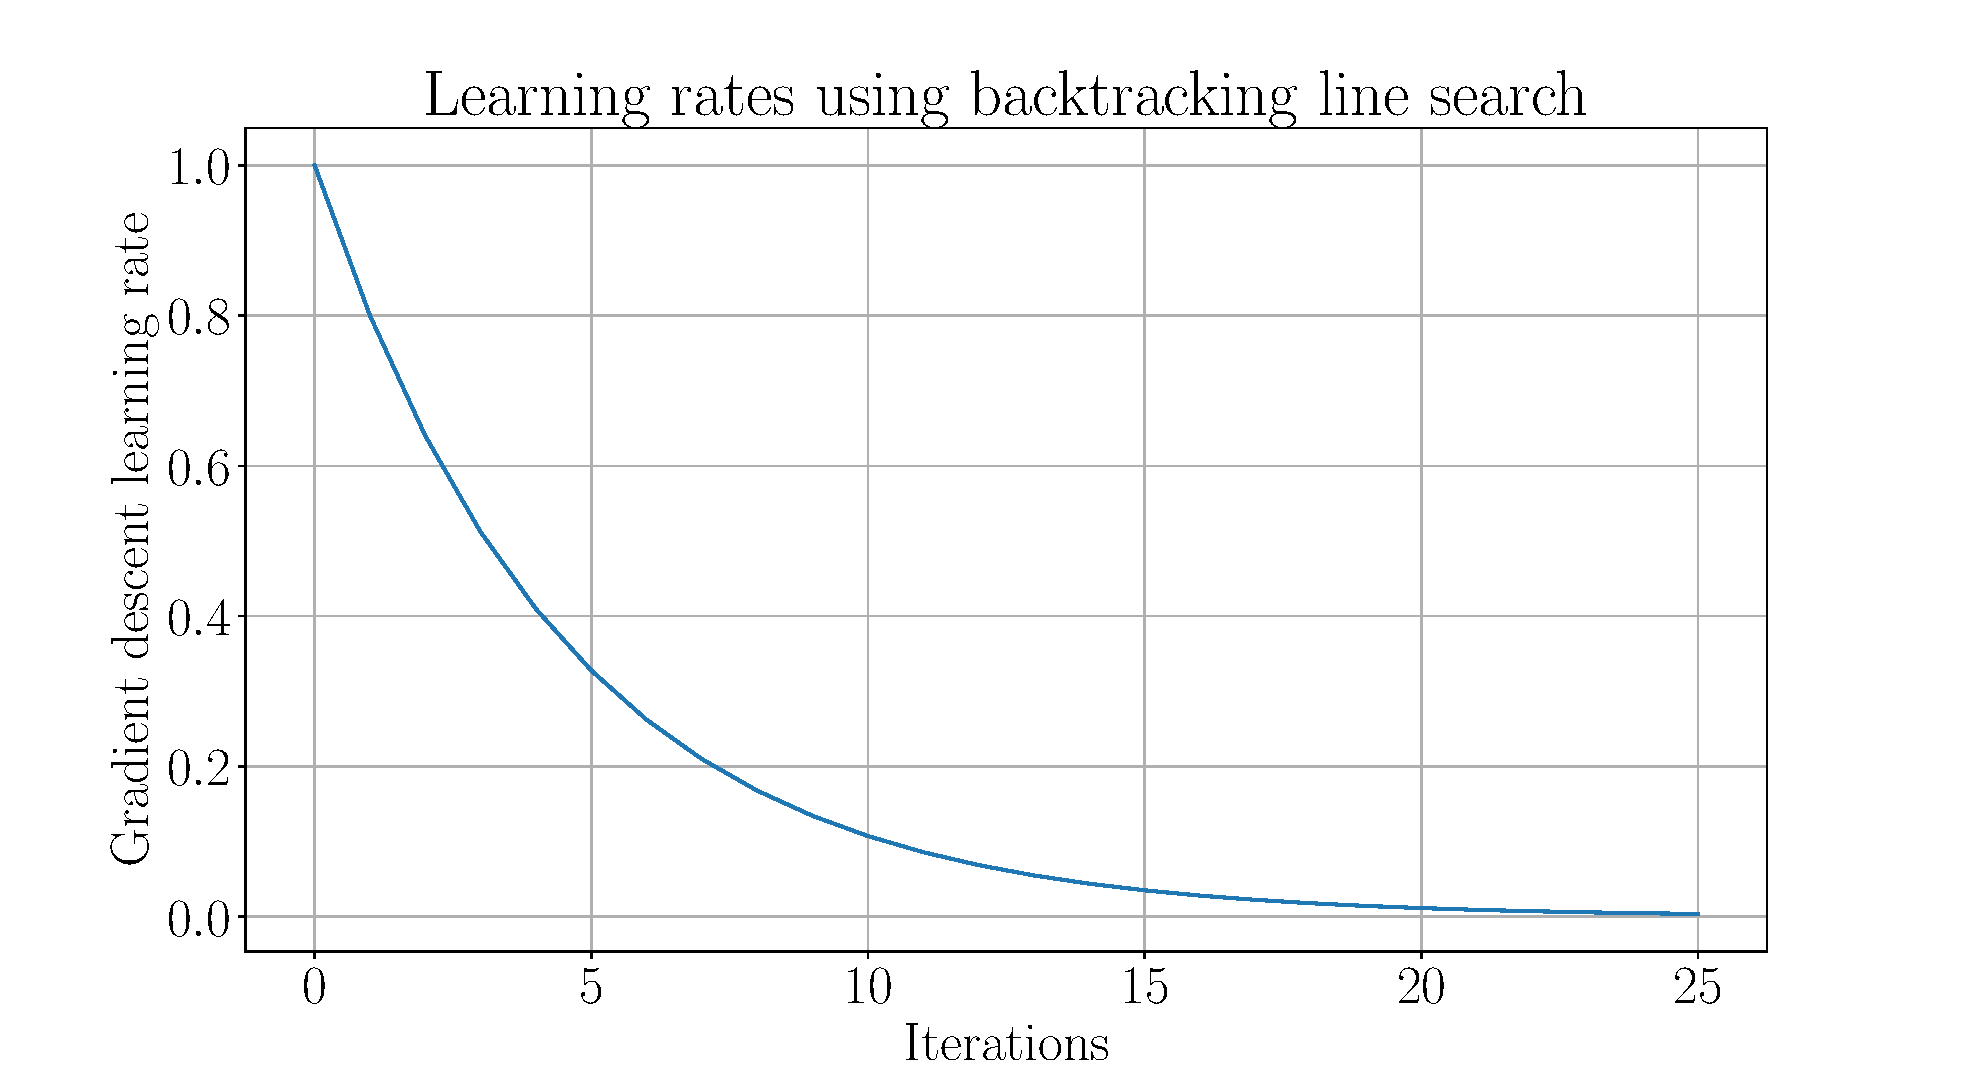
\includegraphics[scale=0.35]{figures/Learning_rates.pdf}}
    \caption[Decay of learning rate for gradient descent optimizer]{\textbf{Decay of learning rate for gradient descent optimizer}: The plot shows how the learning rate for gradient descent evolves with iterations. It starts with a small value and decreases gradually over time. It is essential to have learning rates which neither drops too quickly or too slowly. Both of these ways can lead to divergence or slow convergence of the optimizer.}
\end{centering}
\end{figure}

\subsection{Weight update}
\subsubsection{Momentum}
To reach the minimum point of our convex error function (equation 20), we need to go down continuously without being blocked at the saddle points. These saddle points are where the derivative of a function is zero. Adding a momentum term to the weight parameter, we expect to avoid the local minima and should be able to converge to the lowest point quickly. It gives the necessary push to keep going down the convex error function by adding a fraction of the previous step update to the current update \cite{articleRuderS, Sutskever}. We compute the weight parameter update for each iterations using:

\begin{equation}
update_{t+1} = \gamma \cdot update_{t} - \eta \cdot Gradient(w^t)
\end{equation}

\begin{equation}
w_{t+1} = w_t + update_{t+1}
\end{equation}

where $update_{t+1}$ is the update for changing the weight parameter for the current iteration $t+1$. $update_{t}$ is the previous iteration update. $\eta$ is the learning rate and $Gradient$ is with respect to the weight parameter $w_t$. 

\subsubsection{Nesterov’s accelerated gradient}
The inclusion of momentum is useful to get necessary advance towards finding the minimum of the error function. However, the speed of going down the slope of the error function should become less if there is a possibility of change in gradient direction. In this situation, the speeding up can be avoided by estimating the forthcoming gradient (gradient for the next step) and then correcting it \cite{Botev}. We update the weight parameter using the following equations:

\begin{equation}
update_{t+1} = \gamma \cdot update_t - \eta \cdot Gradient(w_t + \gamma \cdot update_t)
\end{equation}

\begin{equation}
w_{t+1} = w_t + update_{t+1}
\end{equation}

\subsubsection{Gradient verification}
We compute gradient using equation 21 and use it to update our weight parameters. To verify that the computed gradient is correct, we can approximate this gradient using the error function which we formulated in equation 19.

\begin{equation}
Gradient(w) = \frac{\partial Error}{\partial w} \approx \frac{Error(w + \epsilon) - Error(w - \epsilon)}{2 \cdot \epsilon} 
\end{equation}
where $\epsilon$ is a very small number ($\approx10^{-4}$). Figure 16 shows the difference of the actual and approximated gradients for all the three attributes.

\begin{figure}[h]
\begin{centering}
    {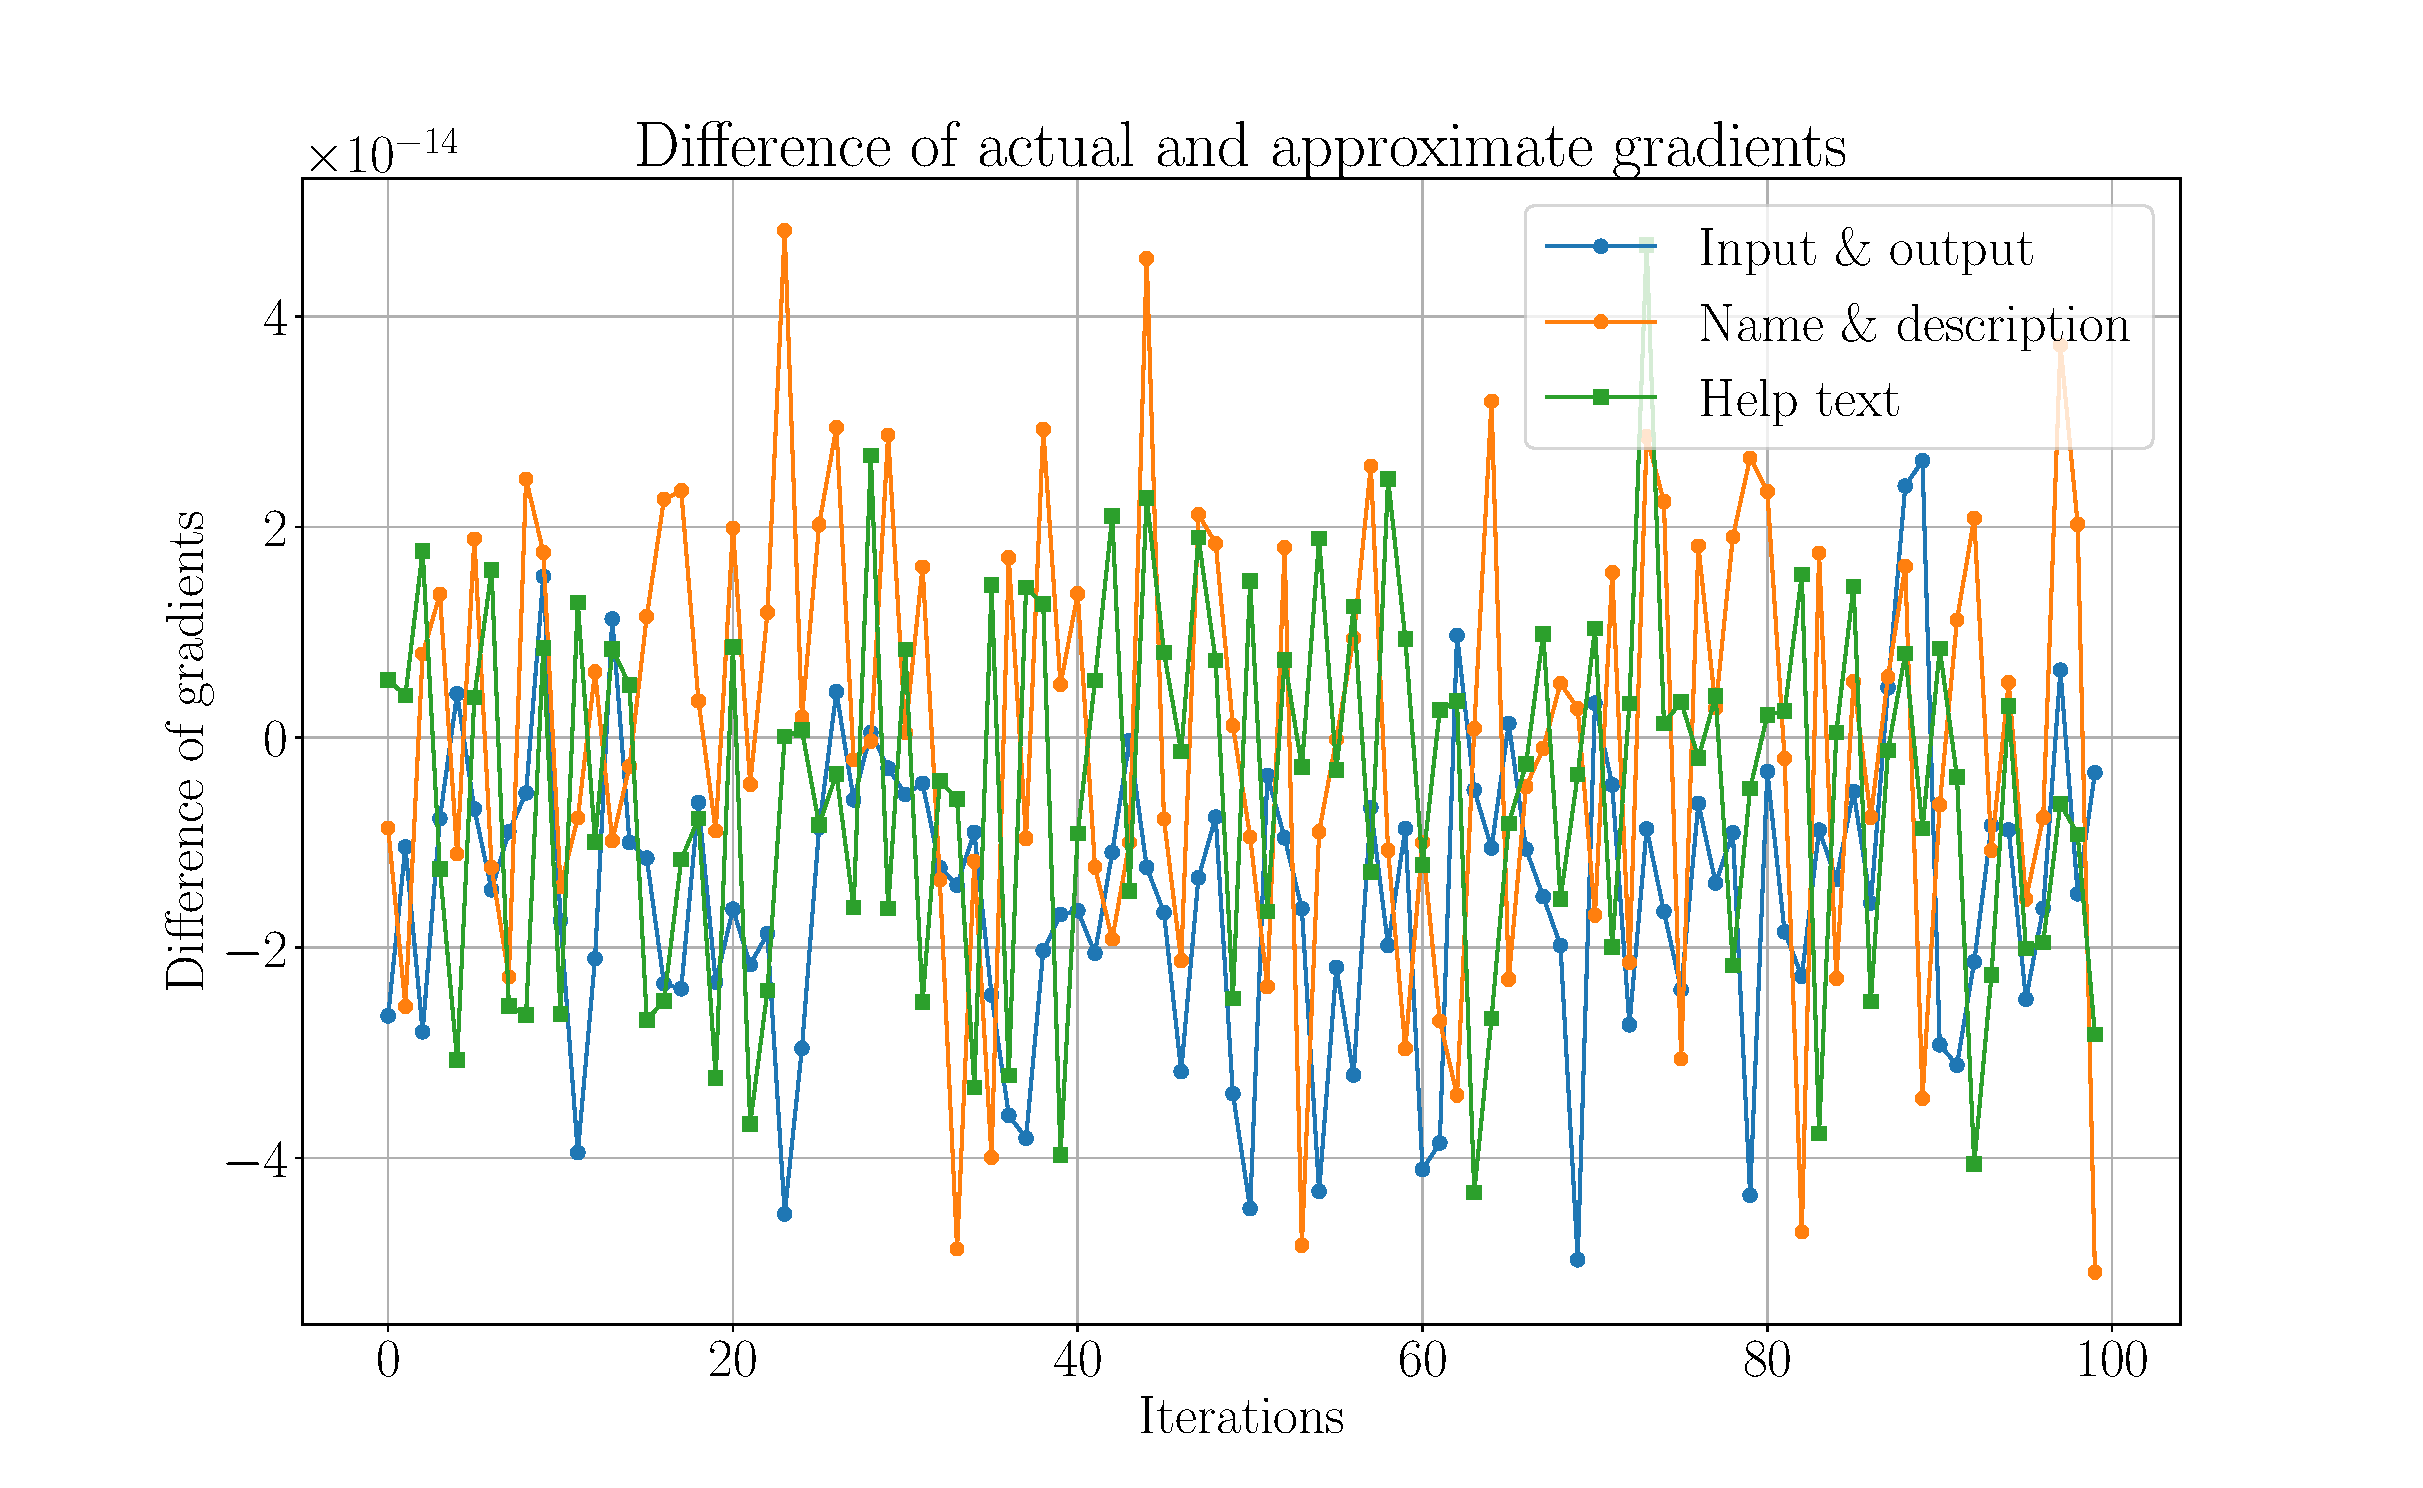
\includegraphics[scale=0.35]{figures/Difference_gradients.pdf}}
    \caption[Verification of gradient for the error function]{\textbf{Verification of gradient for the error function}: The plot checks that the difference between the actual and approximated gradients for all the attributes across all tools computed over 100 iterations is close to 0. Gradient plays an important role in learning and it should be estimated correctly. The difference of gradients is consistently $\approx 10^{-14}$ which means that the actual and approximated gradients are same and the gradient we have computed using partial derivatives is correct.}
\end{centering}
\end{figure}
    \chapter{Experiments}
\section{Amount of help text}
We take a maximum of 4 lines of text from the help text attribute while reading the xml files of tools. This attribute is noisy and contains text which is not useful to be set up as a basis for finding similarity. We need to be careful of the amount of text which we extract from this attribute. Experimentally, we verify that using $4$ lines of text from this source works better in most of the cases. The results become worse if we do not use this attribute at all.

\section{Number of attributes}
We consider three different attributes for compiling the collection of tokens. These attributes are different from each other. Using them together to make one set of tokens for each tool is not beneficial. Instead of combining the tokens from these attributes to make one set of tokens for a tool, we compute similarities using tokens from these different attributes and then combine them using an optimization technique and learn optimal weights on each attribute.

\section{Similarity measures}
For calculating similarity scores using input and output file types, we employ the jaccard index because we do not intend to learn any "concept" hidden in a set of file types for a tool. For similarities computed for name and description and help text, we use cosine similarity. Both these similarity measures give a real number between $0.0$ and $1.0$ as a similarity score for a pair of documents (tools).

\section{Latent semantic analysis}
Using latent semantic analysis, we learn dense vector representation for a document. It reduces the rank of the document-tokens matrix. We need to find out this reduction factor which can improve the similarity scores and find relevant similar tools among tools compared to using full-rank document-tokens matrix. We follow an approach of lowering the rank by certain factors and look at how the values in these matrices are spread. We reduce the rank of documents-tokens matrices to $70\%$, $30\%$ and $5\%$ of the full-rank value. Moreover, we also verify the similarity matrices corresponding to these low-rank matrices. We expect the documents-tokens and similarity matrices to be denser compared to no rank reduction. To reduce the ranks, we consider documents-tokens matrices of name and description and help text and leave the input and output matrix in its full-rank state. We use singular value decomposition method from $numpy\'s$\footnote{\url{https://docs.scipy.org/doc/numpy-1.14.0/reference/generated/numpy.linalg.svd.html}} linear algebra package.

\section{Paragraph vector}
In this approach, we learn a fixed-length dense vector for each document by setting the dimensions of these document vectors. When the size of a document is lower, we use a lower number of dimensions for the fixed-length vector. In figure 5, we see that the number of tokens is higher for help text attribute compared to the name and description attribute. To learn fixed-length vectors, we set the vector's length to be $100$ for name and description and $200$ for help text. Here as well, we learn paragraph vectors only for name and description and help text and not for input and output file types. We use $gensim\'s$ model to learn these paragraph vectors.

\subsection{Distributed bag-of-words}
Out of the two approaches to learn paragraph vectors, we apply distributed bag-of-words approach to learn vectors for each document. It does not compute word vectors and relies only on paragraph vectors to predict the randomly chosen words from a sampled text window. Learning only the paragraph vectors is faster and computationally less expensive. 

\section{Gradient descent}
To optimize the similarity scores computed from multiple attributes, we execute gradient descent optimizer to learn weights on the scores of these attributes. Based on the similarity measures, we define an error function for the optimizer which iteratively minimizes it.

\subsection{Learning rates}
We come up with a time-based decay strategy to calculate learning rate for each iteration. It starts off a higher value of $0.05$ and gradually decreases over iterations. The drop in the learning rate is smooth, neither too steep not too flat. We set a maximum iteration of 100 within which the learning saturates comfortably. When we start with $0.1$ or higher, there is a risk of optimizer divergence. If we start with $0.001$, the learning does not saturate within $100$ iterations (the learning becomes slow). 

\section{Code repositories}
The codebase used for this study is at github. There are separate branches for the different ideas discussed here. For latent semantic analysis approach, we have two branches - one uses full-rank documents-tokens matrices\footnote{\url{https://github.com/anuprulez/similar_galaxy_tools/tree/lsi}} and another uses documents-tokens matrices reduced to $5\%$ of the full-rank\footnote{\url{https://github.com/anuprulez/similar_galaxy_tools/tree/lsi_005}}. Both these branches differ only in their ranks of documents-tokens matrices. There is a separate branch for paragraph vectors approach\footnote{\url{https://github.com/anuprulez/similar_galaxy_tools/tree/doc2vec}}. All these code repositories are under MIT License\footnote{\url{https://github.com/anuprulez/similar_galaxy_tools/blob/master/LICENSE.md}}.
    \chapter{Results and Analysis}
% screenshots of the results - positive and negative
\section{Latent Semantic Analysis}
We experiment with multiple values of matrix rank reduction and we find that as we reduce the rank of documents-tokens matrices, they become more dense. As we reduce the ranks, the distribution of  the learnt weights also change. 

\subsection{Full-rank matrices}
Figure 17 shows the similarity matrices computed using full-rank documents-tokens matrices for input and output (17a), name and description (17b) and help text (17c) attributes. We do not apply rank reduction on documents-tokens matrix of input and output file types. Using these similarity matrices, we learn each row's respective importance factor using gradient descent and then combine to get a weighted average similarity matrix (17d). Figure 18 shows the distribution of these importance factors (weights) for multiple tool attributes and we see that the magnitude of weights estimated for input and output file types is higher than the other two attributes. The high magnitude is associated with the higher values captured for the similarity matrix of input and output file types (17a). 

\begin{figure}[h]
\begin{centering}
    {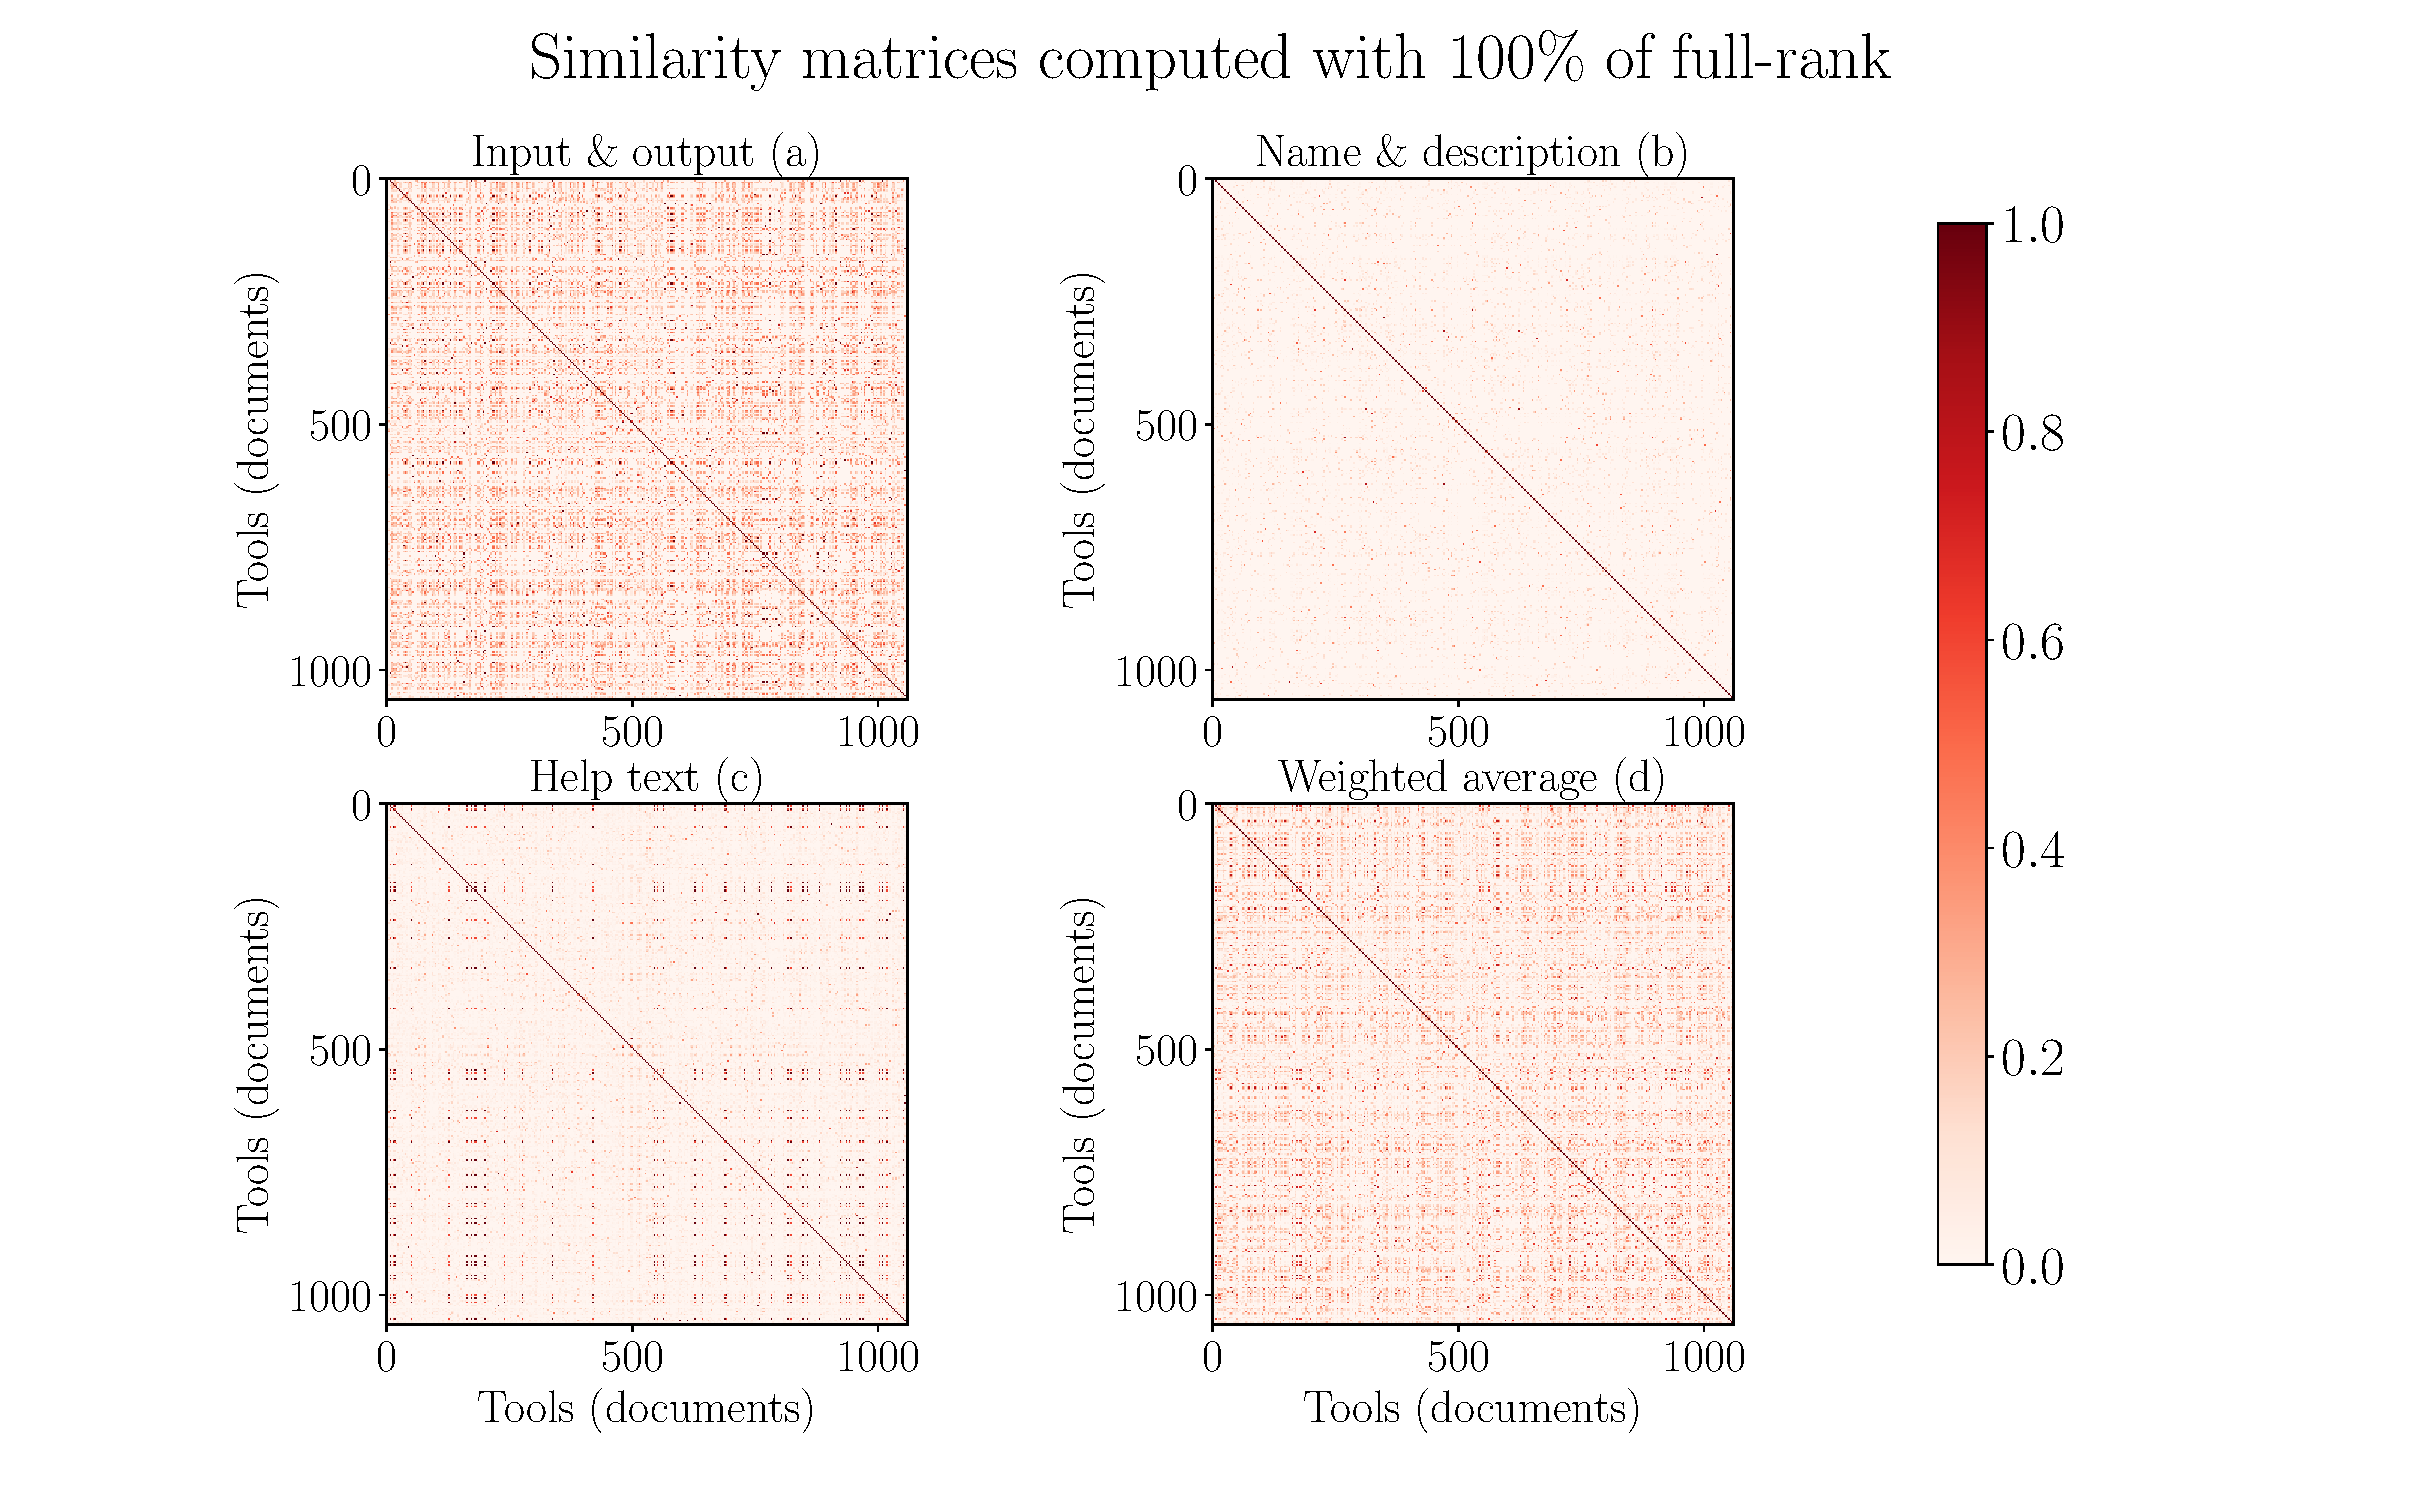
\includegraphics[scale=0.35]{figures/Similarity_matrices_100.pdf}}
    \caption[Similarity matrices full rank]{\textbf{Similarity matrices using full-rank}: The heatmap shows documents-documents (tools-tools) correlation matrices for input and output (a), name and description (b) and help text (c) attributes. The (d) shows a documents-documents (tools-tools) correlation matrix which is the weighted average computed using (a), (b) and (c) and weights (figure 18) given by the gradient descent optimizer (equation 15). The corresponding documents-tokens matrices contain their full-ranks. }
\end{centering}
\end{figure}

\begin{figure}[h]
\begin{centering}
    {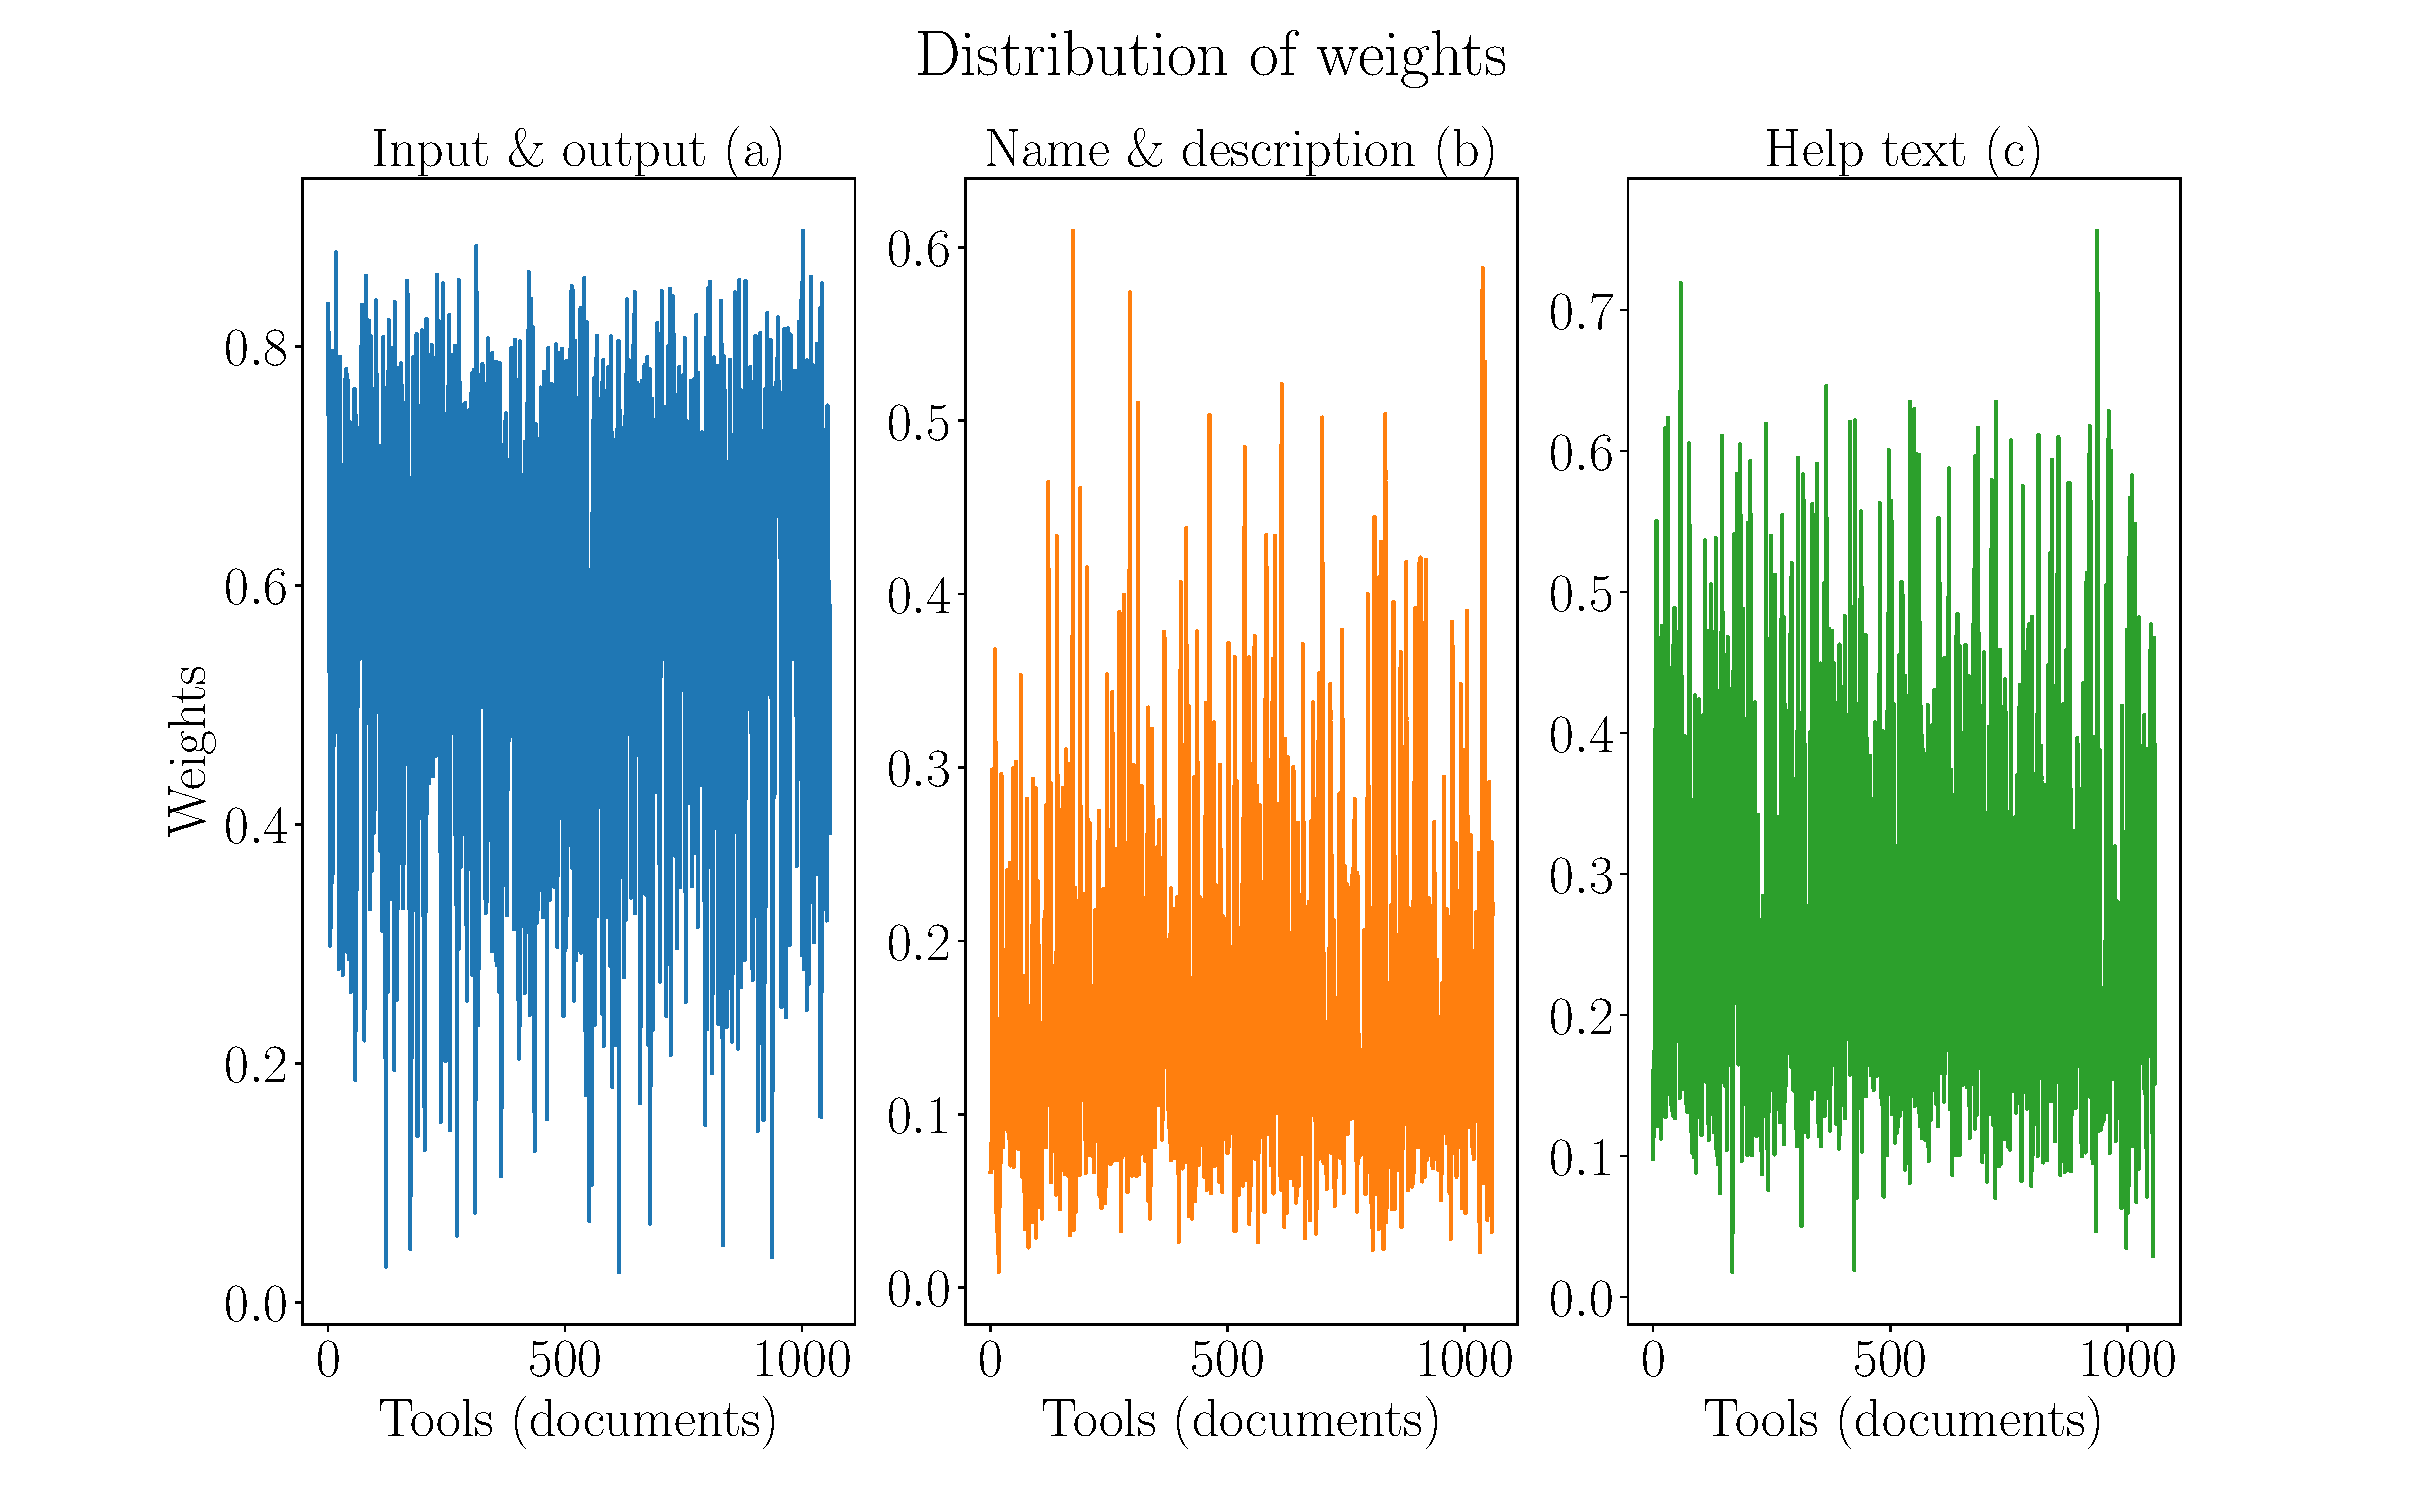
\includegraphics[scale=0.35]{figures/Weights_100.pdf}}
    \caption[Weights distribution full-rank]{\textbf{Weights distribution full- rank}: The plot shows the distribution of weights learned by gradient descent optimizer on the similarity matrices for the input and output, name and description and help text attributes. The corresponding documents-tokens matrices contain their full-ranks.}
\end{centering}
\end{figure}

\subsection{70\% of full-rank}
In figure 17, we can see that the similarity matrices for name and description and help text are sparse. To reduce the sparsity,  we attempt to reduce the ranks of the respective documents-tokens matrices of these two attributes to 70\% of full-rank. For example, if the rank of a matrix is 100, we reduce the rank to 70 using singular value decomposition. Along with reducing the ranks, we reduce the singular values of these matrices as well. Comparing figures 17 and 19, we see that the name and description and help text similarity matrices start becoming more dense. The distribution of the weights also change (figures 18 and 20). At this stage, it is hard to see the effect of rank reduction. Further we reduce the ranks drastically to see the effect.

\begin{figure}[h]
\begin{centering}
    {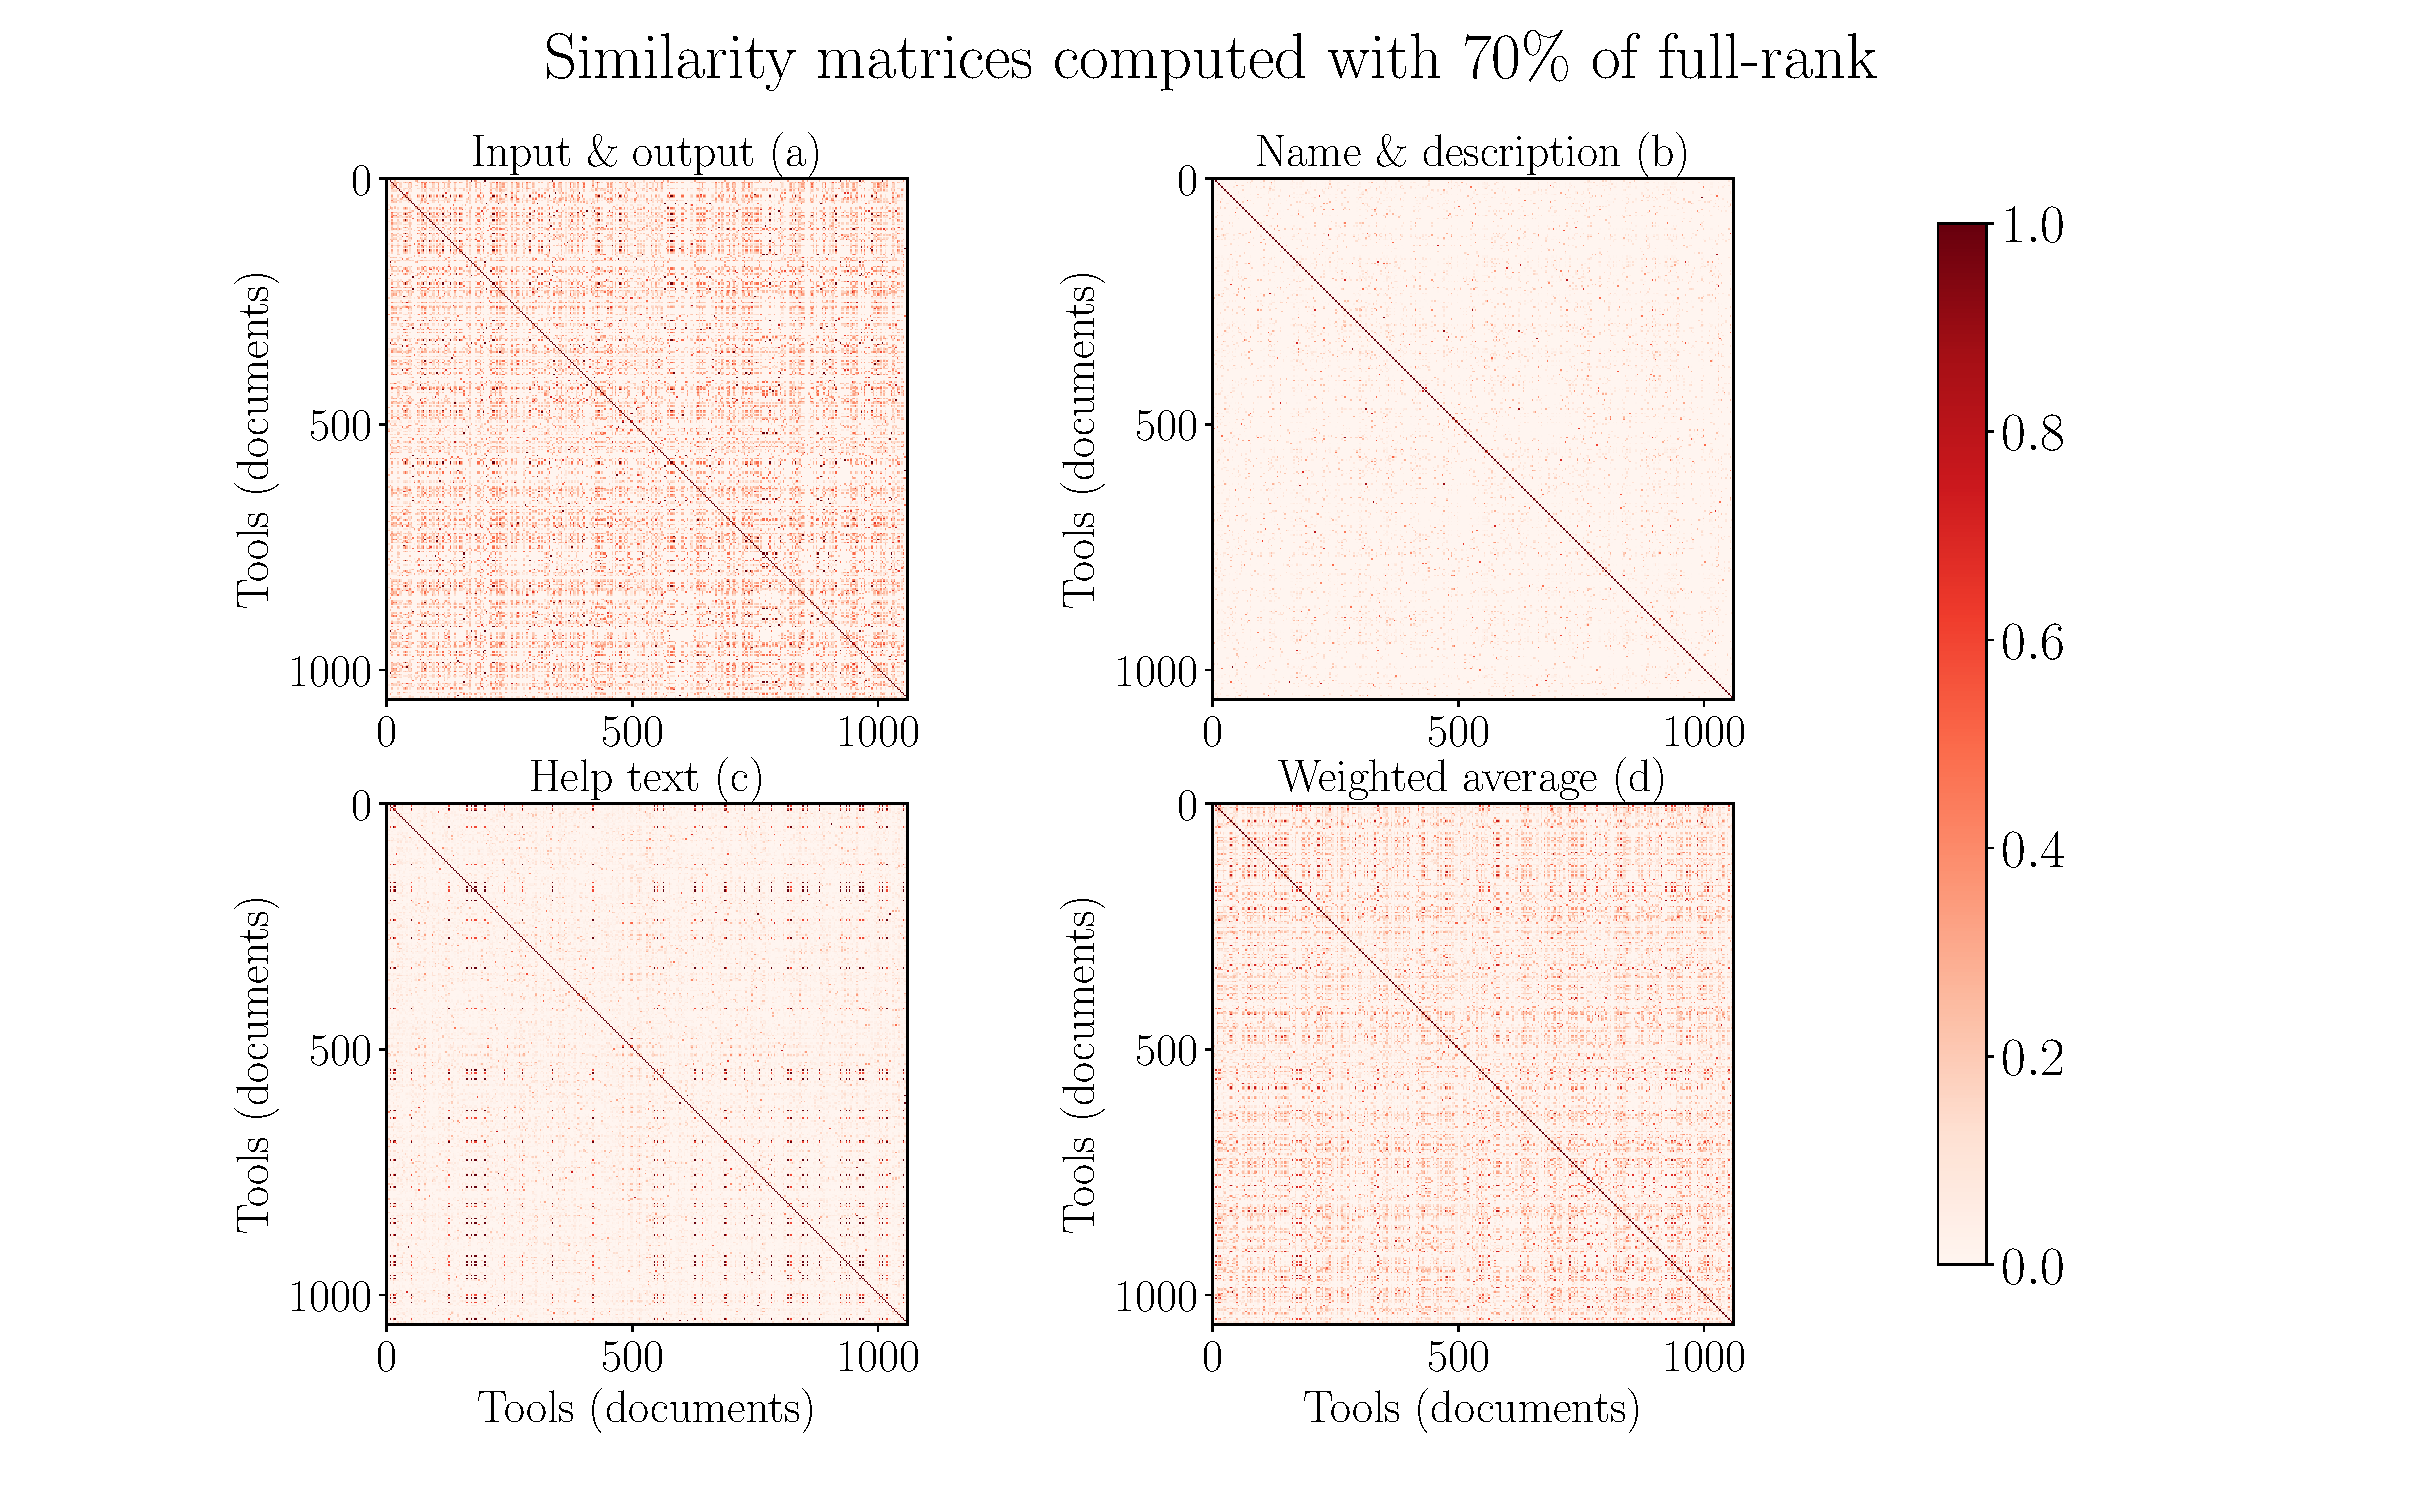
\includegraphics[scale=0.35]{figures/Similarity_matrices_070.pdf}}
    \caption[Similarity matrices 70\% rank]{\textbf{Similarity matrices using 70\% of full-rank}: The heatmap shows documents-documents (tools-tools) correlation matrices for input and output (a), name and description (b) and help text (c) attributes. The (d) shows a documents-documents (tools-tools) correlation matrix which is the weighted average computed using (a), (b) and (c) and weights (figure 20) given by the gradient descent optimizer (equation 15). The corresponding documents-tokens matrices are reduced to 70\% of their respective full-ranks.}
\end{centering}
\end{figure}

\begin{figure}[h]
\begin{centering}
    {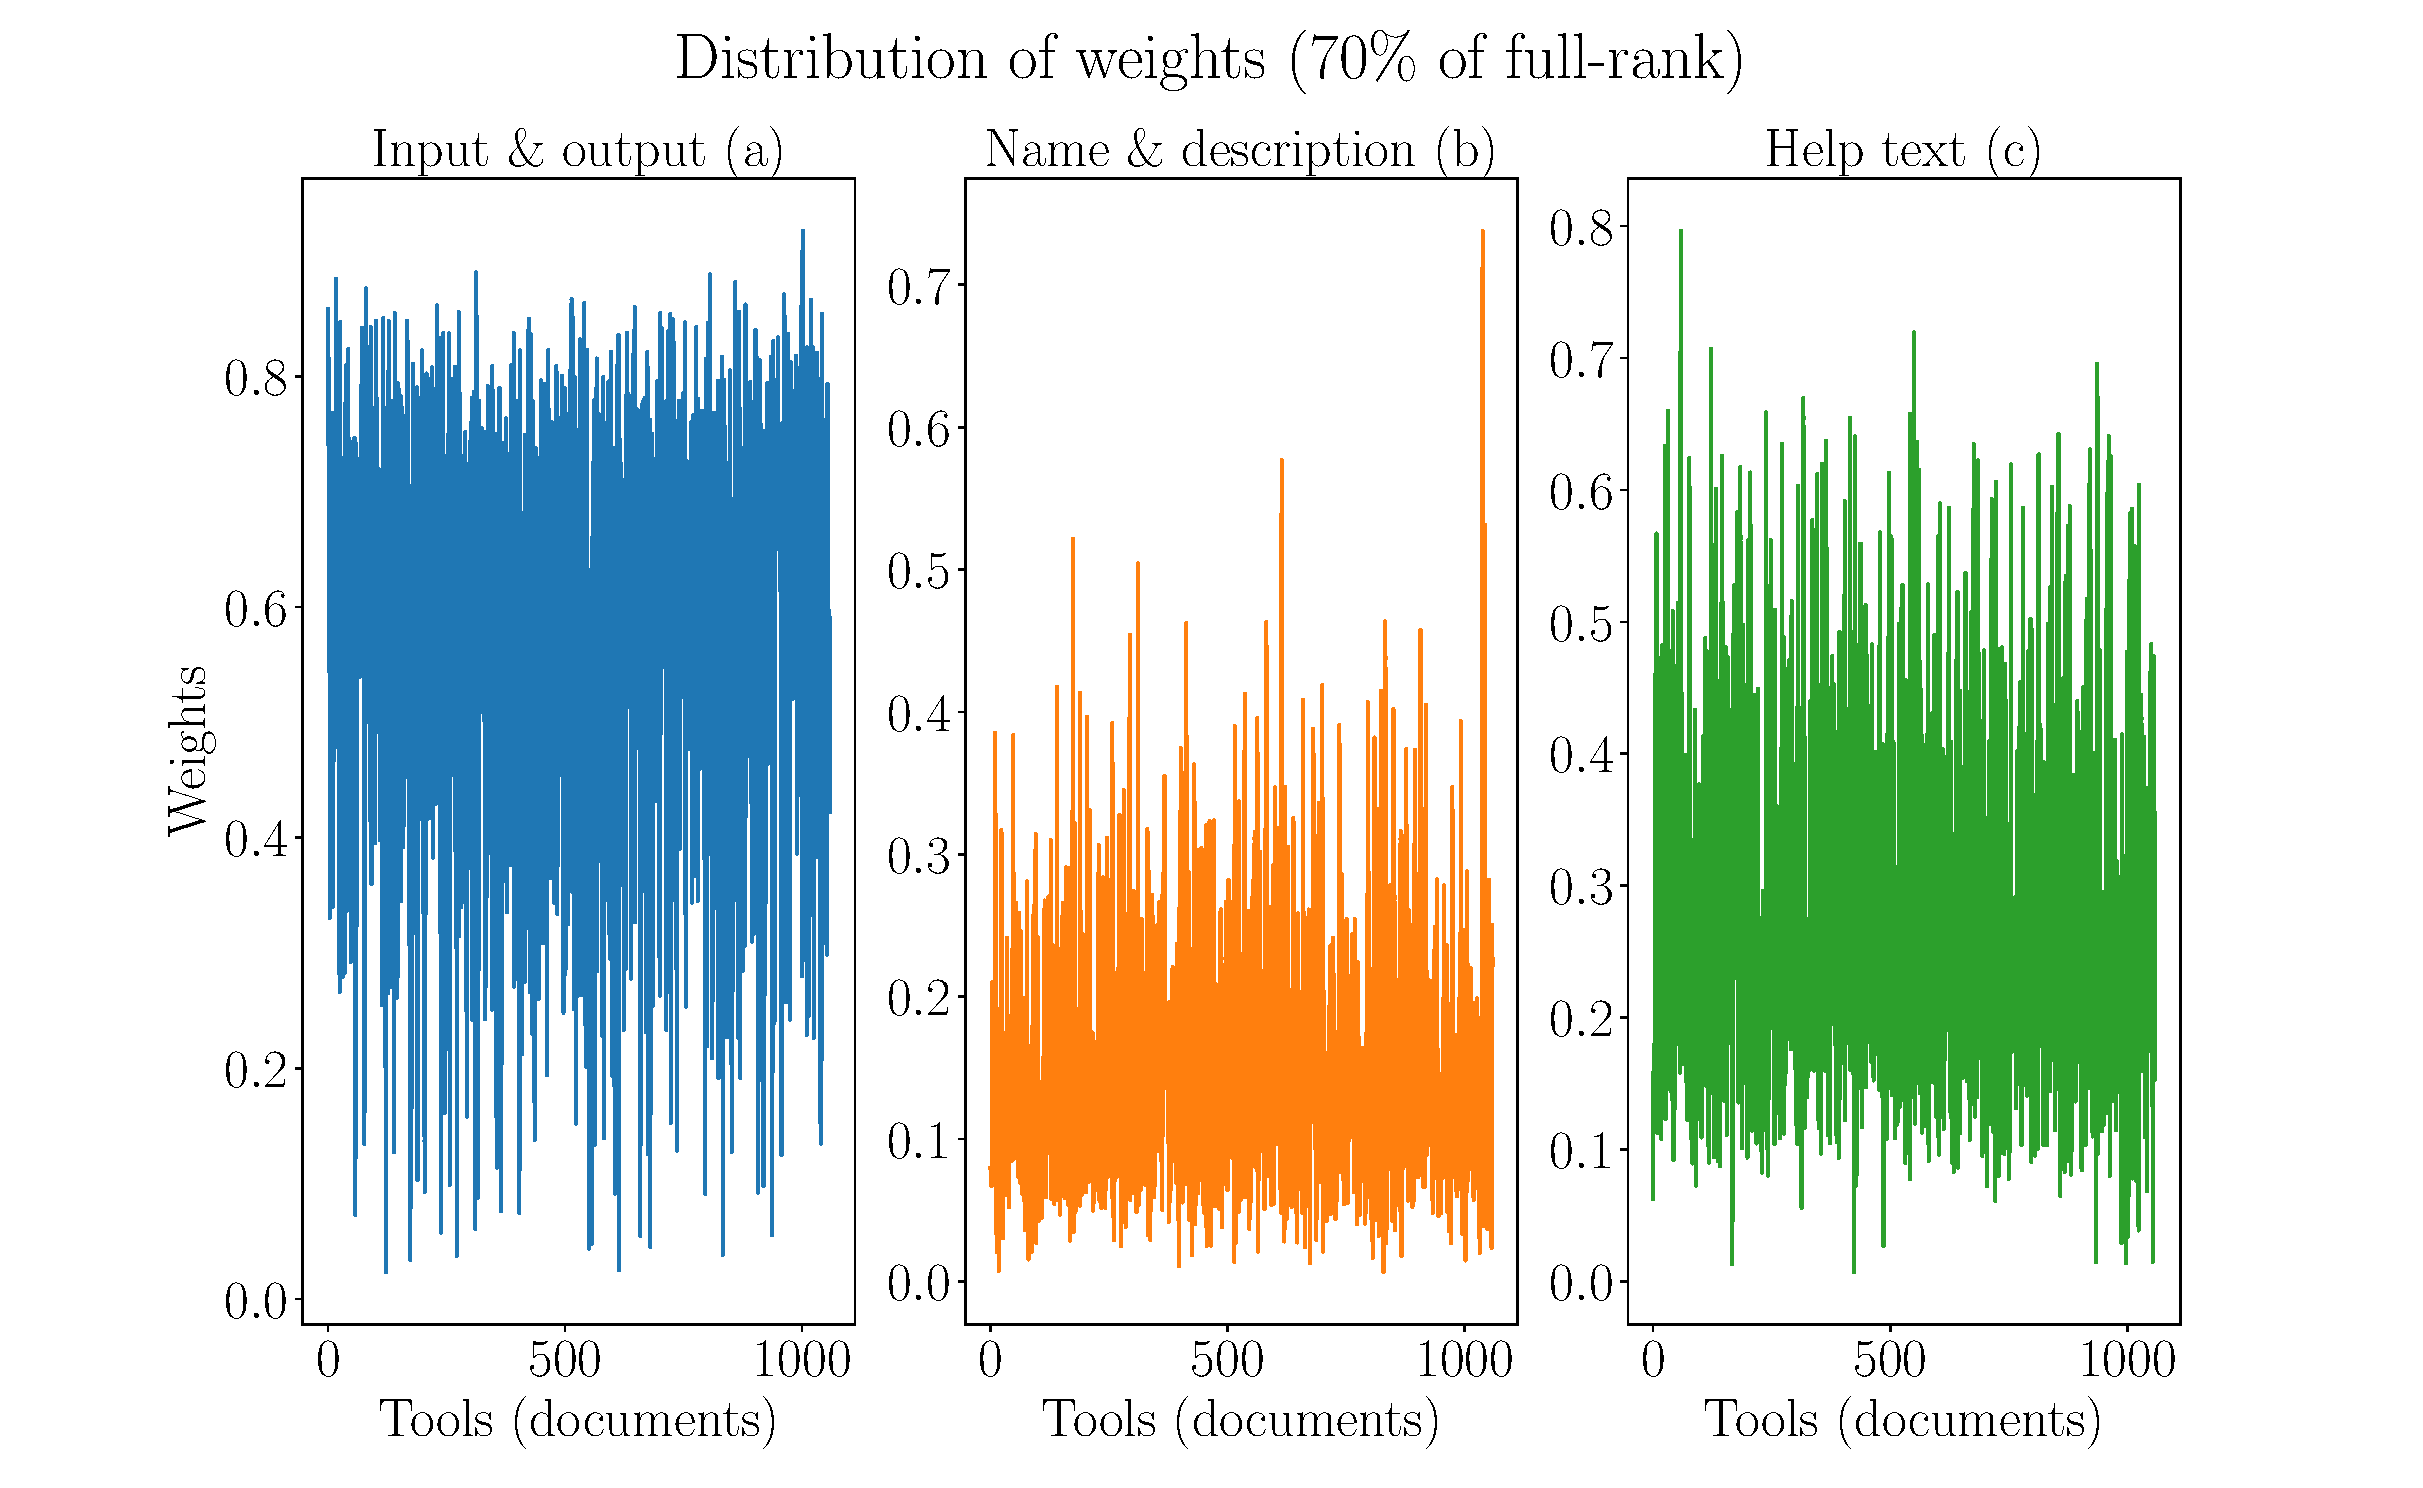
\includegraphics[scale=0.35]{figures/Weights_070.pdf}}
    \caption[Weights distribution 70\% rank]{\textbf{Weights distribution using 70\% of full-rank}: The plot shows the distribution of weights learned by gradient descent optimizer on the similarity matrices for the input and output, name and description and help text attributes. The corresponding documents-tokens matrices contain 70\% of their full-ranks.}
\end{centering}
\end{figure}

\subsection{30\% of full-rank}
To see the effect of rank reduction, we reduce the ranks of two documents-tokens matrices to 30\% of full-rank. This is a large reduction and would amount to keeping $\approx 60\%$ (removing $\approx 40\%$) (figure 11) of sum of singular values for all the documents-tokens matrices. In figures 21 and 22, the effect of rank reduction is more visible compared to $70\%$. We see that the magnitudes of weights learned for input and output files start to decrease and the magnitudes of weights for name and description and help text start to increase because the corresponding similarity matrices score become more dense (figure 21). 

\begin{figure}[h]
\begin{centering}
    {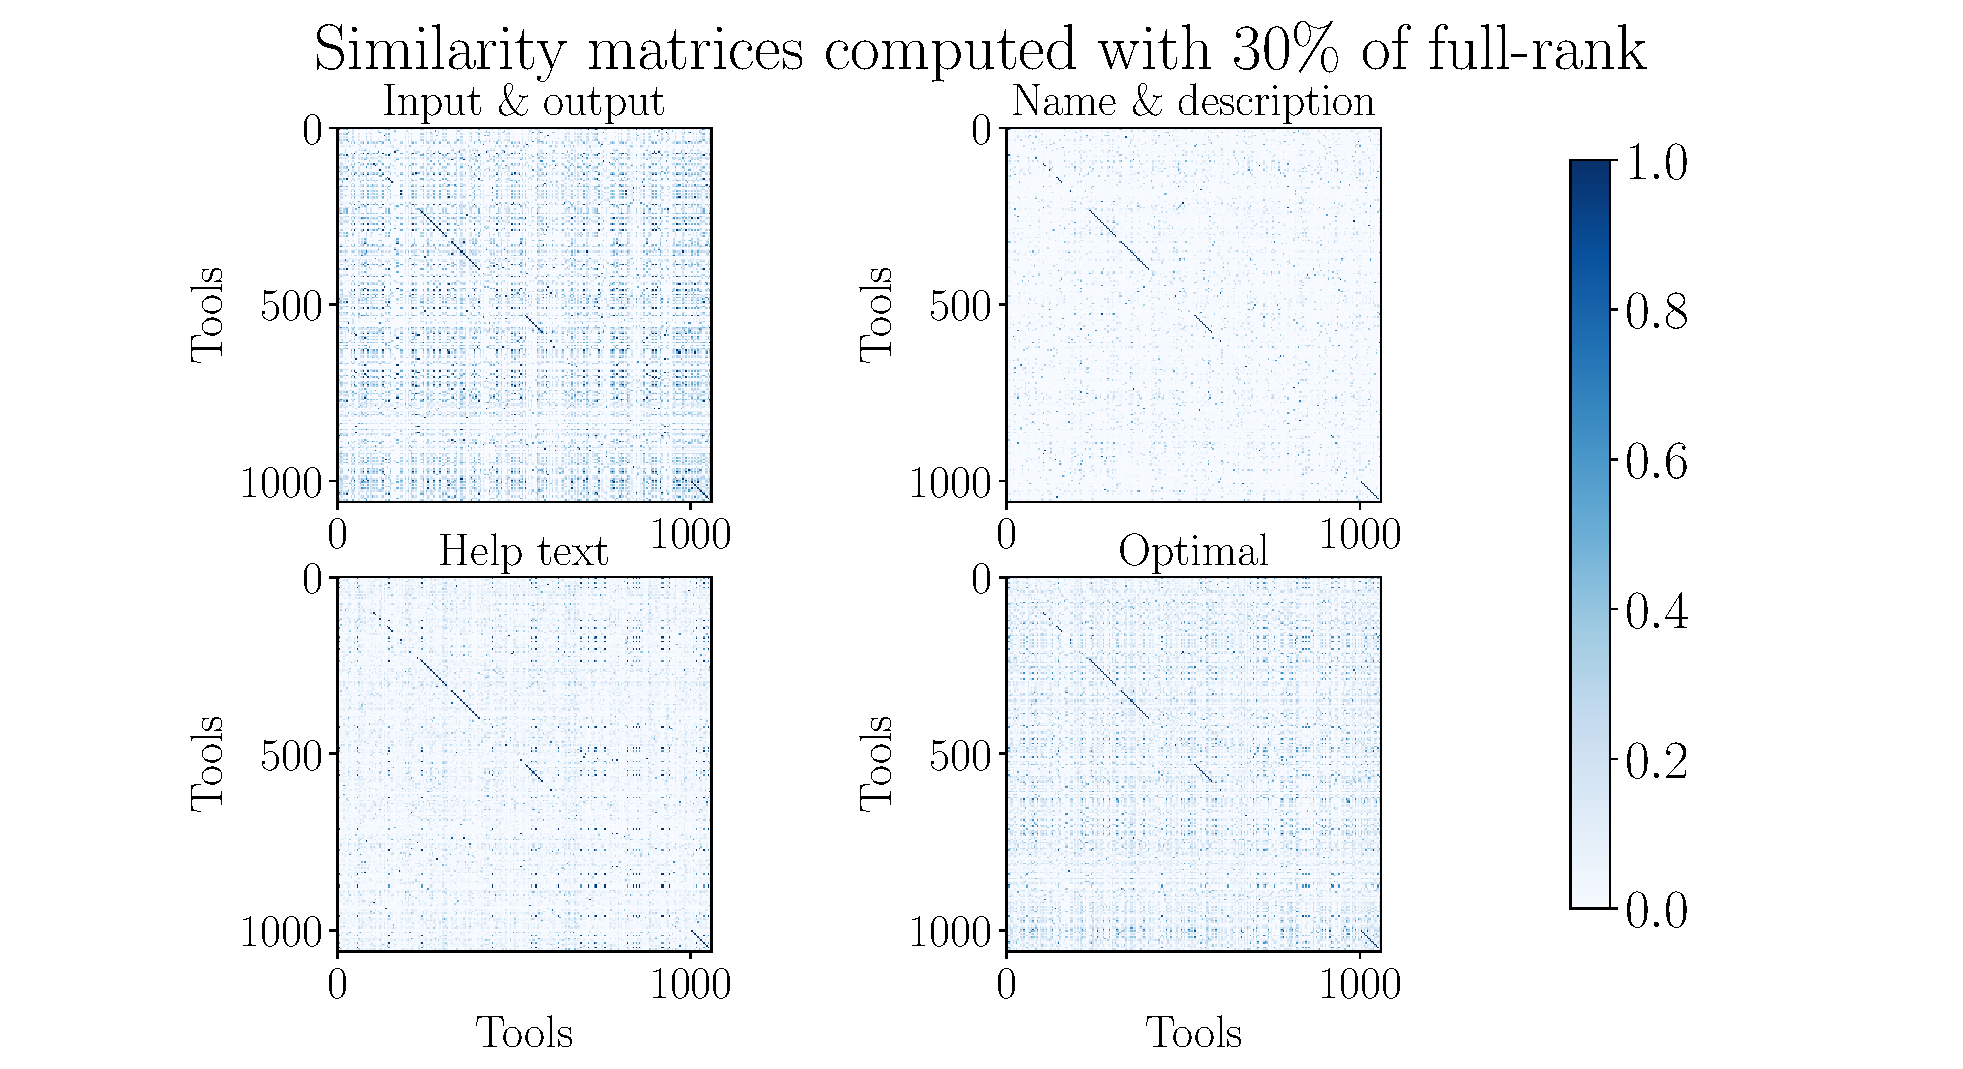
\includegraphics[scale=0.35]{figures/Similarity_matrices_030.pdf}}
    \caption[Similarity matrices 30\% rank]{\textbf{Similarity matrices using 30\% of full-rank}: The heatmap shows documents-documents (tools-tools) correlation matrices for input and output (a), name and description (b) and help text (c) attributes. The (d) shows a documents-documents (tools-tools) correlation matrix which is the weighted average computed using (a), (b) and (c) and weights (figure 22) given by the gradient descent optimizer (equation 15). The corresponding documents-tokens matrices are reduced to 30\% of their respective full-ranks.}
\end{centering}
\end{figure}

\begin{figure}[h]
\begin{centering}
    {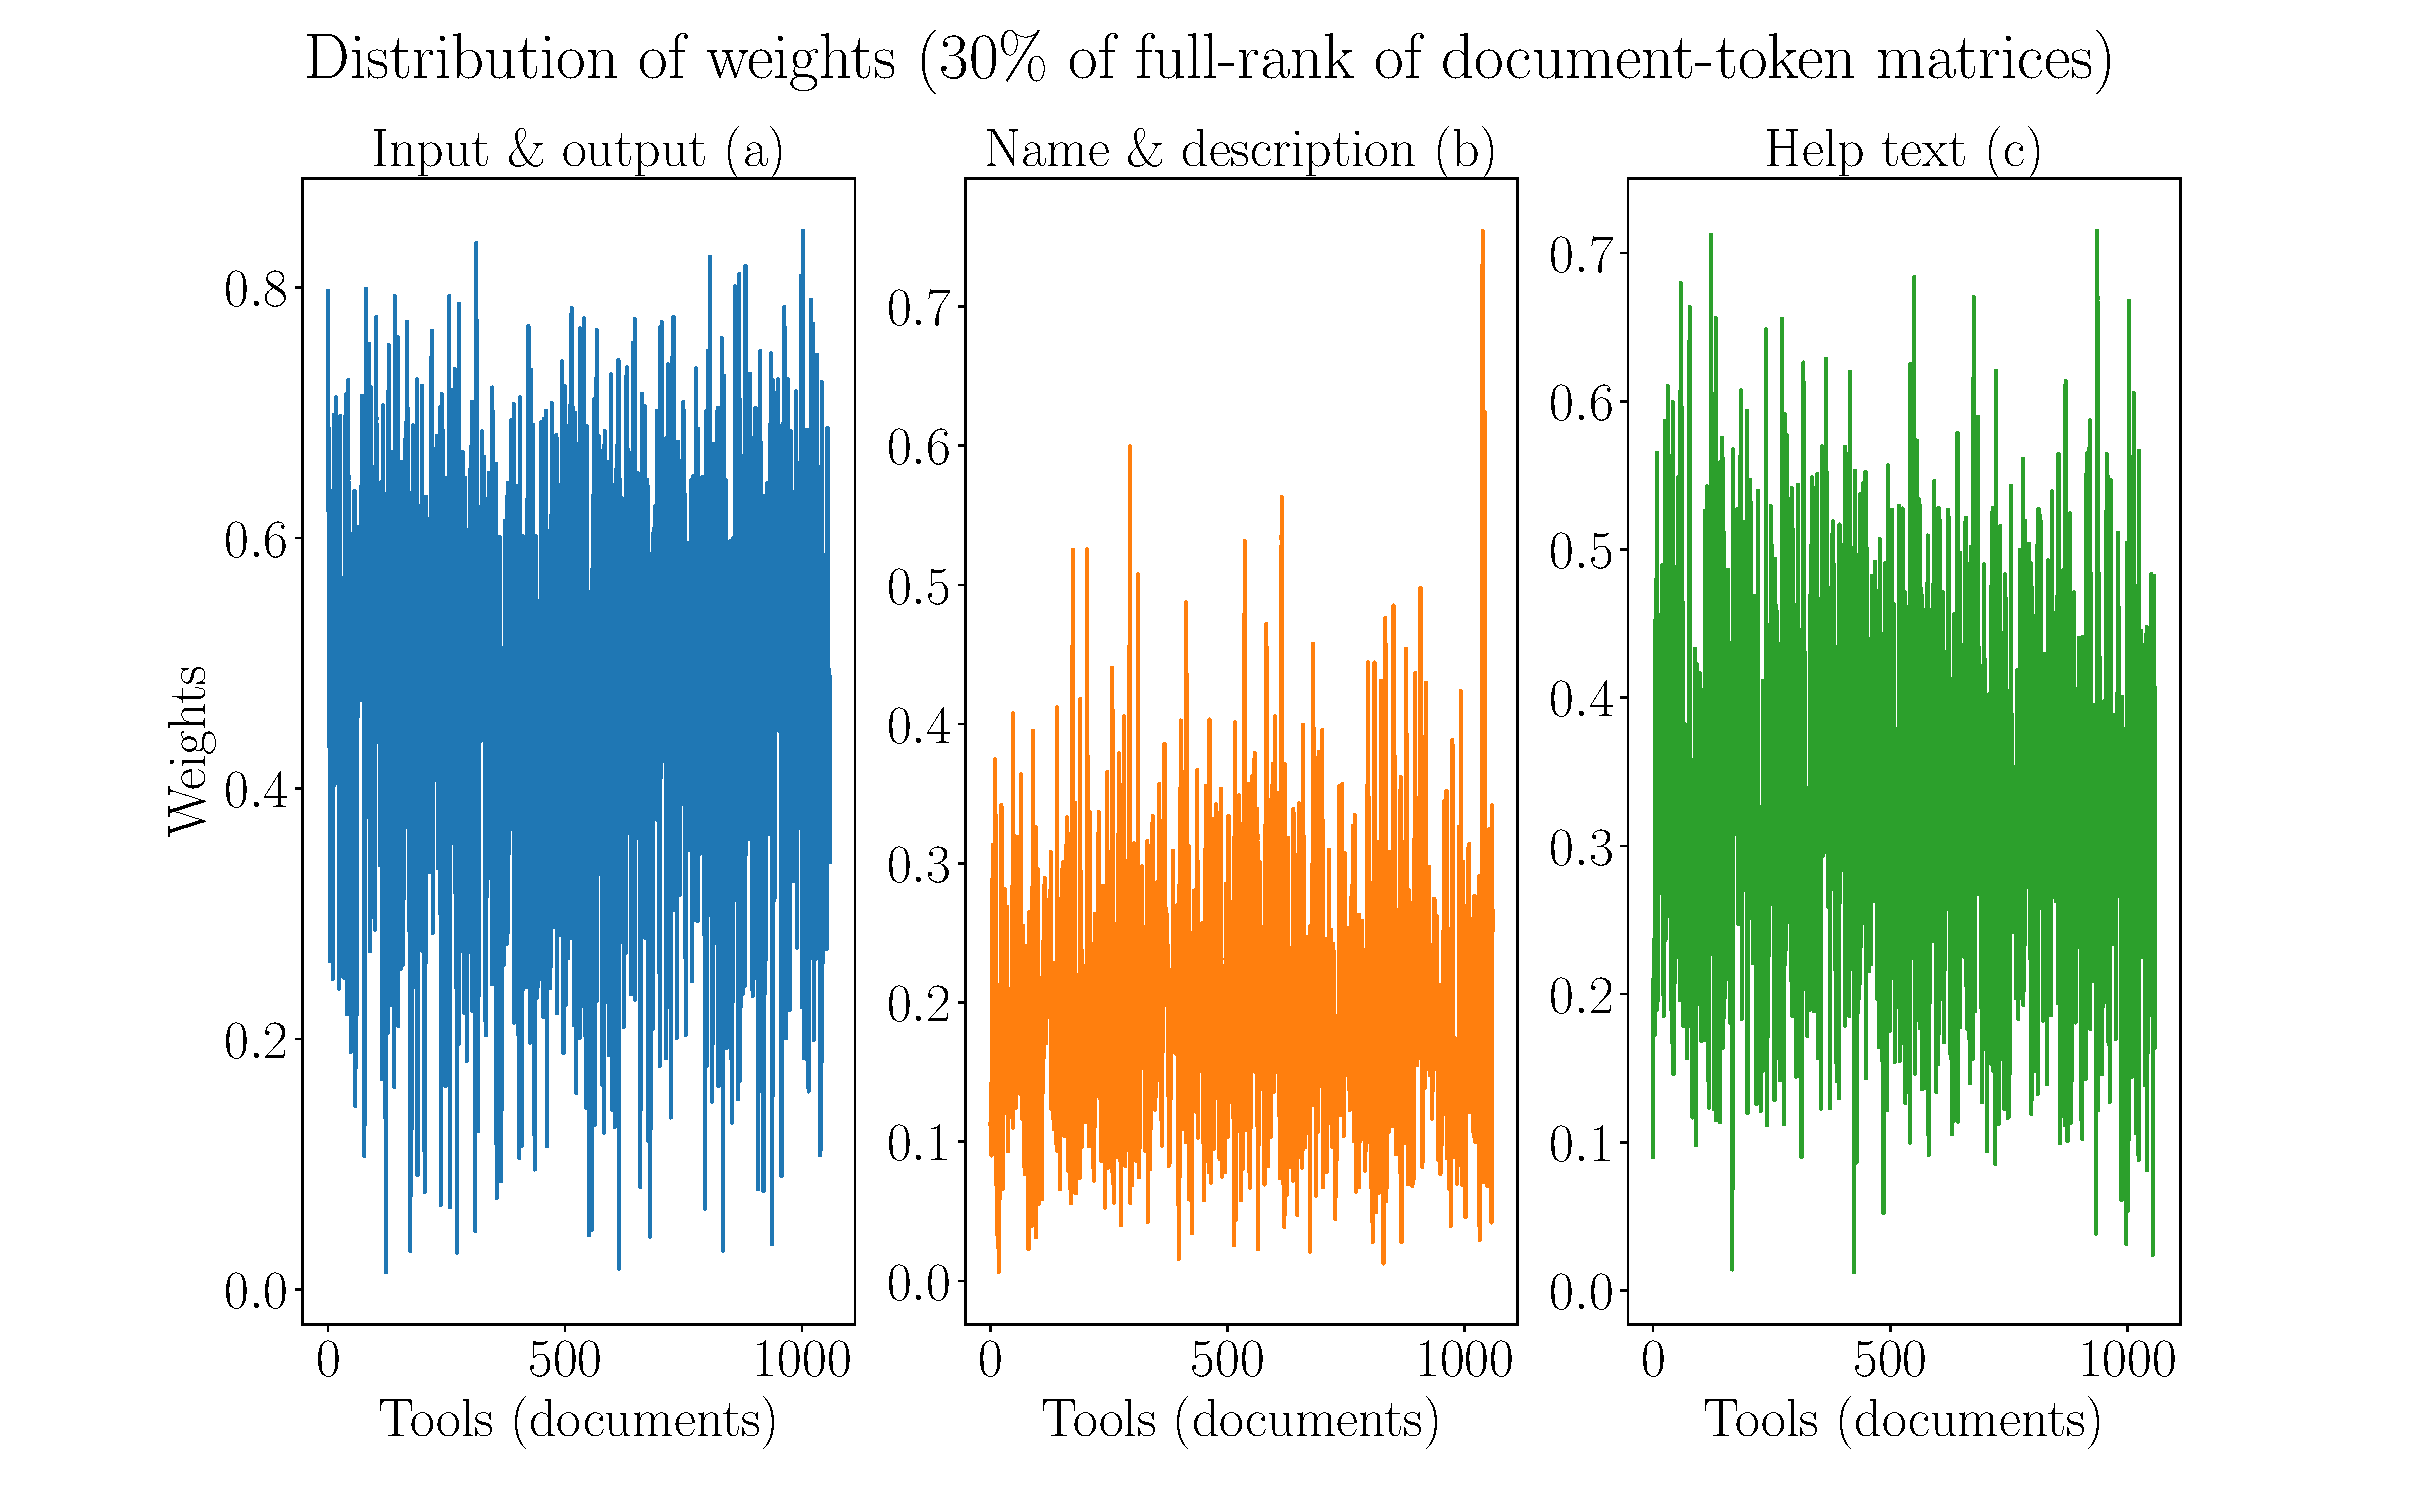
\includegraphics[scale=0.35]{figures/Weights_030.pdf}}
    \caption[Weights distribution 30\% rank]{\textbf{Weights distribution using 30\% of full-rank}: The plot shows the distribution of weights learned by gradient descent optimizer on the similarity matrices for the input and output, name and description and help text attributes. The corresponding documents-tokens matrices contain 30\% of their full-ranks.}
\end{centering}
\end{figure}

\subsection{5\% of full-rank}
To verify the reduction in sparsity, we reduce the ranks of two documents-tokens matrices to 5\% of the full-rank. By choosing this low value, we consider only top $\approx 20\%$ of the sum of singular values for all the attributes (figure 11). From figure 23, we can see that all the similarity matrices corresponding to the attributes become more dense compared to figure 17, 91 and 21. Due to this, the weights distribution also change (figure 24). We learn higher weights for name and description (24b) and help text (24c). Along side, the weights on the input and output file types decrease (24a).  

\begin{figure}[h]
\begin{centering}
    {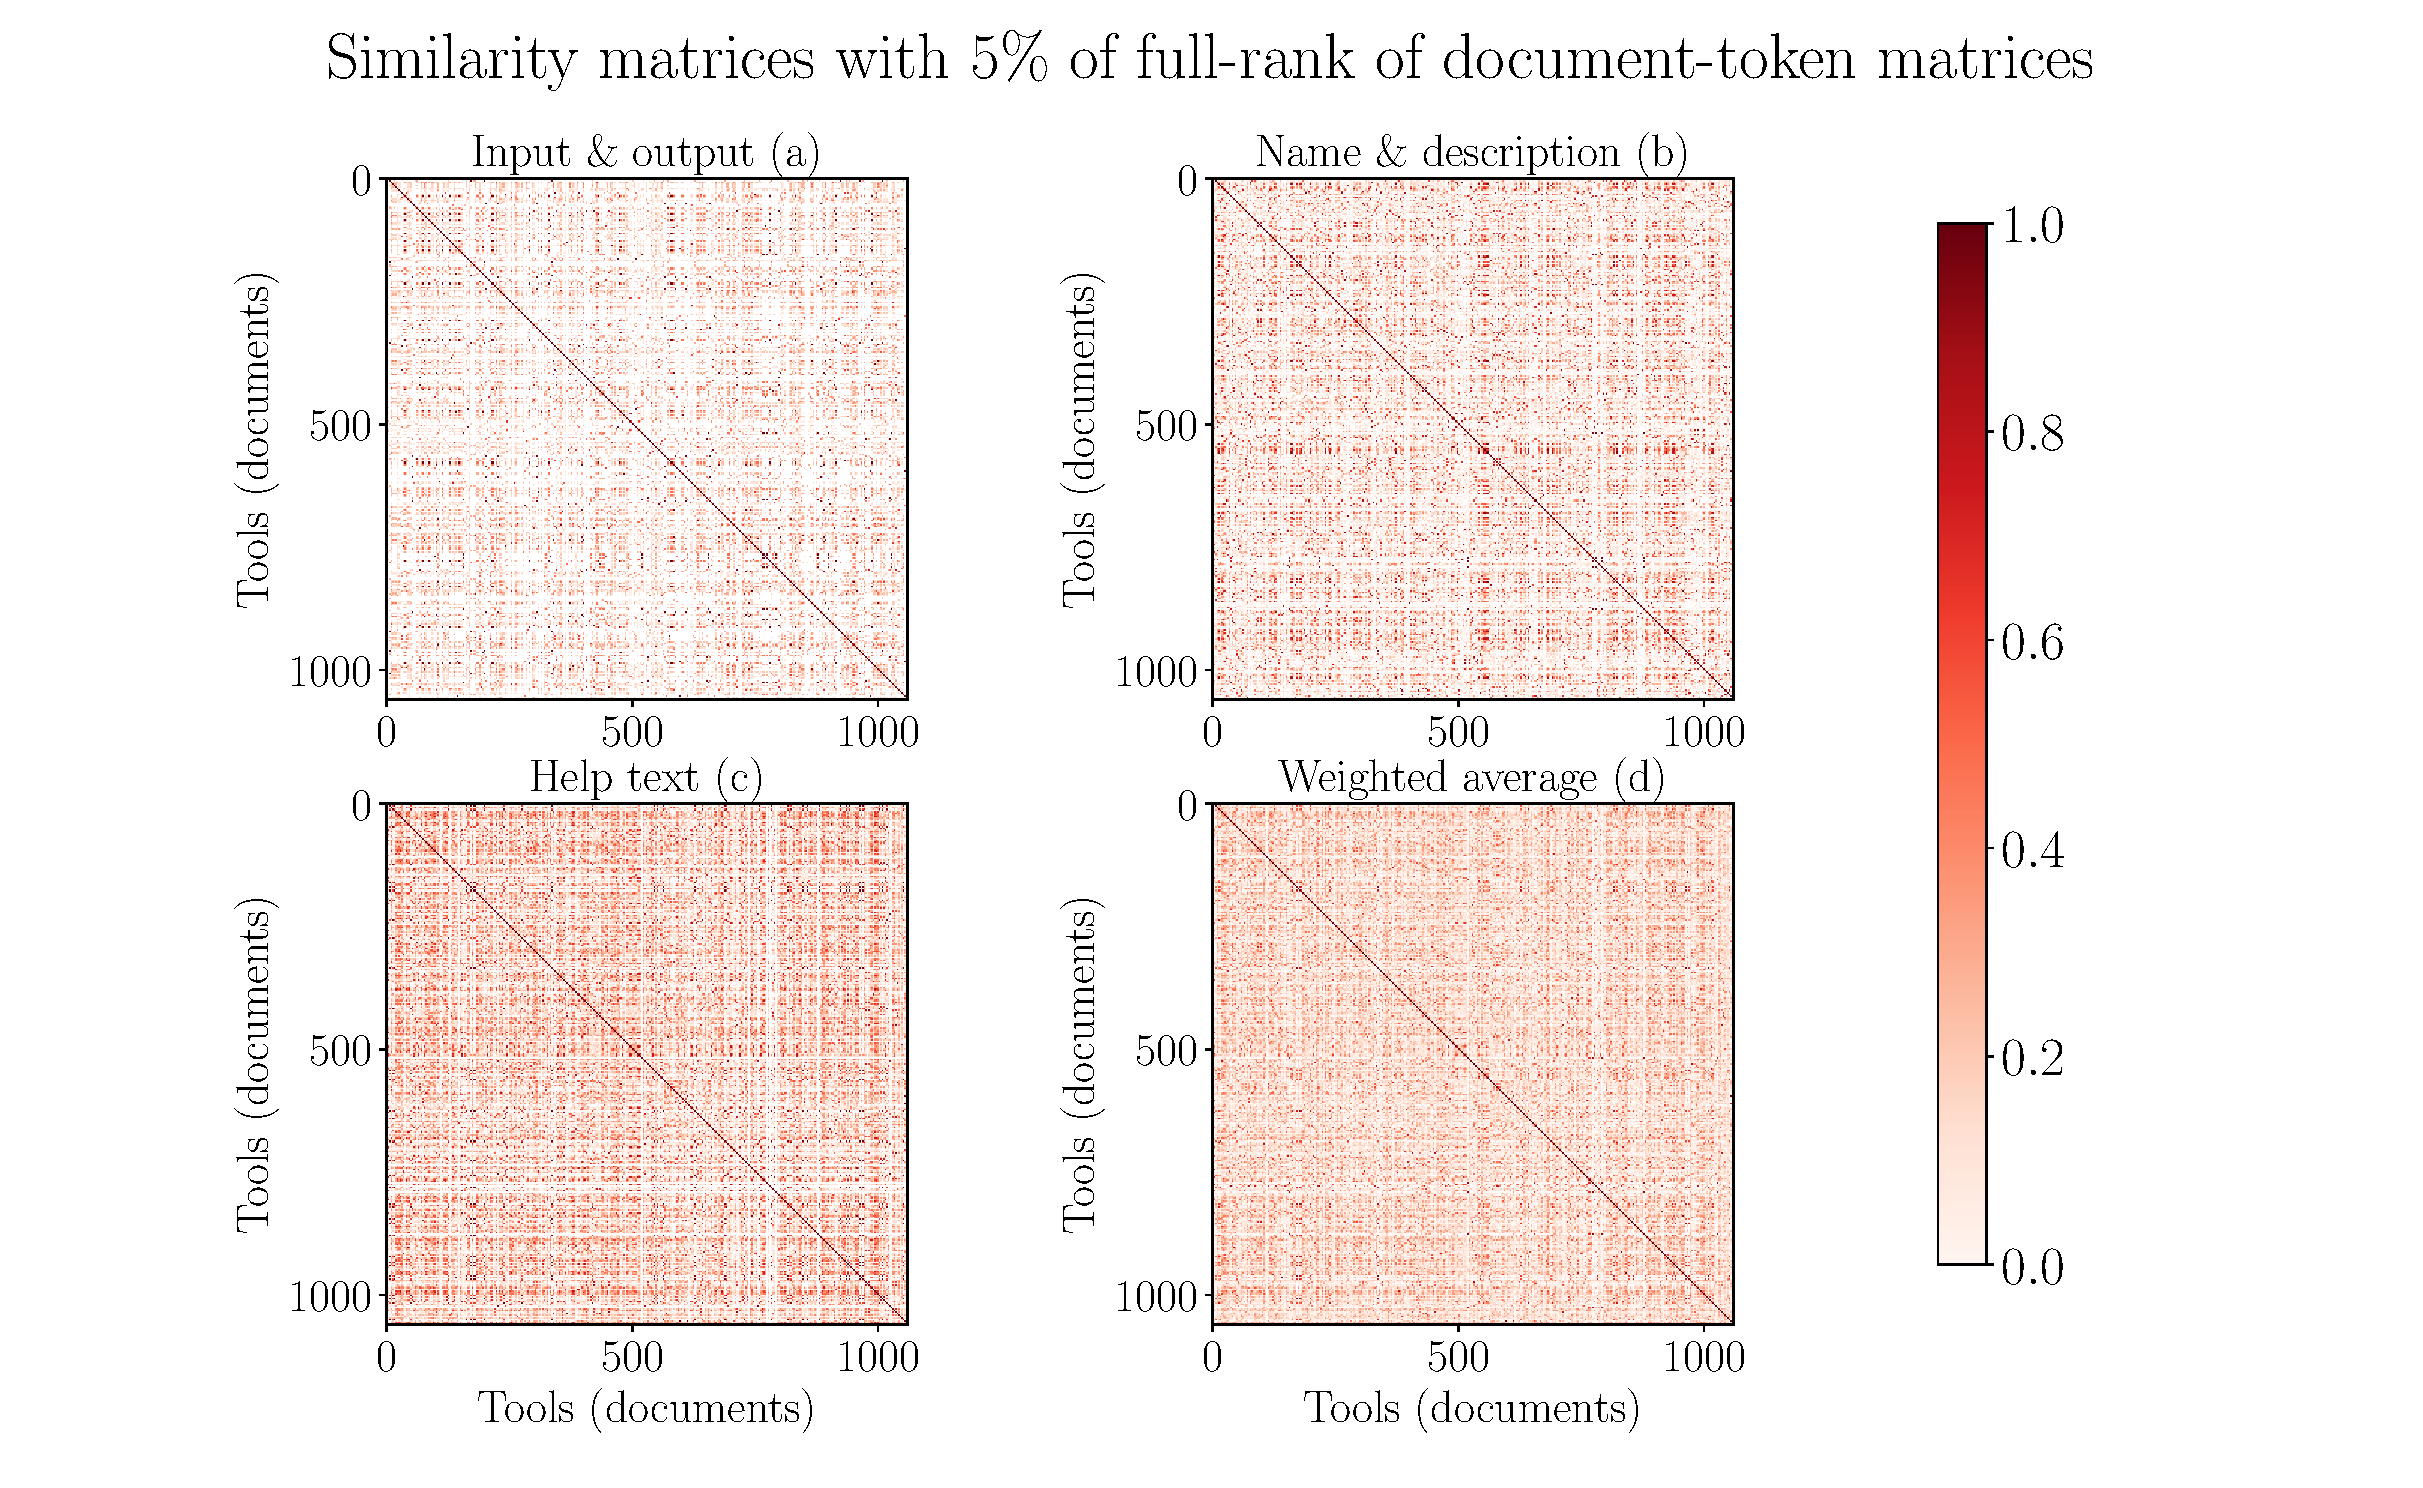
\includegraphics[scale=0.35]{figures/Similarity_matrices_005.pdf}}
    \caption[Similarity matrices 5\% rank]{\textbf{Similarity matrices using 5\% of full-rank}: The heatmap shows documents-documents (tools-tools) correlation matrices for input and output (a), name and description (b) and help text (c) attributes. The (d) shows a documents-documents (tools-tools) correlation matrix which is the weighted average computed using (a), (b) and (c) and weights (figure 24) given by the gradient descent optimizer (equation 15). The corresponding documents-tokens matrices are reduced to 5\% of their respective full-ranks.}
\end{centering}
\end{figure}

\begin{figure}[h]
\begin{centering}
    {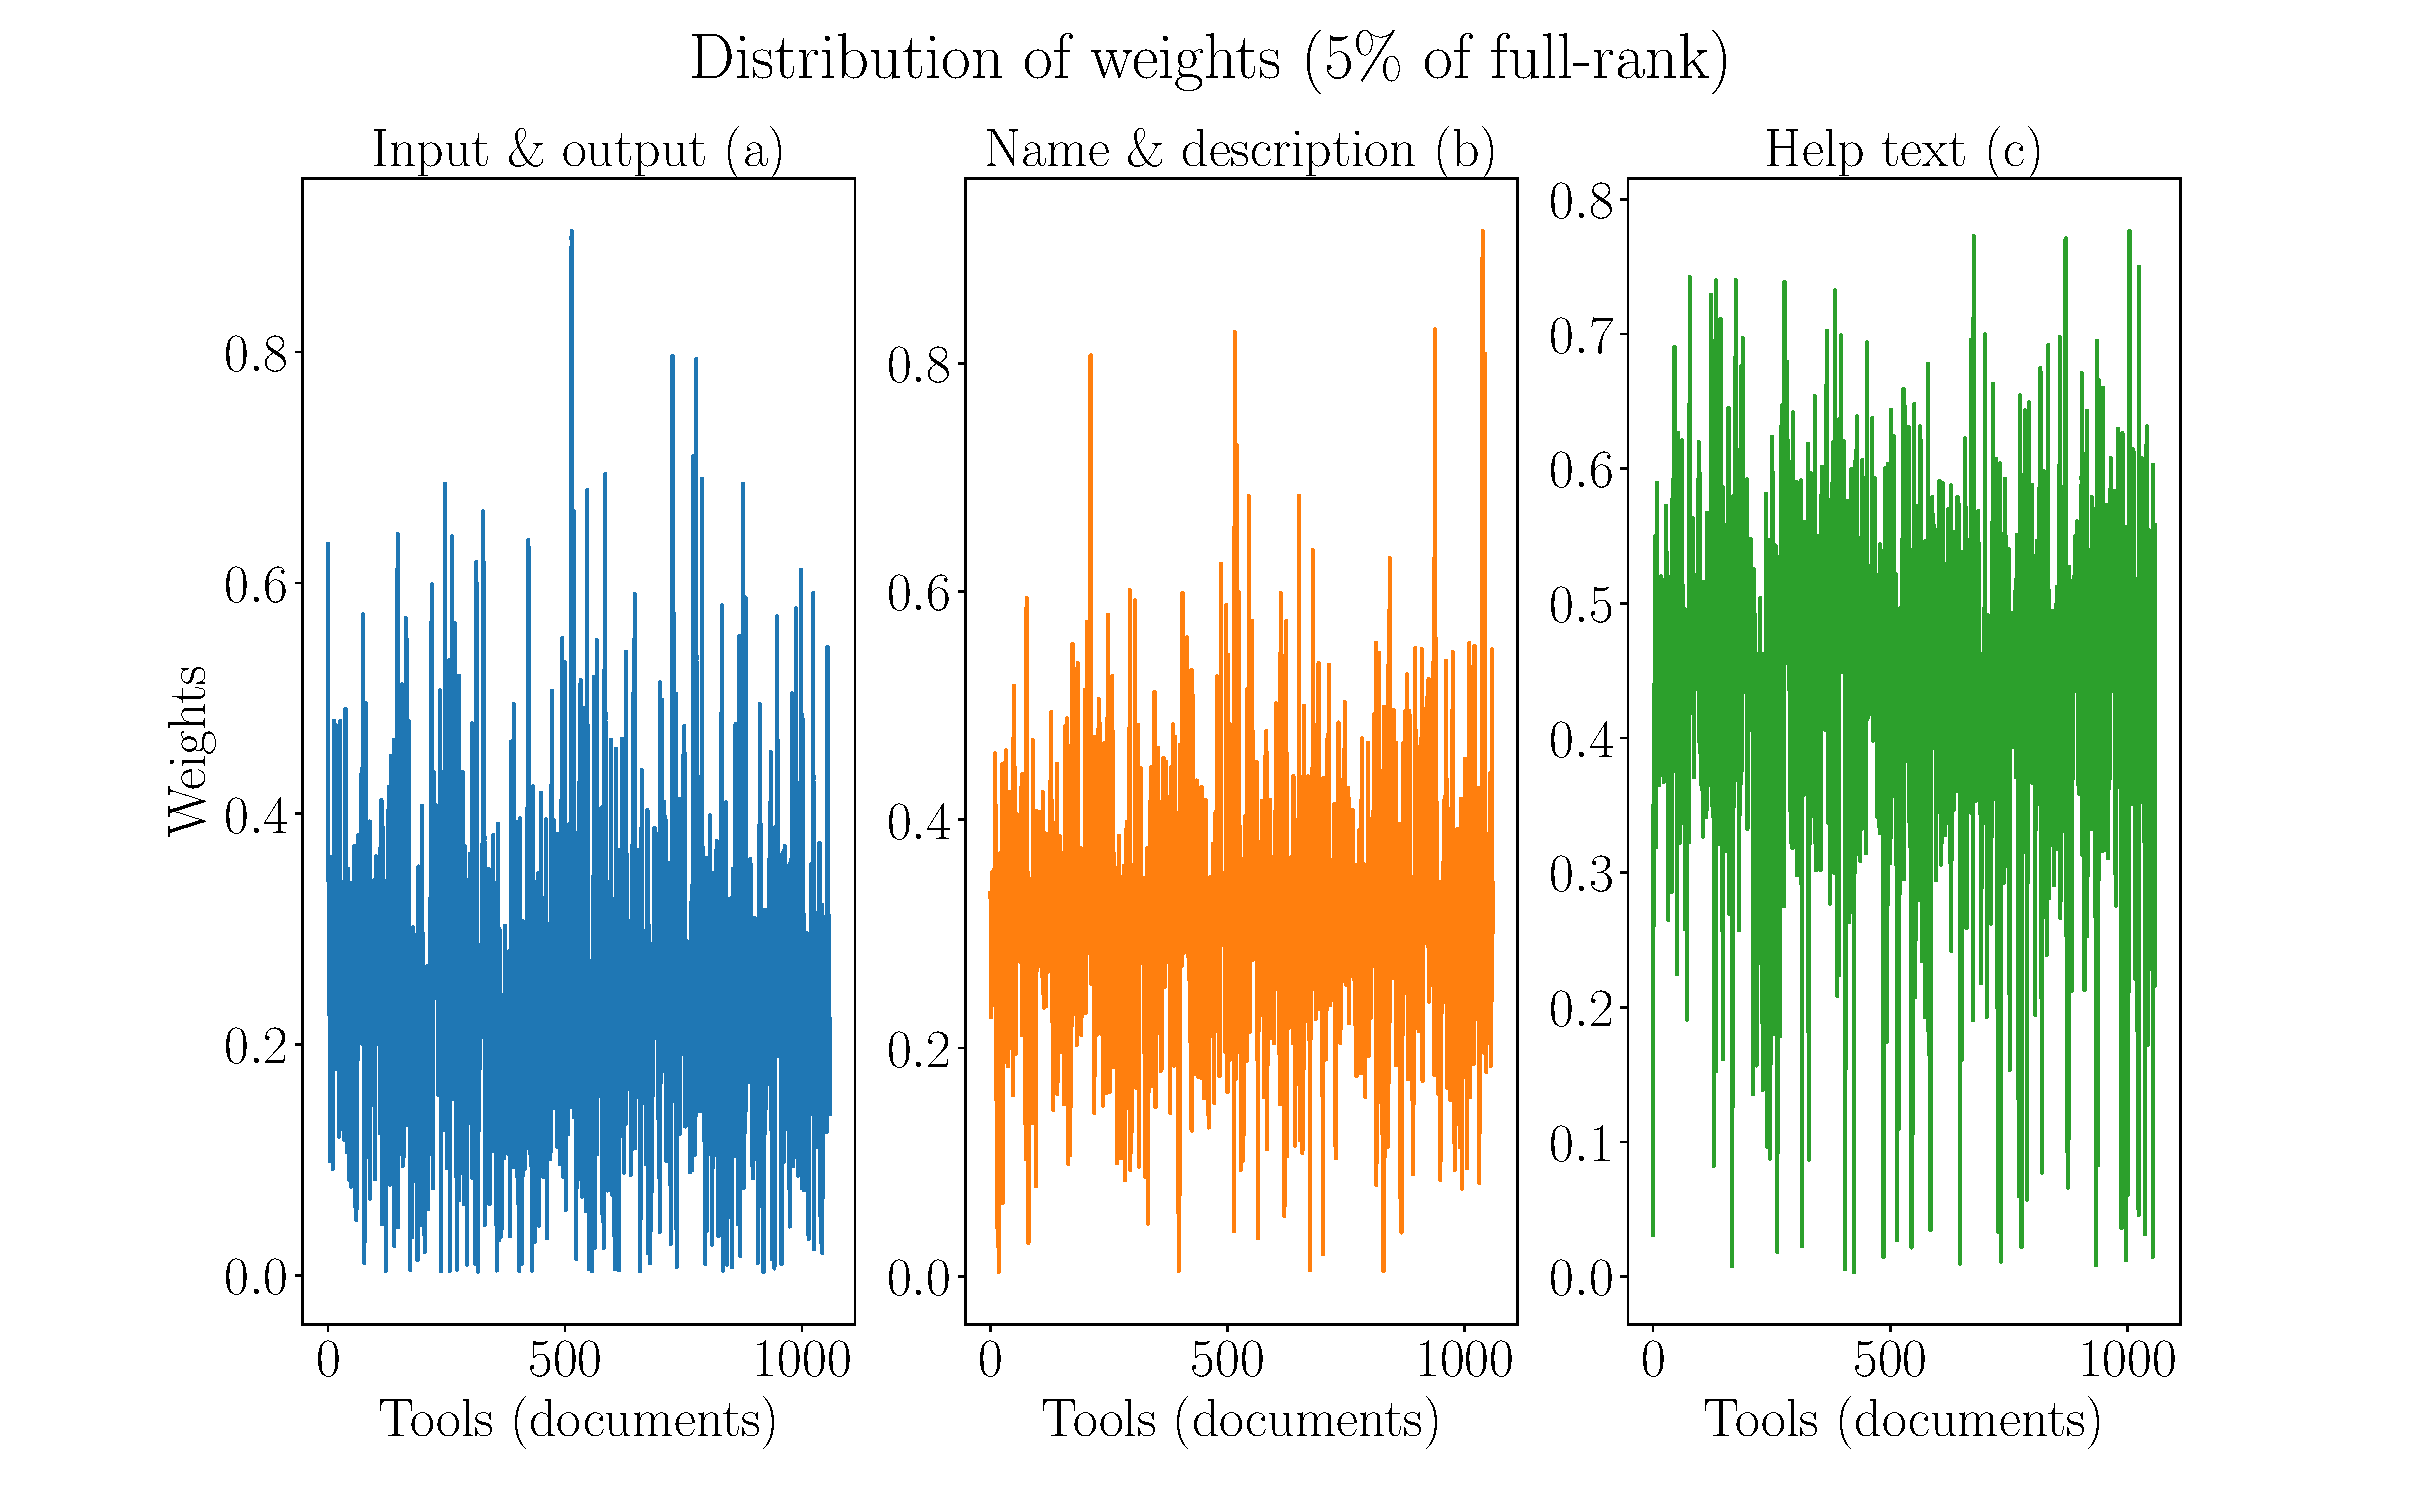
\includegraphics[scale=0.35]{figures/Weights_005.pdf}}
    \caption[Weights distribution 5\% rank]{\textbf{Weights distribution using 5\% of full-rank}: The plot shows the distribution of weights learned by gradient descent optimizer on the similarity matrices for the input and output, name and description and help text attributes. The corresponding documents-tokens matrices contain 5\% of their full-ranks.}
\end{centering}
\end{figure}

\subsection{Improvement verification}
To verify that the matrix rank reduction actually works and learns better similarity scores for tools (documents) which are similar in actual case, we showcase two ways.

\subsubsection{Reduction in error}
We observe drop in mean squared error when we decrease the ranks of the matrices. When we reduce the ranks, the similarity scores for the name and description and help text increase. This increase accounts for their larger weights learned by the optimizer. The weights on an average become more balanced and together with higher similarity scores account for the decrease in the mean squared error. In the absence of true similarity values, this viewpoint might not be completely correct way to establish that we actually improve the performance. To be more certain, we created a visualizer using javascript and html to look through the similar tools and their respective scores and weights for all tools. The next section explains it.

\subsubsection{Visualizer for latent semantic analysis approach}
% screenshots
We see the similar tools for a few selected tools for the different stage of rank reduction and verify if we actually fetch the similar tools.

\begin{figure}[h]
\begin{centering}
    {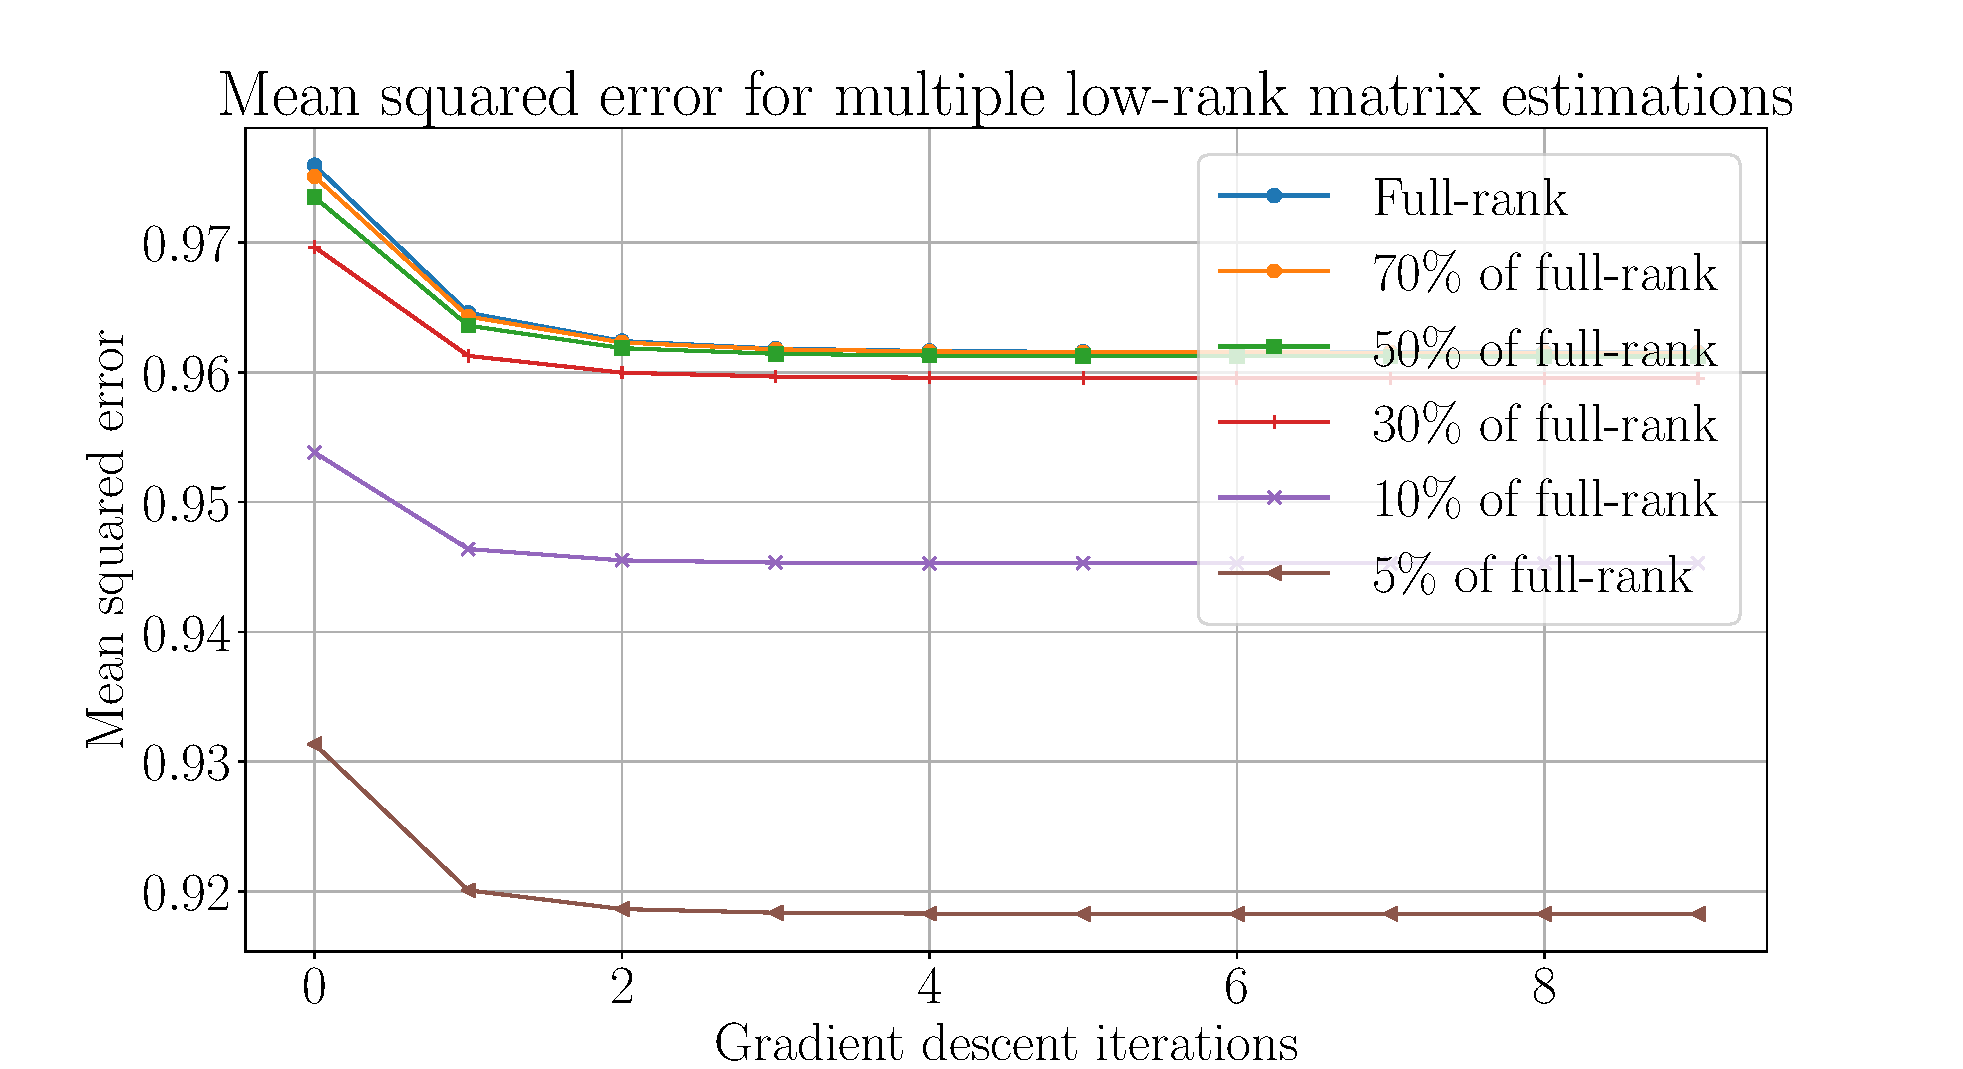
\includegraphics[scale=0.35]{figures/MSE_iterations_low_rank.pdf}}
    \caption[Mean squared error using LSI]{\textbf{Mean squared error using full-rank and multiple estimations of low-rank documents-tokens matrices}: This shows an mean squared error comparison computed using full-rank and various estimations of low-rank documents-tokens matrices. Each line plot shows an average error over all the tools and attributes which drops as we move along the iterations of gradient descent.}
\end{centering}
\end{figure}

\section{Paragraph vectors}

\begin{figure}[h]
\begin{centering}
    {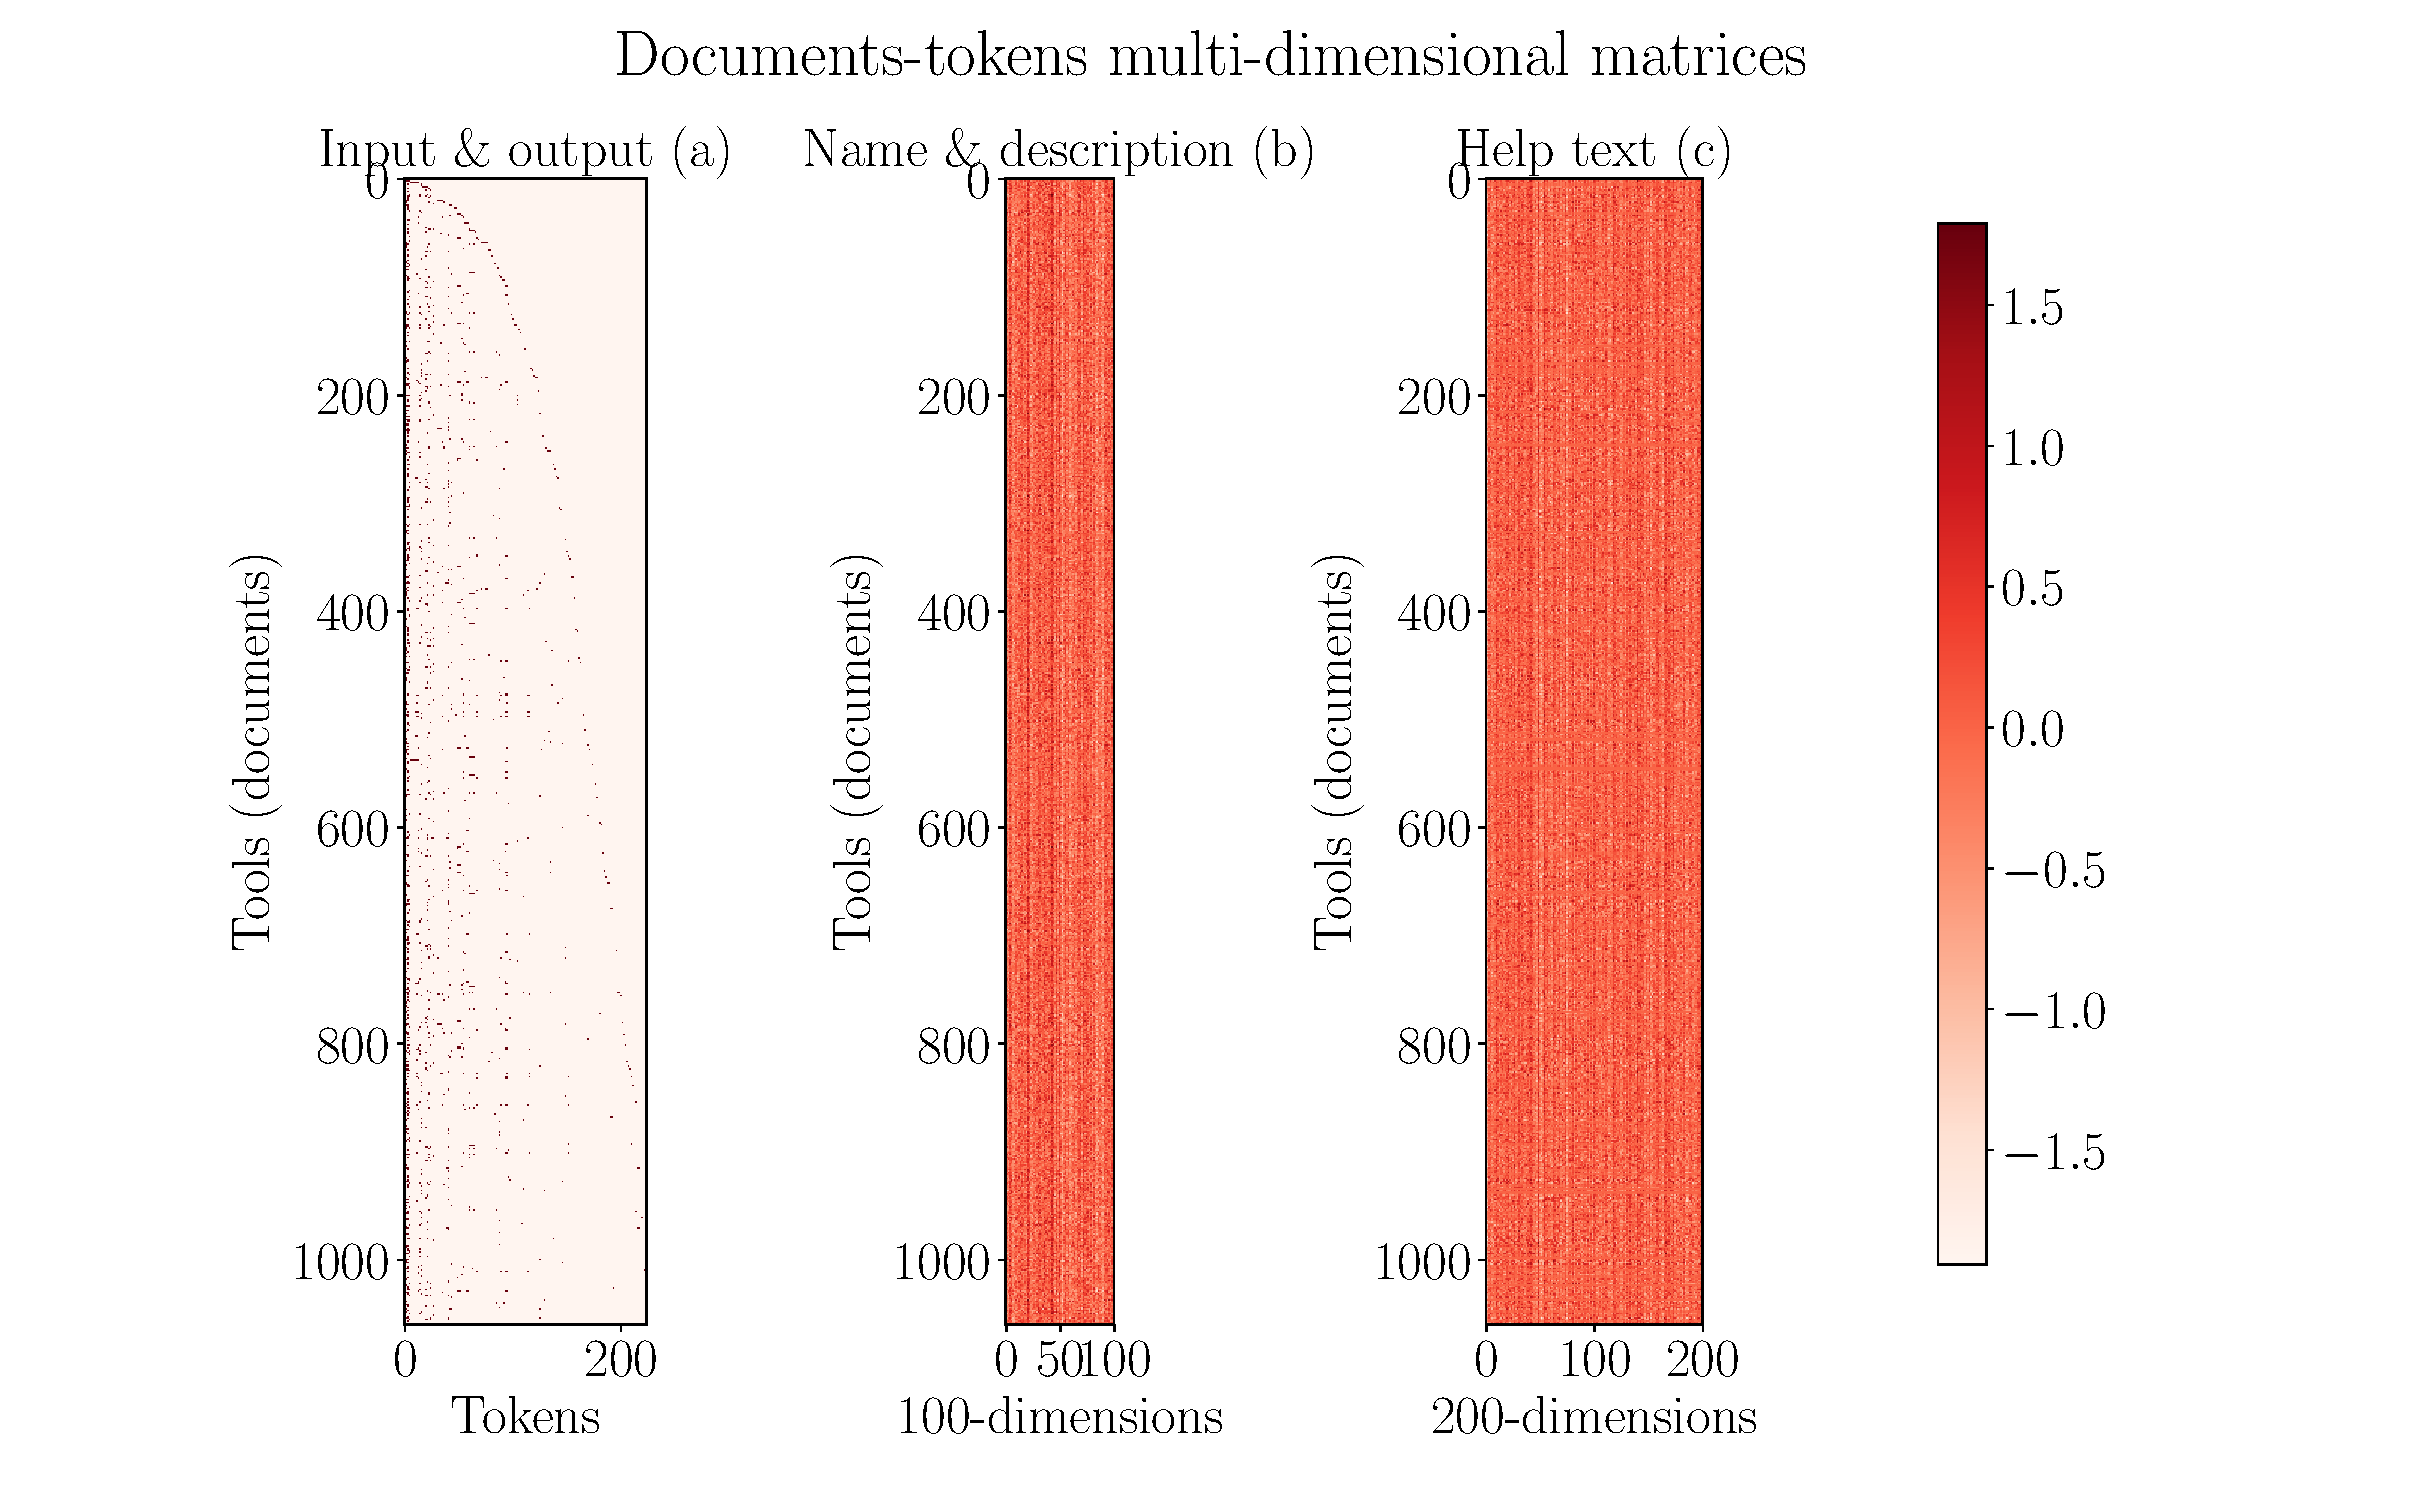
\includegraphics[scale=0.35]{figures/Documents-tokens_doc2vec.pdf}}
    \caption[Documents-tokens matrices for paragraph vectors]{\textbf{Documents-tokens matrices for paragraph vectors approach}: The heatmap shows documents-tokens matrices for input and output file types (a), name and description (b) and help text (c) attributes. The matrix in (a) is a document-token matrix where each entry shows a relative frequency of the token's occurrence. The matrices in (b) and (c) are 100 and 200 dimensional (each row is a document vector) respectively which means that each row of a matrix belongs to a document (paragraph) and is fixed-length and dense in nature. }
\end{centering}
\end{figure}

\begin{figure}[h]
\begin{centering}    
    {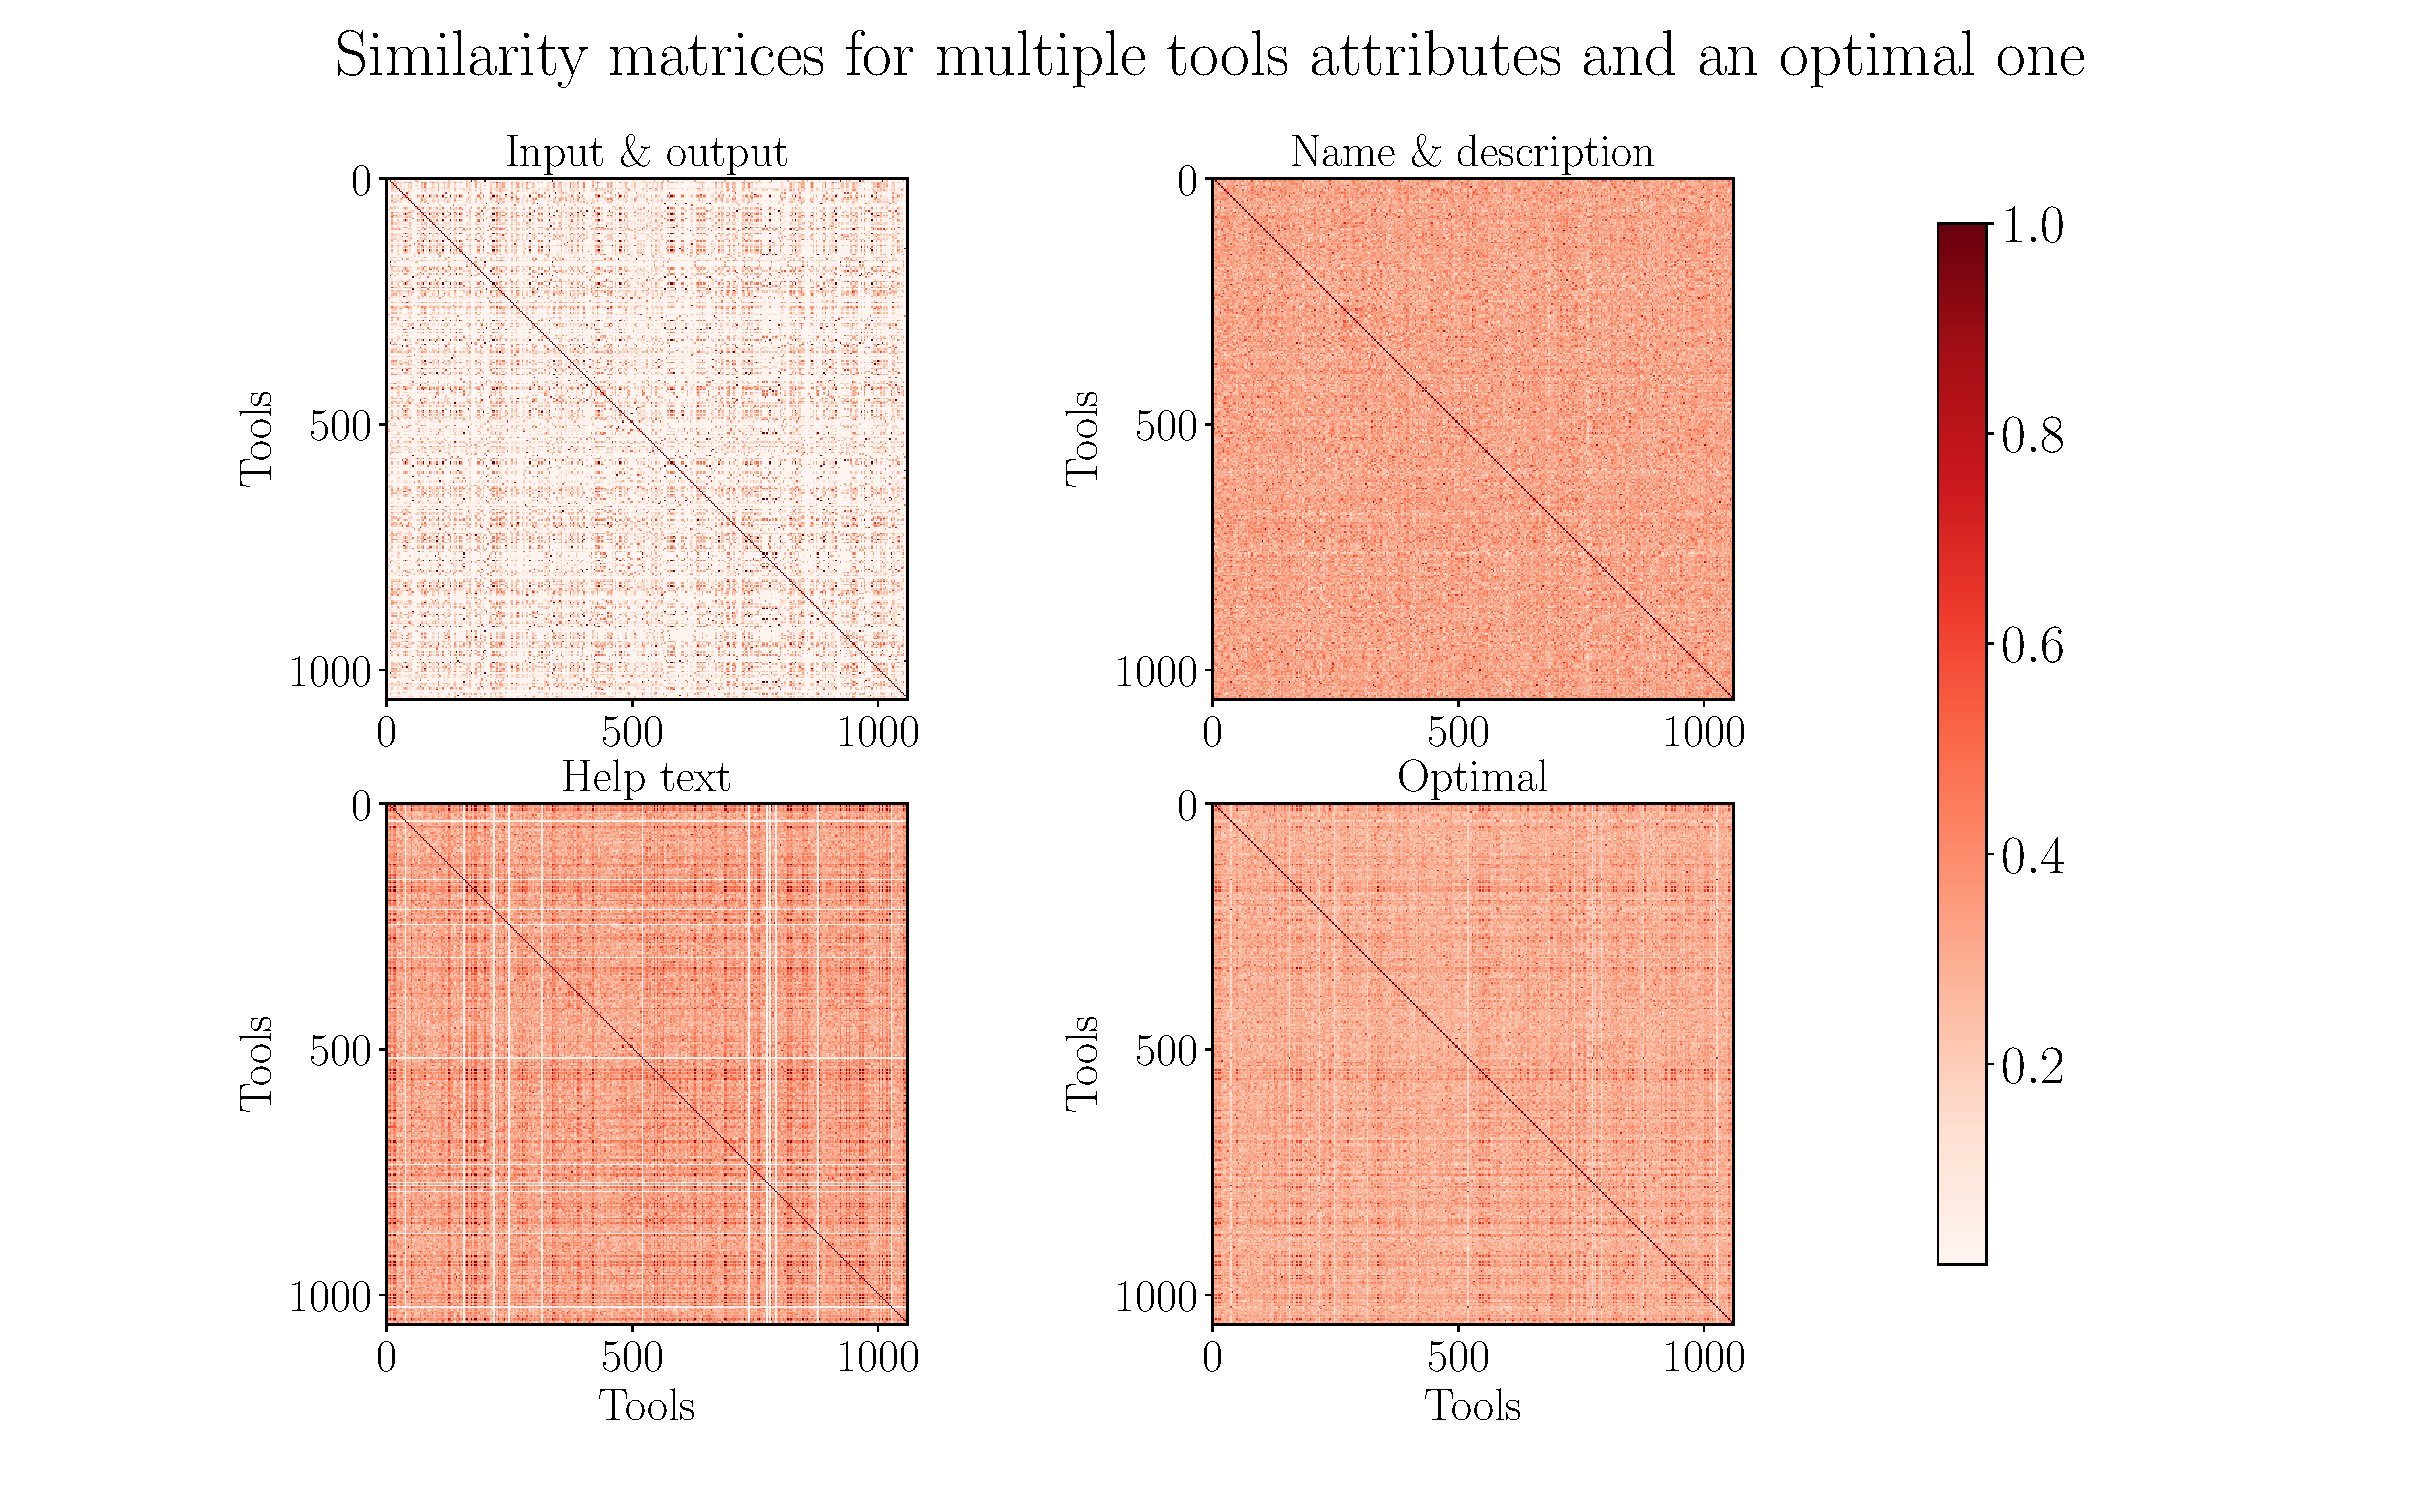
\includegraphics[scale=0.35]{figures/Similarity_matrices_doc2vec.pdf}}
    \caption[Similarity matrices using paragraph vectors approach]{\textbf{Similarity matrices using paragraph vectors approach}: The heatmap shows documents-documents (tools-tools) correlation matrices for input and output (a), name and description (b) and help text (c) attributes. The (d) shows a documents-documents (tools-tools) correlation matrix which is the weighted average computed using (a), (b) and (c) and weights (figure 22) given by the gradient descent optimizer (equation 15). The corresponding documents-tokens matrices are computed as shown in figure 26.}
\end{centering}
\end{figure}

\begin{figure}[h]
\begin{centering}
    {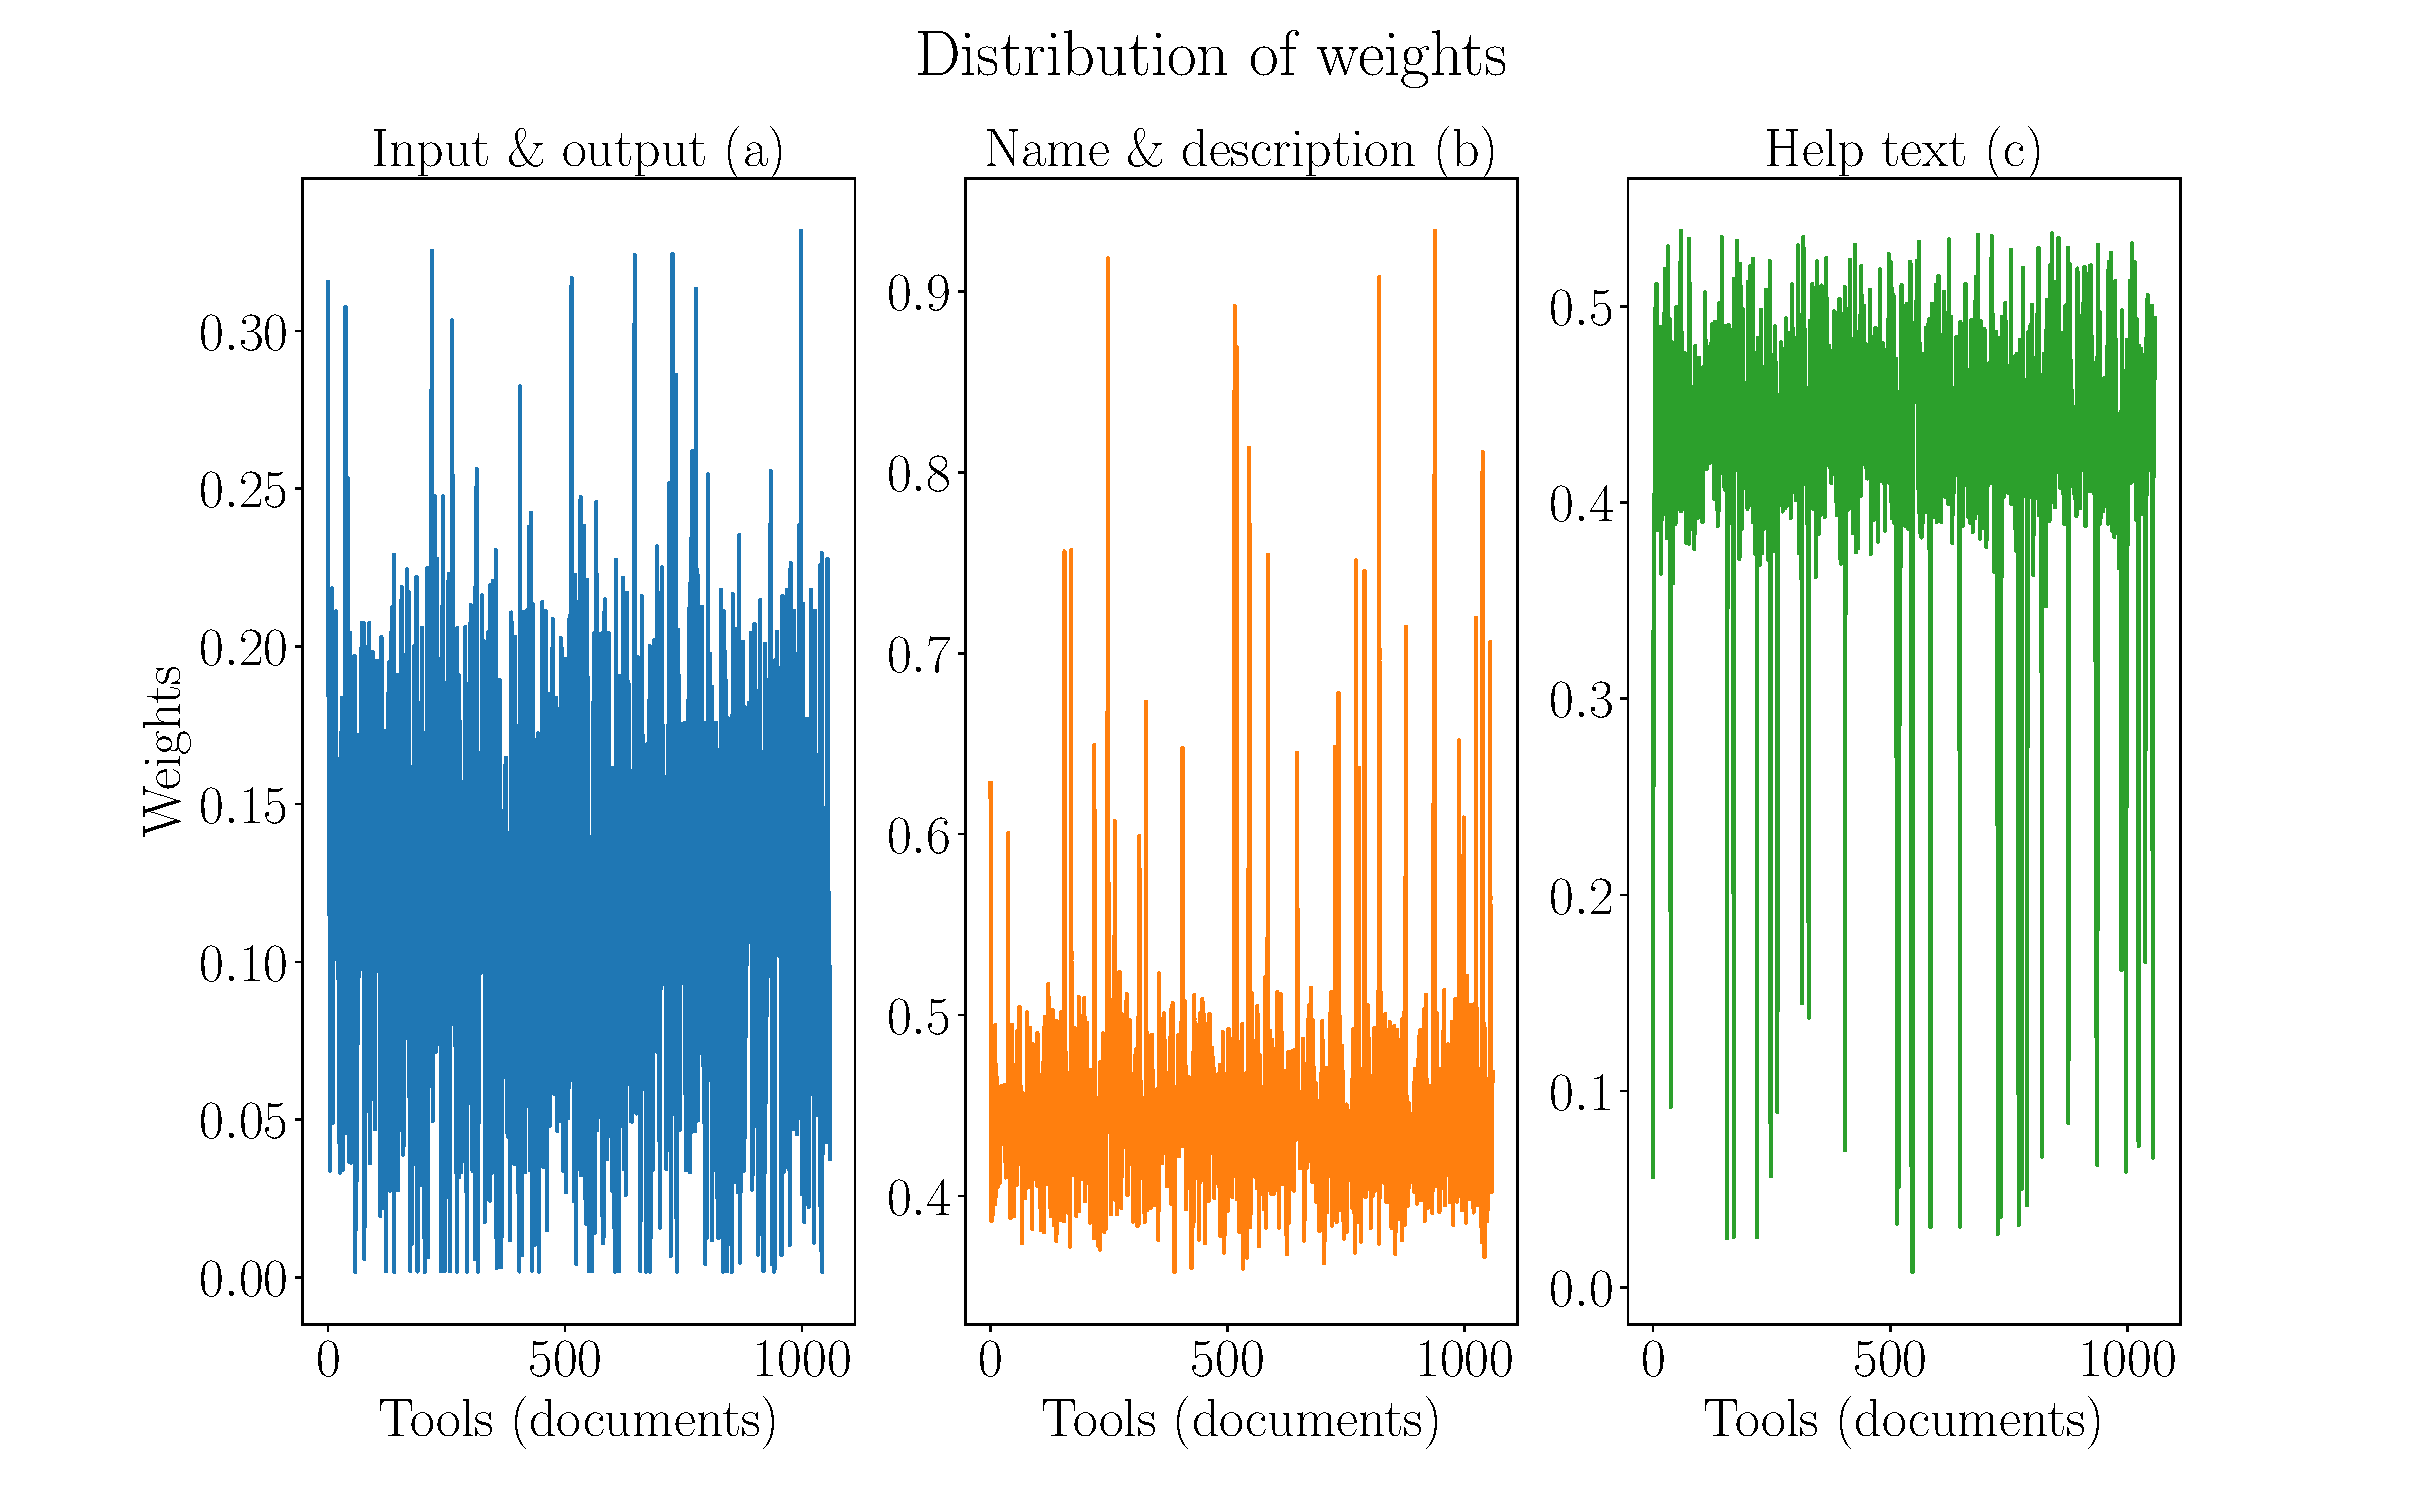
\includegraphics[scale=0.35]{figures/Weights_doc2vec.pdf}}
    \caption[Weights distribution for doc2vec]{\textbf{Weight distribution learnt using paragraph vectors approach}: The plot shows the distribution of weights learned by gradient descent optimizer on the similarity matrices for the input and output (a), name and description (b) and help text (c) attributes. The corresponding documents-tokens matrices are computed as shown in figure 26. }
\end{centering}
\end{figure}

\subsection{Optimization}
\begin{figure}[h]
\begin{centering}
    {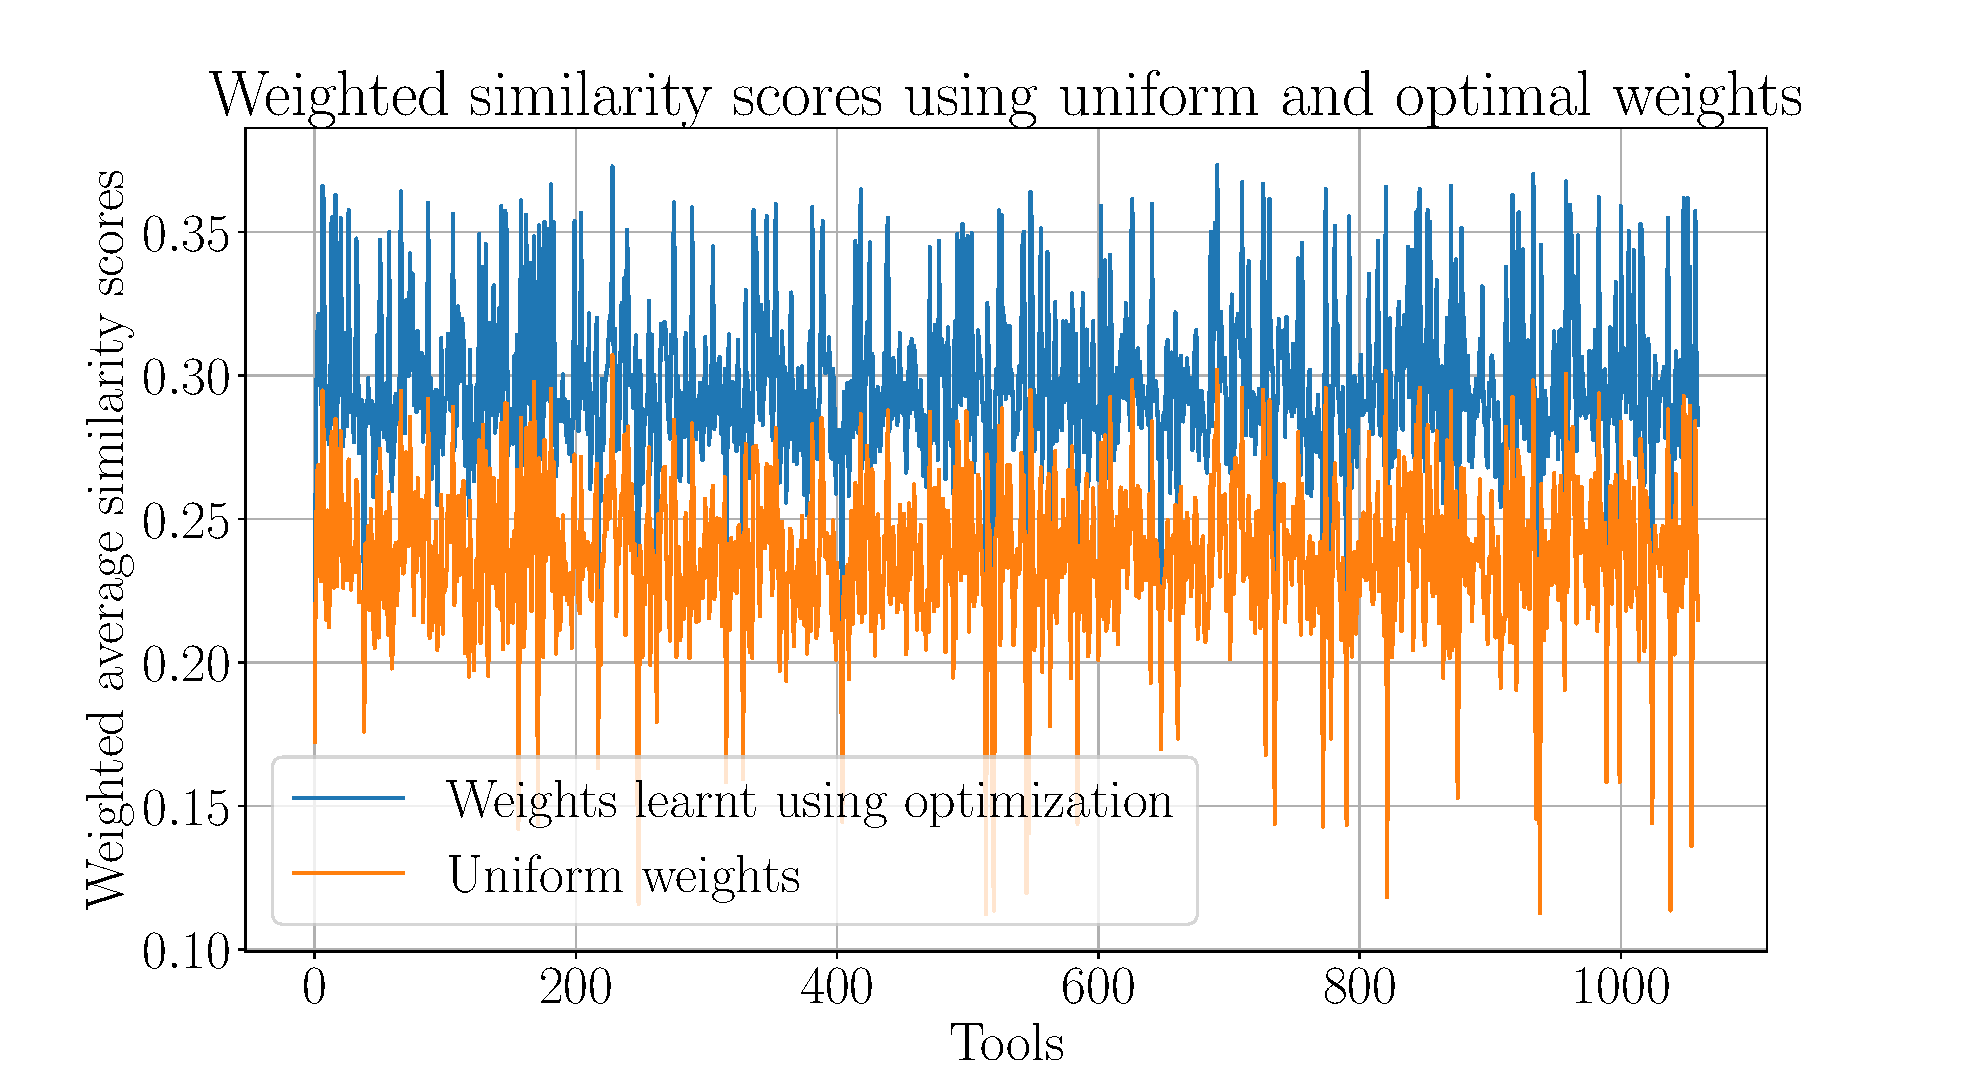
\includegraphics[scale=0.45]{figures/weighted_optimal_uniform_scores.pdf}}
    \caption[Optimal uniform similarity scores]{\textbf{Similarity scores learned using optimal and uniform weights for paragraph vectors approach}: The plot shows a comparison of average similarity scores computed across all tools using weights learned using optimization and uniform weights. }
\end{centering}
\end{figure}


\subsection{Visualizer for paragraph vectors approach}
% screenshots



    \chapter{Conclusion}

\section{Data}
Noisy, no true value, some good, some bad results.




    \chapter{Future Work}

    % bibliography is not in the table of contents per default, add it manually
    % enable the \renewcommand for german header
    % \renewcommand{\bibname}{Literaturverzeichnis}
    \addcontentsline{toc}{chapter}{Bibliography}
    
    \bibliographystyle{ieeetr}
    \bibliography{bib/topic1}
    \newpage
    \thispagestyle{empty}
    \mbox{}
    

\end{document}
